\documentclass[12pt,oneside]{book}
\pagestyle{headings}

% Note that the line below could be modified to suit a
% particular system since the "geometry" package behaves
% differently in Unix, Windows and Mac, especially for the
% top margins.
% Adjust the parameter "top" (measuring the height of the
% space allocated to a header) and "headsep" (measuring
% the distance from the bottom of the header to the
% first line of text.
\usepackage[top=1.3in,left=1.5in,bottom=1in,right=1in,headsep=0.5in]{geometry}

\usepackage{setspace}
\onehalfspacing
%\doublespacing

% Headers and footers for thesis
\usepackage{fancyhdr}

\markboth{}{}
\newcommand\startchapter[1]{\chapter{#1}\thispagestyle{myheadings}}
\newcommand\startappendix[1]{\chapter{#1}\thispagestyle{myheadings}}
\newcommand\startfirstchapter[1]{\chapter{#1}}

% Manual addition of section to Table of Contents
\newcommand\TOCadd[1]{\newpage\phantomsection\addcontentsline{toc}{chapter}{#1}}

% Float Customization
\renewcommand{\floatpagefraction}{0.01}

% Customization of Tables of Contents and List of Figures/Tables
\usepackage{tocloft}
\renewcommand\cfttabpresnum{Table\ }
\renewcommand\cfttabnumwidth{0.75in}
\renewcommand\cftfigpresnum{Figure\ }
\renewcommand\cftfignumwidth{0.80in}
\newcommand{\HRule}{\rule{\linewidth}{0.5mm}}

% Long Table and decimal aligned columns
\usepackage{dcolumn}
\usepackage{longtable}

% Mathematics support
\usepackage{amsmath}
\usepackage{amsthm}
\usepackage{amssymb}


% Text Control
\usepackage{xspace}
\usepackage{textcase}

% Graphics
\usepackage{wasysym}
\usepackage{graphics}
\usepackage{graphicx}   % A package to allow insertion of
                        % external image files



\begin{document}

% Front Matter
\input frontmatter/fm

\newpage

% demonstrated chapters with suggestions and tips
\startfirstchapter{Introduction}
\label{chapter:introduction}




\input chapters/1/sec_intro
\input chapters/1/sec_review
%\pagebreak
\section{My Claims}
Something must be new in this work, no matter how small, since you are getting a graduate degree for it! Tell me about it clearly and succintly right now, just as you did in the abstract. Make an impact here. How about something like the following box:

I make \textit{four} claims which
my dissertation validates:
\\

\framebox{%
\parbox{5in}{
	My new algorithm to solve the problem of doing nothing include these important new features whose practical applicability can be proved both formally and empirically:
	\begin{enumerate}
	\item first feature;
	\item second feature;
	\item everything is much easier to understand, and therefore, easier to implement correctly.
	\end{enumerate}
}}
\\

\noindent Claim 1 and claim 2 are \textit{quantitative} - they will be proven by experiment.

\noindent Claim 3 is \textit{qualitative} - they will be demonstrated by argument.

\subsection{The Importance of My Claims}

Some very important positive consequences
arise from the validation of the above claims.
It is these consequences that comprise a significant
positive contribution to research in the field
of whatever the field is.
\\

\noindent Claim 1 implies that:
\begin{enumerate}
\item{Something profound which applies to:
	\begin{itemize}
	\item {something excellent;}
	\item {something important.}
	\end{itemize}}
\item{Something else just as profound.}
\end{enumerate}

\noindent Claim 2 implies that:
\begin{itemize}
\item{Repeat as above if necessary and useful.}
\end{itemize}

\noindent The consequence of claim 3 is that:
\begin{itemize}
\item{There must be something good coming out of all this work!}
\end{itemize}

\section{Agenda}

This section provides a map of the dissertation
to show the reader where and how it validates
the claims previously made. Here is where I am also presenting my own style of organization which may be totally different from what your supervisor thinks. However, trust me, this is a good solid beginning for a structure. Your supervisor may ask you to change it, but will still appreciate what you have! For each of the chapters below I also give a short summary of what the main focus should be and then I expand on it  a bit within the chapter itself.

\begin{description}
\item[\textbf{Chapter 1}] contains a statement of
the claims which will be proved by this dissertation followed by an overview of the structure of the document itself.
\item[\textbf{Chapter 2}] describes in details the open problem which is to be tackled together with its context, its impact and the overall motivation for the research overall.
\item[\textbf{Chapter 3}] gives the new research, its methodology, the algorithms involved, the new solution, the new work done. Formal proofs and arguments are made here. This is the first of the two contributions expected in a thesis for a graduate degree.
\item[\textbf{Chapter 4}] is where the experiments and the methodology for them is fully described. The first part includes all details of how the empirical side of the research has been conducted. Note that not every thesis has this empirical portion.
\item[\textbf{Chapter 5}] includes the evaluation of the data presented above and the comparisons with the work of others, to show how much better the new approach is. This is the second of the two contributions expected in a thesis for a graduate degree. Note that this part could be consolidated into the chapter above.
\item[\textbf{Chapter 6}] contains a restatement of the claims and results of the dissertation. It also enumerates avenues of future work for further development of the concept and its applications.
\end{description}

The list above is not complete. Chapter 3 actually includes a lot more, as I could not resist placing in it a few \LaTeX examples to help you along. This document is not a primer for \LaTeX, but there is no harm done in giving a little help.

\startchapter{The Problem to be Solved}
\label{chapter:problem}

\newlength{\savedunitlength}
\setlength{\unitlength}{2em}

Here is where you tell me what is the problem you have been working on for the past few months (or years). I want all the details and you should not be timid about being too tutorial, except that you do not want to cross the line towards writing a textbook. However consider carefully that \textit{communication} implies conveying ideas to other people, while \textit{effective communication} occurs when your message is clearly understood. Remember that your audience must understand your message before they can agree with you.

Ask yourself:
\textit{who is your audience?} You might think of your supervisor who knows everything and you want to impress with your knowledge. I think instead of the graduate students who will be reading this thesis which is, after all, a property of the university. It is published as a university technical report so that others may learn by reading it. Then teach them! Be a bit tutorial. Even the expert external examiner will be impressed by your clarity of exposition if he or she does not need to read paragraphs twice in order to understand - something which people with PhDs and big egos find particularly irritating.

On the other hand, do not go too far and give trivial definitions from concepts learned in a 3rd year undergraduate courses, else you might find yourself in trouble when having to remember the details during an oral examination.

My approach is to put everything necessary to make clarity for
the problem the main goal of this chapter, assuming an intelligent and well prepared reader who already has a Bachelor degree in an appropriate subject.

Once I understand the problem clearly and its nuances (it may not be what I expected after all), I also need to know why the problem is important, what its impact is and what its application, if any. Here you are free to elaborate and write as much as you think is necessary to avoid the examination doubt that you have a brilliant new solution to a trivial and unimportant issue.

I suggest reading various books on how to do research and set up problems. The best for me was "The Craft of Research" by Wayne Booth \cite{booth1}, which can be found in the main library at Q180.55 M4B66. From there I have transferred to my writing a fairly simple structure for talking about the topic of the research, with the question to be asked and its motivation and significance. It goes as follows:
\begin{enumerate}
\item {\textit{I am trying to learn about (working on, studying...)}}
\item {\textit{because I want to find out....}}
\item {\textit{in order to understand...}}
\end{enumerate}

Another way of looking at this is to ask the
\textit{what}, \textit{why} and \textit{where}, starting from a \textit{setting} of the problem with a first point A, stating what the \textit{goal} is at point B and having an \textit{action link} between the two which will encompass your new solution. As surprising as this may be to some of you, I found reading a book from Microsoft very useful: "Beyond Bullet Points: Using Microsoft Office PowerPoint 2007 to Create Presentations That Inform" \cite {atkin}. The goal of the book is to improve presentations with Power Point, but there is a lot that can be transferred towards \textit{effective communication} for a thesis.

In summary, my view of the second chapter on
\textit{"The Problem to be solved"} is as follows:
\begin{enumerate}
\item {\textit{Not} all the background and definitions (boring!) - use instead just-in-time explanations as needed in every context as it comes up;}
\item {Motivation in depth;}
\item {Tutorial high level explanation, where it is important to choose the right pitch: who is the audience? who are you teaching here?}
\item {Make it exciting, make it current, make it important - why do I want to keep reading?}
\item {Should you list here the solutions from other researchers? I think not, list instead the different facets of the problems that other researchers have attacked.}
\item {A taxonomy can be extremely useful to place your problem and its particular special features within the perfect context of the overall area, as you need to make sure that the reader understands perfectly what you are trying to solve.}
\end{enumerate}


\setlength{\unitlength}{\savedunitlength}

\startchapter{The New Approach and Solution}
\label{chapter:newsol}

This is where you go all out and tell us all about your new discovery and research related to the problem in the previous chapter. No arrogant sweeping statements which cannot be fully justified, but no false modesty either. You must impress your reader that you have accomplished something.

Simply summarized, this chapter should be comprised of at least two main sections, each with appropriate subsections. The first section should describe:
\begin{itemize}
\item {what the new approach is;}
\item {what is really totally new;}
\item {what is incrementally new;}
\item {what you built upon.}
\end{itemize}

The second part should describe fully how the new approach works, both with the overall theoretical exposition (e.g. an algorithm) and with as many examples as necessary for clarity. Remember that if the reader does not understand fully, you will get a lot of questions and doubts. Good examples, good figures, good diagrams with super clear tutorial explanations can be a joy to read and make even a small contribution appear to be more impressive. Are you afraid that if you are too tutorial your work will not seem as deep and difficult? Only shallow people will make such a superficial evaluation, have trust instead in the wisdom of your supervisory committee.

Use at least one good example throughout, and even better if this is one of the examples you used in Chapter 2 to describe the original problem.

By the way, this would be the first chapter I would write. This is what I know best right now, as I just finished working on it. It is clear to me and on the tip of my fingers. Start with your strengths! The second chapter I would write is the next one about the experiments, followed closely by chapter 2 describing the problem. It may not seem intuitive to you, but it works and it is the most productive way I ever found to finish a document.


\input chapters/3/sec_latexhelp

\startchapter{Experiments}
\label{chapter:Exp}

Assuming you have some experimental results to support your claims this is where all the data is reported. There are a few issues you should consider before dumping a lot of stuff here, or it will lose its effectiveness.

First of all you must describe precisely the experimental setup and the benchmarks you used. In any scientific discipline an experimental result is only good if it is reproducible. To be reproducible then somebody else must have sufficient details of the setup to be able to obtain the same data. Thus the first section in this chapter is a super precise history of the decisions made towards experimentation, including mentions of the paths which became infeasible. The setup must be valid and thus your description of it must prove that it is indeed sound. At times, terrifying times, when writing this section, both supervisor and student realize belatedly that something is missing and more work needs to be done!

The second portion of this chapter is dedicated the the actual results. At least two issues arise here:
\begin{enumerate}
\item {Should all the data be reported here or should some be placed in the Appendix?}
\item {Should this be an exposition of the raw facts and data or should it include its analysis and evaluation?}
\end{enumerate}

There are no definite answers here, but I follow a few rules.

\textit{Should all the data be reported here or should some be placed in the Appendix?}
    \begin{itemize}
    \item{If there is a large number of tables of data, it might be better to present here only a handful of the most significant ("best") results, leaving all the rest of the data in the Appendix with proper linkages, as it would make the chapter so much more easily readable (not to mention limiting the struggle with a word processor for the proper placement of tables and text).}
    \item{Use an example throughout, call it a "case study" to make it sound better, so that all the data and results are somehow linked in their logic, and even better if this is one of the examples you used in Chapter 2 to describe the original problem.}
    \item{Highlight in some manner the important new data, for example the column of your execution speed where all the numbers are much smaller. Make the results highly easy to read!}
    \item{It is normally expected that data should be presented only in one form and not duplicated, that is, you are not supposed to include both a table of raw numbers and also its graphical representation from some wonderful Excel wizard. I tend to disagree. I would not wish to see every results repeated in this manner, but some crucial ones need to be seen in different manners, even with the same information content, in order to show their impact. One good trick is to place the more boring tables in the Appendix and use wonderful graphs in this chapter.}
    \item{This is the one chapter where I would splurge and use colour printing where necessary, as it makes an \textit{enourmous} difference.}
    \end{itemize}

\textit{Should this be an exposition of the raw facts and data or should it include its analysis and evaluation?}
     \begin{itemize}
    \item{Is the evaluation of the data really obvious? For example you have 10 tables to show that your chemical process is faster in development and gives purer material - you may simply need to highlight one column in each table and state the obvious.}
    \item{Most results are not that obvious even if they appear so. Moreover this is where you are comparing your \textit{new} results to data from other people. I usually describe other people's work at this point and make comparisons. That is why I prefer to talk about the analysis and evaluation of the results in a separate chapter.}
    \item{There is absolutely no clear structure here which is best.}
    \end{itemize}

\startchapter{Evaluation, Analysis and Comparisons}
\label{chapter:eval}

For a Master's research this chapter represents the critical part where \textbf{you} are truly evaluated to determine whether you should be given your degree. Even more so for a PhD. Consider carefully what the University calendar states regarding the expectations for a master's thesis, paraphrased here.

\begin{enumerate}
\item {\textit{A Master?s thesis is an original lengthy essay.} The main implication here is that the essay is original, that is, it is completely newly written by you and does not contain any writings from others unless precisely quoted. Any paraphrased items must be cited.}
\item {\textit{It must demonstrate that:}
    \begin{itemize}
    \item {students understand research methods;}
    \item {students are capable to employ research methods;}
    \item {students demonstrate command of the subject.}
    \end{itemize}}
\item {\textit{The work may be based on:}
    \begin{itemize}
    \item {original data;}
    \item {original exercise from scholarly literature;}
    \item {data by others.}
    \end{itemize}}
\item {\textit{The work must show that:}
    \begin{itemize}
    \item {appropriate research methods have been used;}
    \item {appropriate methods of critical analysis supplied.}
    \end{itemize}}
\item {\textit{The work must contain:}
    \begin{itemize}
    \item {evidence of some new contribution;}
    \item {evidence of a new perspective on existing knowledge.}
    \end{itemize}}
\end{enumerate}

Only the last point uses the attribute \textit{new} and it refers almost entirely to giving a new perspective and analysis, even if based on data from others. This truly implies that this current chapter on evaluation and analysis of results is the most important and must be written with care. You are demonstrating here that, even if given data and methods from others, your skills of critical judgment and analysis are now at the level that you can give professional evaluations.

Things are slightly different for a PhD. According to the Graduate Calendar: \\ 
\textit{a doctoral dissertation must embody original work and constitute a significant contribution to knowledge in the candidate's field of study. It should contain evidence of broad knowledge of the relevant literature, and should demonstrate a critical understanding of the works of scholars closely related to the subject of the dissertation. Material embodied in the dissertation should, in the opinion of scholars in the field, merit publication.}

\textit{The general form and style of dissertations may differ from department to department, but all dissertations shall be presented in a form which constitutes an integrated submission. The dissertation may include materials already published by the candidate, whether alone or in conjunction with others. Previously published materials must be integrated into the dissertation while at the same time distinguishing the student's own work from the work of other researchers. At the final oral examination, the doctoral candidate is responsible for the entire content of the dissertation. This includes those portions of co-authored papers which comprise part of the dissertation.}

The second paragraph makes it clear that one must emphasize what is new and different from others, without arrogance, yet without being too subtle either. The first paragraph implies that for a PhD it is required that one approached an important open problem and gave a new solution altogether, making chapters 3, 4, 5 all part of the body of research being evaluated. In fact at times even the problem may be entirely new, thus including chapter 2 in the examination. This is in contrast to a Master's degree where the minimum requirement is for chapter 5 to be original.




\startchapter{Conclusions}
\label{concl}

My first rule for this chapter is to avoid finishing it with a section talking about future work. It may seem logical, yet it also appears to give a list of all items which remain undone! It is not the best way psychologically.

This chapter should contain a mirror of the introduction, where a summary of the \textit{extraordinary} new results and their wonderful attributes should be stated first, followed by an executive summary of how this new solution was arrived at. Consider the practical fact that this chapter will be read quickly at the beginning of a review (thus it needs to provide a strong impact) and then again in depth at the very end, perhaps a few days after the details of the previous 3 chapters have been somehow forgotten. Reinforcement of the positive is the key strategy here, without of course blowing hot air.

One other consideration is that some people like to join the chapter containing the analysis with the only with conclusions. This can indeed work very well in certain topics.

Finally, the conclusions do not appear only in this chapter. This sample mini thesis lacks a feature which I regard as absolutely necessary, namely a short paragraph at the end of each chapter giving a brief summary of what was presented together with a one sentence preview as to what might expect the connection to be with the next chapter(s). You are writing a story, the \textit{story of your wonderful research work}. A story needs a line connecting all its parts and you are responsible for these linkages.


% real chapters
\startchapter{A one-dimensional model of scaling in Reverse Osmosis: ROSSpy}
\label{ROSSpy_chapter}

\section{Introduction}
Desalination technologies, most notably reverse osmosis (RO) \cite{Malaeb2011ReverseReview}, are imperative for meeting the 6th UN Sustainable Development Goal \cite{Jones2018TheOutlook} of universalizing potable freshwater. Arid Middle-Eastern countries, who are both relatively affluent and geographically prone to water scarcity, are embracing RO desalination to satisfy domestic water needs; Israel, for example, supplies $\frac{3}{4}$ of its domestic water from desalination \cite{Shemer2017SustainableImpact} and Saudi Arabia is responsible for $\approx 22\%$ of global water desalination \cite{Council2021WaterPrivatization}. RO is the most economical desalination technology \cite{Karime2008ROPlant,Hafez2003EconomicsStudy}, however, it remains insufficiently efficient and economical for the low-resource communities. RO efficiency can be improved \cite{Elimelech2011TheEnvironment,Semiat2008EnergyProcesses} a) with energy recovery devices \cite{Amy2017Membrane-basedProspects}, that allow RO to approach the thermodynamic limit of desalinating seawater \cite{Zarzo2018DesalinationFuture}, and b) by mitigating membrane fouling such as scaling \cite{Warsinger2015ScalingReview,Khan2013SourceSea,Tang2014FoulingPlant,Shmulevsky2017AnalysisMembranes}, where minerals deposit upon the membrane surface and decrease membrane permeability such that greater applied pressures and energy usage are required to maintain a permeate flux over time. Scaling occurs mechanistically either through homogeneous precipitation from the highly concentrated brine byproduct of RO \cite{VanWagner2009EffectPerformance,Belfer1998SurfaceMembranes} -- which is itself hazardous \cite{Fernandez-torquemada2012DispersionPlants,Clemens1955ToxicityWells,Allen1989ApparatusBrine,Munn1989EffectCrops} but can be processed into useful salts \cite{Allen1954ProcessBrine,Fenton1992DesalinationWells} in zero-liquid waste management systems \cite{Jeppesen2009MetalConcentrate,Mavukkandy2019BrineGeneration} or used in mixing-entropy batteries \cite{Ye2019Charge-FreeMaterials} -- or through heterogeneous deposition upon nucleation sites on the membrane surface \cite{Karabelas2014IncipientChannels,Warsinger2018InorganicOsmosis}. The heterogeneous mechanism specifically occurs in a hyper-concentrated layer adjacent to the membrane called the concentration polarization (CP)   \cite{McCutcheon2006InfluenceOsmosis,Murthy1997EstimationModel,Gruber2011ComputationalSystems,Sablani2001ConcentrationReview,Zydney1997StagnantSystems,Li2016Three-dimensionalChannel}, which is achieved as a consequence of the no-slip boundary condition -- analogous to the capillary effect -- that prevents the CP from mixing with the bulk solution since the velocity gradient of the fluid reaches zero adjacent to the stationary filtration membrane \cite{Rapp2017Fluids}. 

Scaling, unfortunately, is experimentally elusive \cite{Hu2014Real-timeSpectroscopy,Butt1995IdentificationAutopsy,Sheikholeslami2003KineticsM}. Computational programs \cite{Giere2009IsExperimentation,Wijmans1995TheReview} may supplement experimental procedures \cite{Lenhard2007ComputerModeling,Chai2007UltrasoundModules} as a means to investigate scaling and optimize RO efficiency; however, current programs are either unspecific to RO \cite{2018ZeroPHREEQC} or focus upon other aspects of RO: e.g. plant operation \cite{DesalitechROSASoftware,Chee2018PerformanceSoftware,SysCAD2020PHREEQCUnit,Bouchareb2019ExperimentalDesalination}, permeate flux \cite{Xu2012TOUGHREACT.0,Steefel2015ReactiveSimulation}, brine geochemistry \cite{Kundu2018TechnicalTechnology}, or fluid dynamics of the CP \cite{Walker2003AssessmentReaction}. Mathematical programs \cite{Radu2014ASystems,Karabelas2019PredictionSimulator} and some with a user interface \cite{SoftwareReverseOsmosis,Strubbe2018CalibrationFull-Scale} have been developed that simulate RO scaling, however, these lack an application programming interfaces (APIs), which is essential for the broad analyses, over a continuum of variables, that could accelerate geochemical scaling research. 

We therefore developed a unique one-dimensional model that captures both the geochemistry of scaling equilibria and the reactive transport of desalination, in contrast to existing one-dimensional RO models that utilize the steady-state approximation and the solution-diffusion model \cite{Strubbe2018CalibrationFull-Scale}. This one-dimensional RO model -- similar only to the WaterTap model \cite{NAWI2021WaterTap} -- is critically amenable with PHREEQC \cite{Parkhurst2015PhreeqcRM:PHREEQC,Charlton2011ModulesLanguages}, which provides a rigorous and open-source numerical implementation of our model, similar to previous studies of scaling \cite{Mitrouli2016CalciumExperiments,Warsinger2018InorganicOsmosis} and RO \cite{Bein1993OriginBrine,Wilson1993GeochemistryFormations,Casas2012SeawaterElectrodialysis,Yan2017ReverseVelocity}. We exemplify our model through replicating experimental literature and conducting numerous sensitivity analyses across continuums of parameter values. We further developed the only, to our knowledge, open-source API of RO reactive transport (ROSSpy: RO Scaling Software in Python) based upon our model, which fulfills identified needs of a scaling software for RO research \cite{Karabelas2020ScalingTools}, where users can create, execute, process, visualize, and export simulations with predicted scale mass per membrane filtration area ($\frac{g~scale}{filtration~m^2}$) and ionic brine concentrations. Developers are encouraged to contribute to ROSSpy, which we believe is an important stride towards satisfying research needs in scaling and ultimately reducing water insecurity, especially in low-resource contexts. 

\section{Methods}

\subsection{Conceptual}

Our model represents RO desalination as a one-dimensional reactive transport process along the membrane-solution interface. The feed is represented by the single-domain model in Figure S4, where the bulk and CP solutions are aggregated into a single solution, as opposed to the more resolved dual-domain model, where the bulk and CP solutions are distinguished (Figure S5) \cite{Chen2016AssessingModel,Scruggs2019TheInterface,Greskowiak2015AUVI,Mieles2012AnalyticalSystem}. The dual-domain remains elusive within the confines of PHREEQC code (Section 6 of the Supporting Information) and moreover we demonstrate that the single-domain model is sufficient to recapitulate experimental results. Our model represents feed at the RO inlet with the Dirichlet boundary condition \cite{Moes2006ImposingMethod,Bazilevs2007WeakMechanics} -- a mathematical description of constant conditions at a model boundary -- where the influent feed is assumed to be an infinite reservoir and thus its concentration is immutable. Our model represents the RO outlet with the Cauchy boundary condition \cite{Gosses2018ExplicitModels} -- a mathematical description of dynamic conditions at a model boundary -- where the effluent concentrations dynamically depend upon desalination. A glossary of parameters and variables for the equations and calculations are provided in Table S1.


\subsection{Numerical}
The geochemistry and reactive transport components of our RO model are numerically detailed in the following sub-sections. 

\subsubsection{Permeate Flux}
The permeate flux in our model is assumed to be 100\% water, similar to other RO models \cite{Li2012OptimalDesalination}, and it is calculated as the change in moles ($\Delta \Phi_{e}$) of feed solution in any examined cell $e$. Permeate flux is proportional to the difference between feed pressure $P$ and osmotic pressure $\pi$ \cite{VanWagner2009EffectPerformance,Schock1987MassModules,Lonsdale1965TransportMembranes}
\begin{equation} \label{pressure_differential}
    \Delta \Phi_{e} ~ \alpha ~ (P - \pi),
\end{equation} 
however, these pressures are not readily measured or reported; hence, we calculate the permeate flux via two comparable methods that are elaborated in the following sub-sections.

\paragraph{Method 1: Linear permeate flux}
One method assumes that permeate flux decreases linearly along the RO module. This causes the concentration -- which is represented by the concentration factor (CF) \cite{McCaffrey1987TheHalite.,Casas2012SeawaterElectrodialysis,Kartashevsky2015PhosphateEffluents,Yan2017ReverseVelocity,Evangelista1985APlants}
\begin{equation} \label{cf_definition}
    CF = \frac{initial}{final}~,
\end{equation}
as the quotient of initial to final ionic concentrations (influent vs. effluent), solution masses, or permeate moles \cite{Casas2012SeawaterElectrodialysis,Yan2017ReverseVelocity} -- to increase exponentially along the RO module. The negative slope of permeate flux is calculated between the first cell $1$ and the last cell $n$
\begin{equation} \label{flux_slope}
    slope = \frac{(\Delta \Phi_{n}-\Delta \Phi_{1})}{n}~,
\end{equation}
where the simulated membrane-solution interface is discretized into $n$ equal fractions (cells) of the total module length $l_{module}$. The permeate fluxes in these border cells, $\Delta \Phi_{1}$ and $\Delta \Phi_{n}$, are calculated through a system of equations. One of these equations
\begin{equation} \label{average_permeate_flux}
     \overbar{\Delta \Phi}_{e} = \frac{\Delta \Phi_{module}}{n} = \frac{\Delta \Phi_{n} + \Delta \Phi_{1}}{2}
\end{equation}
equates two definitions of the average permeate flux per cell $e$: 1) $\overbar{\Delta \Phi}_{e} = \frac{\Delta \Phi_{module}}{n}$ from the total permeate flux over the module $\Delta \Phi_{module}$, and 2) $\frac{\Delta \Phi_{n} + \Delta \Phi_{1}}{2}$, as the average between the border cells. The other equation is the definition of relative pressure loss over the RO module \cite{Srivathsan2014ReverseUnsteadiness,Gu2020ModelingNetworks} ($HL ; 0\le HL\le 1$) per \cref{pressure_differential},
\begin{equation} \label{head_loss}
     \Delta \Phi_{n}= \Delta \Phi_{1}*(1-HL),
\end{equation}
which is $\approx 10\%$ \cite{Fraidenraich2009ReverseExperiment,Evangelista1985APlants,Dandavati1975HollowSystems}. The substitution of \cref{head_loss} into \cref{average_permeate_flux} -- given $HL$, $\Delta \Phi_{module}$, and $n$ -- permits calculating $\Delta \Phi_{1}$ and  $\Delta \Phi_{n}$, the flux slope of \cref{flux_slope}, and subsequently $\Delta \Phi_{e}$ from a linear expression of permeate flux per module cell
\begin{equation} \label{intermediary_permeate_flux}
    \Delta \Phi_{e} = (slope*e+\Delta \Phi_{1}).
\end{equation}
% Our permeate efficiency parameter ($PE; 0<PE<1$) applies here as means of considering module inefficiencies like preexisting fouling in the RO module that lessen the permeate flux of the system. The $PE$ scalar attenuates the total module permeate flux over the module through reducing \cref{intermediary_permeate_flux}: i.e. $\Delta \Phi_{old~module} = \Delta \Phi_{new~module}*PE$; $PE=0$ leads to $\Delta \Phi_{e}=0 ~\forall~ e$; and $PE=HL=1$ leads to $\overbar{\Delta \Phi}_{e}=\Delta \Phi_{e} ~\forall~ e$.

The calculation sequence for this permeate flux method is summarized:
\begin{enumerate}
    \item Define $HL$, $\Delta \Phi_{module}$, and $n$
    \item Calculate the permeate flux slope [\cref{flux_slope,average_permeate_flux,head_loss}]
    \item Calculate the permeate flux in each cell $e$ [\cref{intermediary_permeate_flux}]
\end{enumerate}


\paragraph{Method 2: Linear Concentration Factor}
The second method of calculating the permeate flux assumes that the CF increases linearly, which causes the permeate flux to decrease non-linearly, along the RO module. The CF slope is calculated analogously to \cref{flux_slope}:
\begin{equation} \label{average_cf_slope}
    slope_{CF} =\frac{CF_{n}-CF_1}{n}.
\end{equation}
The effluent $CF_{n}$ is the average CF of all effluent ion concentrations 
\begin{equation} \label{cf_calculation_output}
    CF_{n}=\frac{\sum_{i=1}^j(C_{i,brine})}{\sum_{i=1}^j(C_{i,feed})},
\end{equation}
where $C_{i,brine}$ is the effluent concentration and $C_{i,feed}$ is the influent concentration of ion $i$, for all $j$ ions. Defining CF from \cref{cf_definition} in terms of moles of feed solution ($\Phi$, which is assumed to be 100\% water) reveals an equation 
\begin{equation} \label{cf_cell_definition}
    CF_e=\frac{\Phi_0}{\Phi_e}=\frac{\Phi_0}{\Phi_0-\Delta \Phi_{(1,e)}}
\end{equation}
that can calculate the moles of feed at the end of an arbitrary cell $e$ ($\Phi_e$), where $\Delta \Phi_{e} = \Phi_0 - \Delta \Phi_{(1,e)}$ and $\Delta \Phi_{(1,e)}$, as the sum of permeate flux that occurred between cell $1$ and the end of cell $e$, is separately the sum
\begin{equation} \label{moles_removed_to_cell}
    \Delta \Phi_{(1,e)}=\Delta \Phi_{e}+\Delta \Phi_{(1,e-1)}
\end{equation}
of permeate flux before the start of cell $e$ ($\Delta \Phi_{(1,e-1)}=\sum_{j=1}^{e-1}(\Delta \Phi_{j})$) and the permeate flux over cell $e$ ($\Delta \Phi_{e}$). The initial moles of feed $\Phi_0$ is calculated
\begin{equation} \label{feed_mass}
    \Phi_0=V_{feed}*MW_{H_2O}*\rho_{H_2O},
\end{equation}
from the volume of the feed channel $V_{feed}$, which is the product of the module length $l_{module}$ and the cross-sectional area of the feed channel $A_{feed}$
\begin{equation} \label{feed_area}
    A_{feed}=(A_{module}-A_{permeate})*\frac{th_{feed}}{th_{unit}}~,
\end{equation}
where $A_{module}$ and $A_{permeate}$ are the cross-sectional areas of the whole module and the permeate tube, respectively, and $th_{feed}$ and $th_{unit}$ are the thicknesses of the feed channel and the repeating membrane unit in Figure S1, respectively. The linear expression for $CF_e$ 
\begin{equation} \label{cf_permeate_flux}
    CF_e=(slope_{CF})*e+CF_{0}~,
\end{equation}
is then substituted into \cref{cf_cell_definition}, with the slope from \cref{average_cf_slope}, to yield an expression for the permeate flux (a negative change in feed moles) at the end of each examined cell $e$
\begin{equation} \label{moles_removal_per_cell} 
    -\Delta \Phi_{(1,e)}=\frac{\Phi_0}{((\frac{CF_{n}-CF_{0}}{n})*e+CF_{0})}-\Phi_0~,
\end{equation}
which can be substituted into \cref{moles_removed_to_cell} with the sum of previous permeate fluxes ($\Delta \Phi_{(1,e-1)}$) to yield the permeate flux over any examined cell $e$ ($\Delta \Phi_{e}$), analogously to \cref{intermediary_permeate_flux}. Note that $\Delta \Phi_{(1,e-1)}=0$ when $e=1$, since there are no previous cells. 

The calculation sequence for this permeate flux method is summarized:
\begin{enumerate}
    \item Define the effluent CF
    \item Calculate the feed capacity of the module [\cref{feed_mass,feed_area}]
    \item Calculate the CF slope [\cref{average_cf_slope}]
    \item Calculate the permeate flux in each cell [\cref{cf_cell_definition,moles_removed_to_cell,cf_permeate_flux,moles_removal_per_cell}]
\end{enumerate}

\paragraph{Comparison of permeate flux methods}
Scaling predictions from these two permeate flux methods are juxtaposed in Figure \ref{permeate_approach}. The most significant difference is observed at the mid-point of the simulated module ($0.47 m$), where the linear CF method predicts $0.99 \frac{gram}{m^2}$ of Gypsum scale while the linear permeate flux method predicts $0.0196 \frac{gram}{m^2}$ of Gypsum scale. The linear CF method subsequently predicts subtly less scale than the linear permeate method. These different distributions are explained by the dependency of scale upon the solution CF -- where the exponential increase in CF through the linear permeate flux method causes initially less, and then eventually more, scaling than the linear CF method -- however, the scale distribution ultimately equates between these two permeate flux methods to 3 significant digits: $38.7 \frac{gram}{m^2}$. These methods are therefore believed to only subtly affect the distribution, and not the total quantity, of scale within a module. Experimental literature is not known that can verify which method better reflects physical systems. 

\subsubsection{Geochemistry}
The geochemistry of RO scaling in our model is predicated upon the kinetic rate laws and thermodynamic equilibria that define each mineral dissolution and precipitation. These chemical processes are encapsulated in the PHREEQC databases that offer different a) geochemical models, b) permissible ranges of conditions, and c) sets of potential minerals to best represent a given system. These databases are complemented with the ChemW Python package that rigorously calculates the molecular mass of each mineral (see the ChemW PyPI documentation) to permit scaling predictions in the conventional units of $\frac{g~scale}{m^2~membrane}$.

\begin{figure}
    \centering
    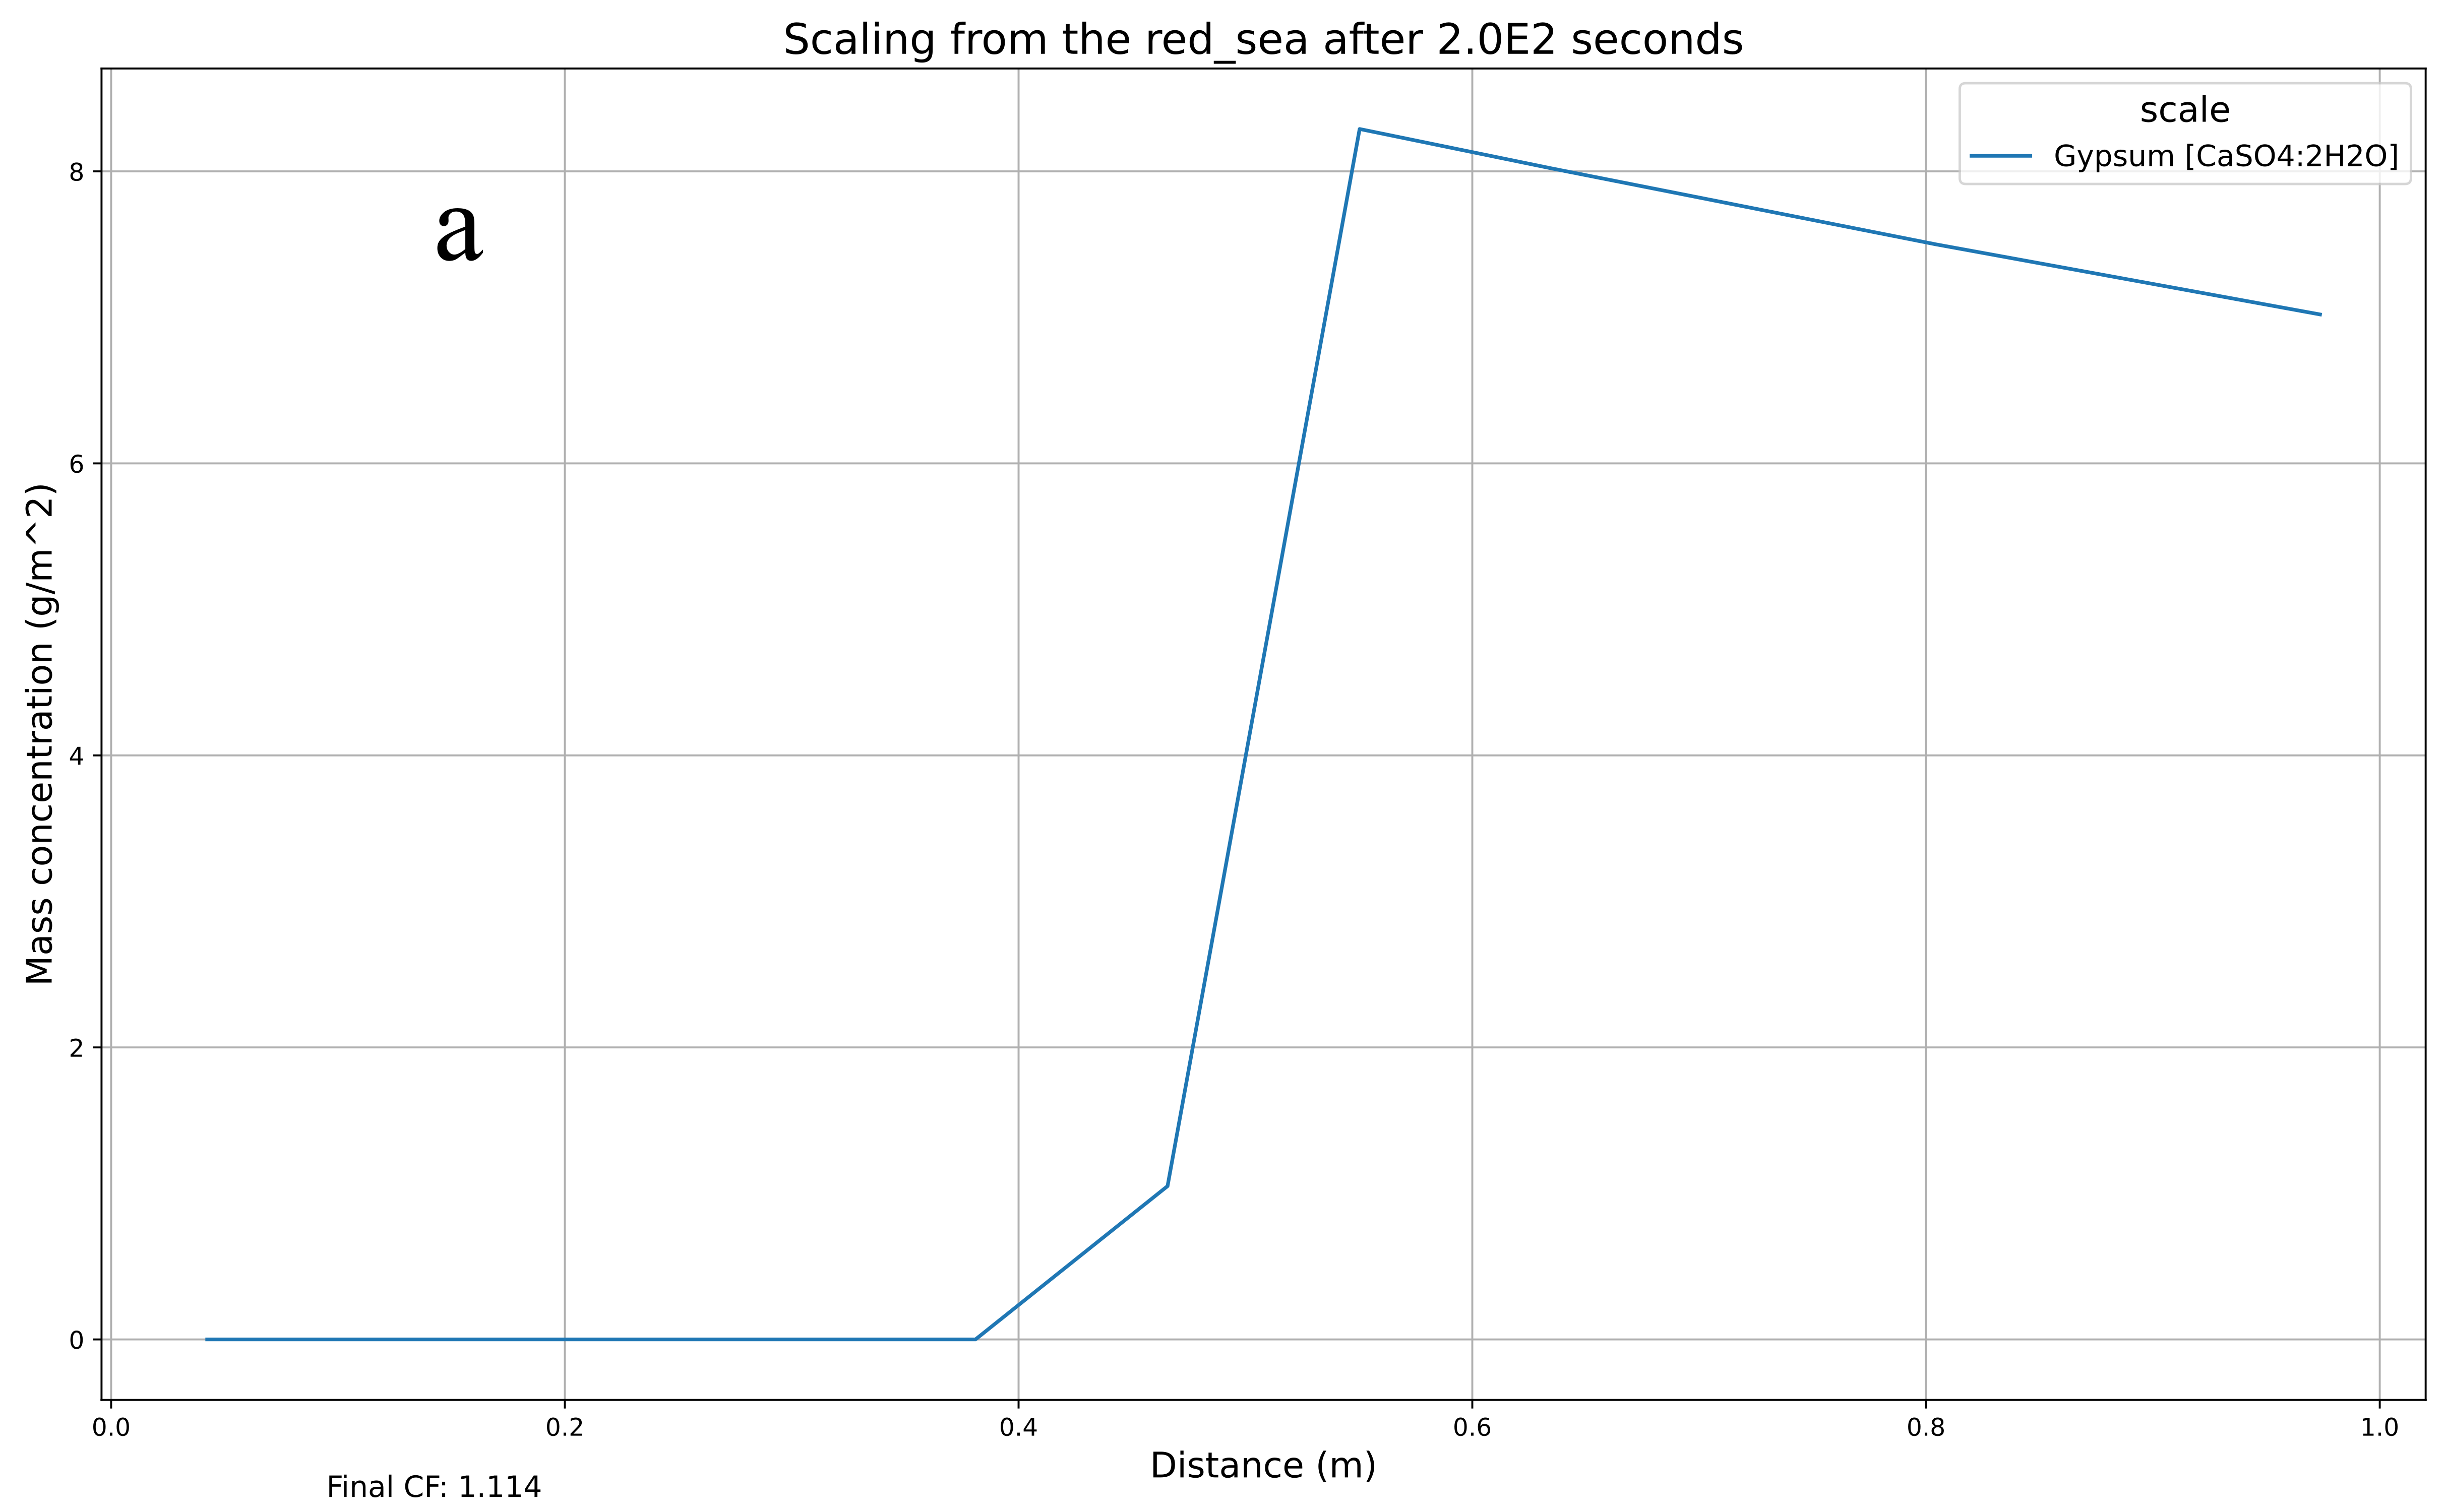
\includegraphics[width=0.9\linewidth]{images/ROSSpy/sensitivity_analyses/permeate_approach/linear_cf.png} \\ \midrule
    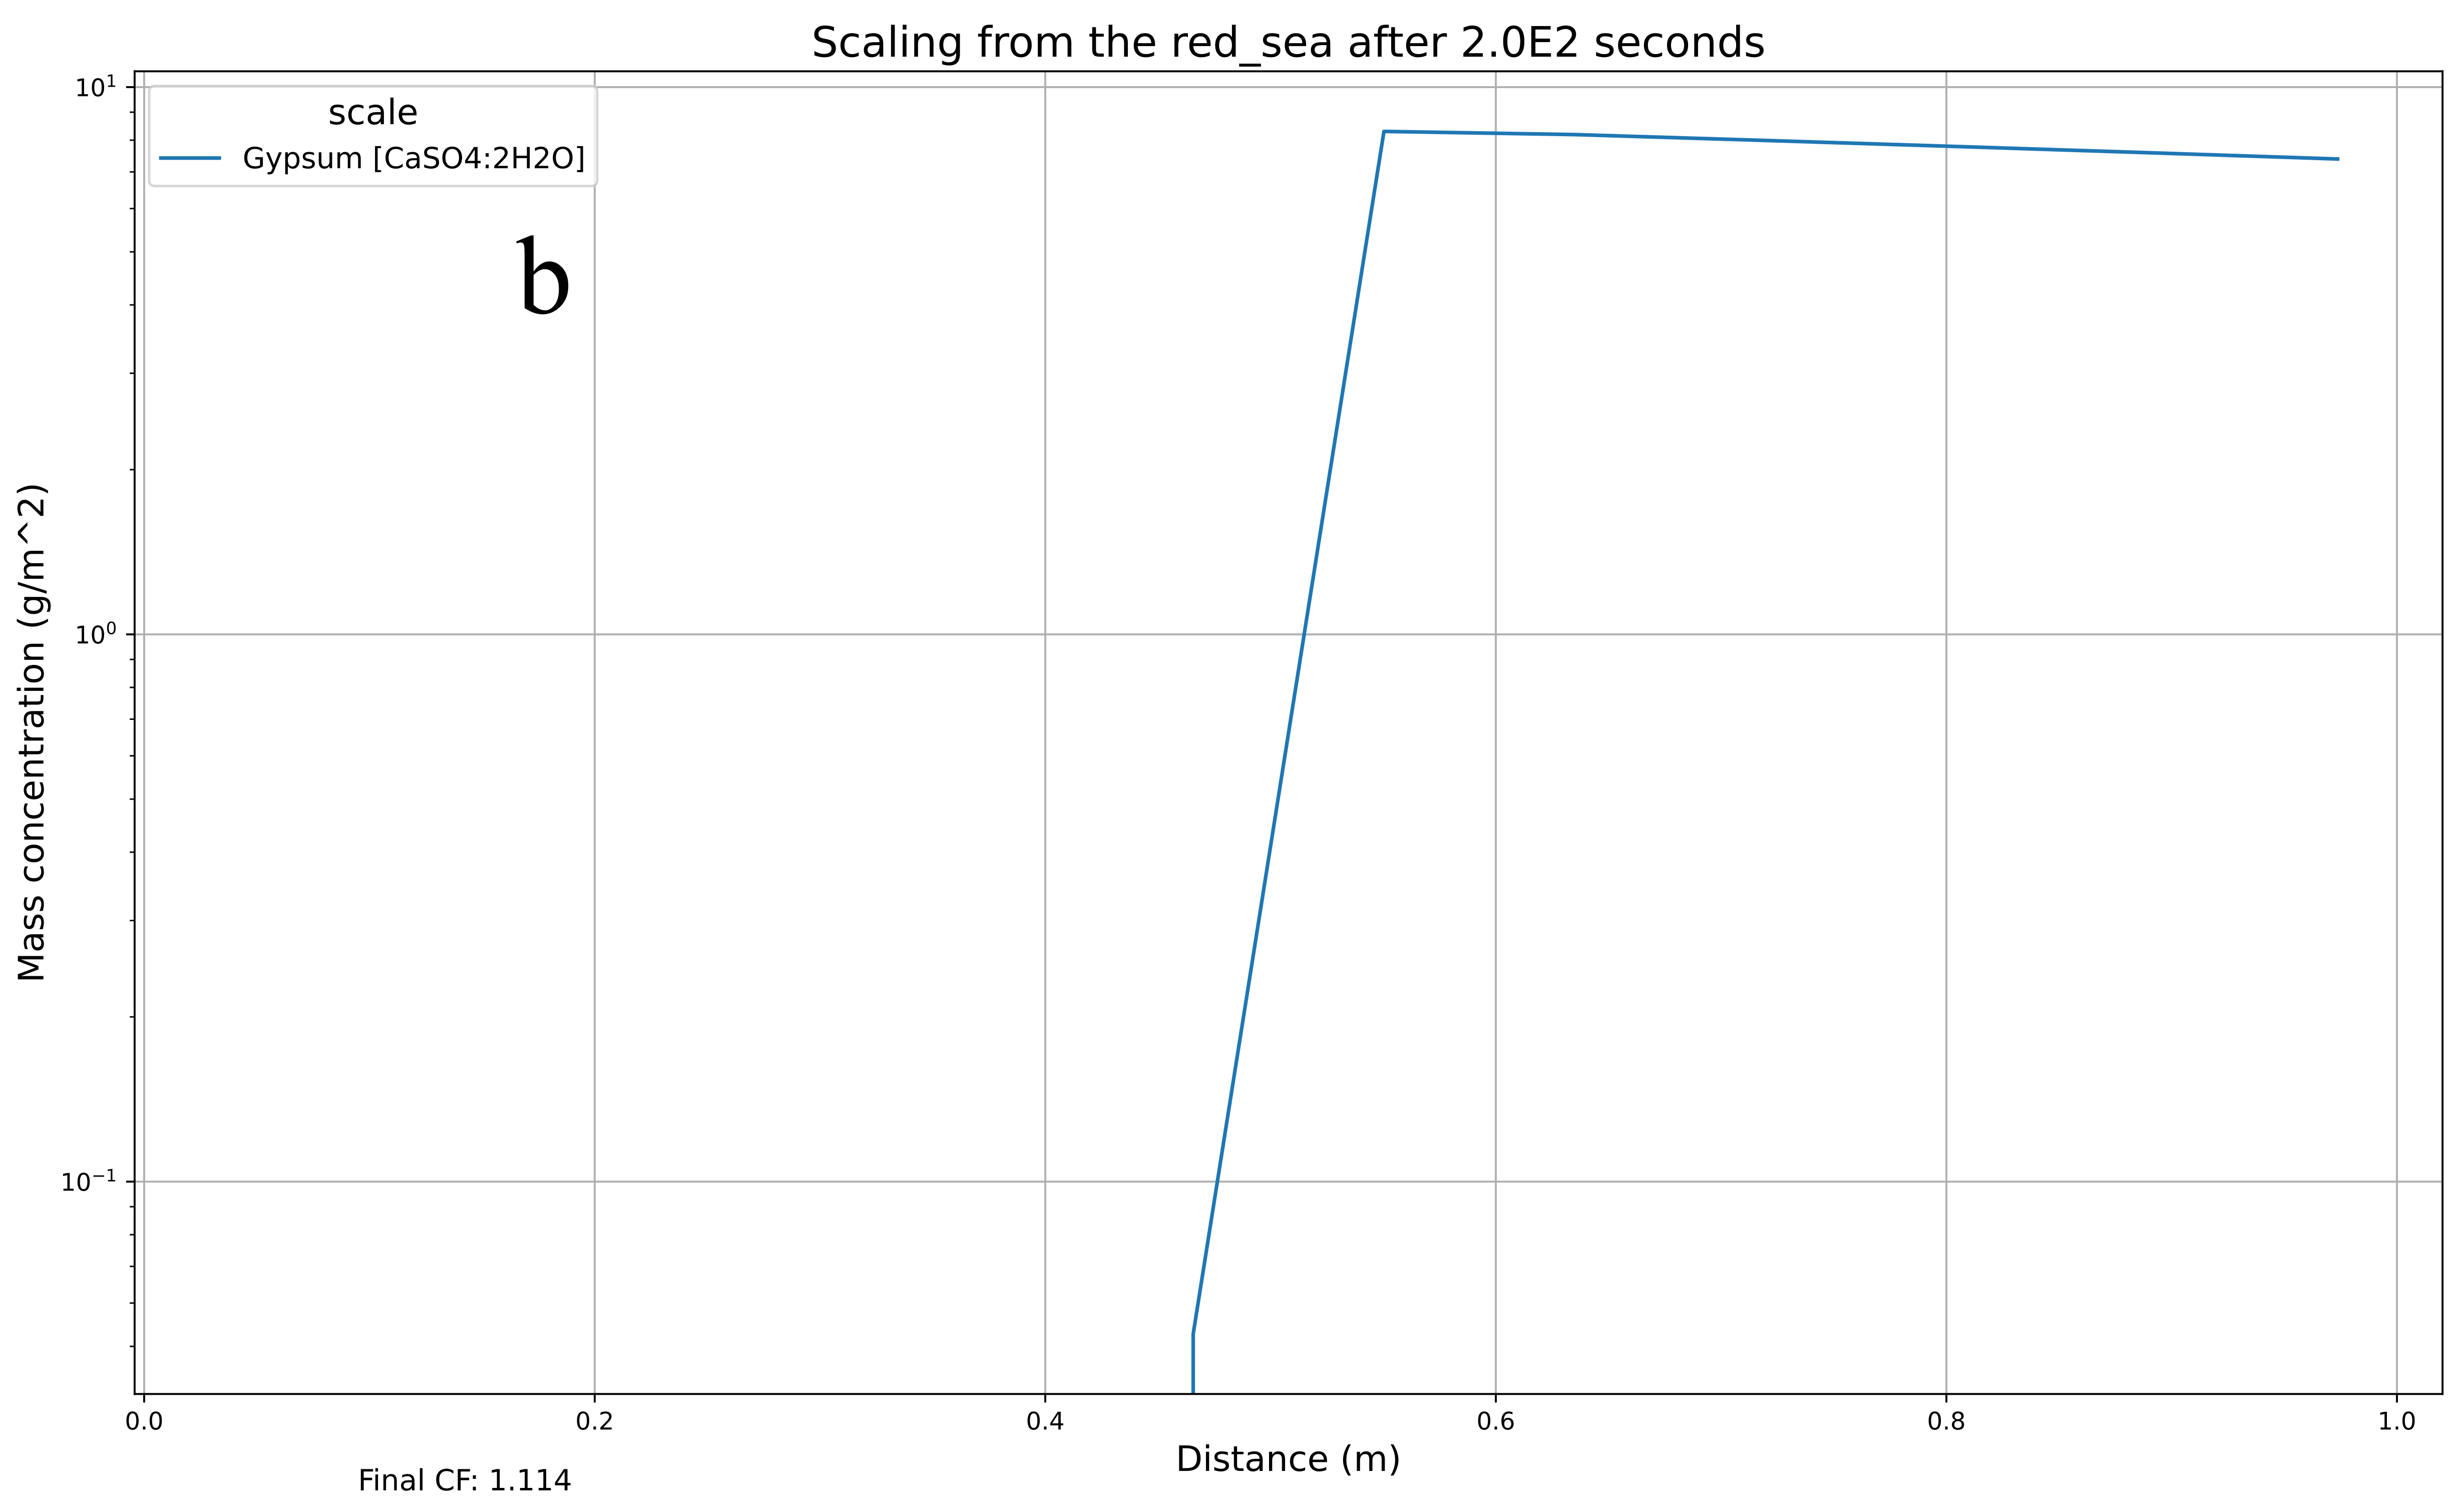
\includegraphics[width=0.9\linewidth]{images/ROSSpy/sensitivity_analyses/permeate_approach/linear_permeate.png} 
    \caption{
        Predicted scaling of the Red Sea at $CF_{effluent}=1.114$ via the a) linear CF and b) linear permeate flux methods. The linear increase in CF of a) slightly homogenizes the distribution of scaling, while the exponential increase in CF of b) skews the distribution of scaling to lesser initially and eventually greater, relative to the linear method of a). These subtle differences in scaling distribution neutralize as the total scaling through both methods are equivalent. 
    }
    \label{permeate_approach}
\end{figure}


\subsubsection{Transport}
The physical transport of feed through the module is simulated in each timestep by 1) migrating the contents of each cell $e$ to the next cell $e+1$; 2) repopulating cell $1$ as new feed solution enters the simulated module; and 3) deleting cell $n$ as brine exits the simulated module. The feed velocity $v_{feed}=\frac{Q_{max~feed}}{A_{feed}}$ is calculated from the maximum feed flowrate $Q_{max~feed}$ ($\frac{m^3}{s}$) and the feed area from \cref{feed_area} of the RO module. Default module parameters in Table S1 are sourced from the DOW FILMTEC BW30-400 RO module, similar to other RO models \cite{Li2012OptimalDesalination}, and supplement user-defined module parameters. The maximum simulation timestep $\Delta t=\frac{l_{cell}}{v_{feed}}$ is calculated according to the Courant Condition \cite{Gnedin2018EnforcingSchemes} ($C_{max}=1 \ge \frac{v_{feed}*t_{max}}{l_{cell}}$) to maintain accurate resolution of the feed flow.

\section{Use cases}
The following sub-sections evince features of our model and its alignment with reported measurements. These studies were conducted through ROSSpy and are available as Python Notebooks in the ROSSpy GitHub repository.

\subsection{CF and Brine formation}
The predicted CF and ionic concentrations of the effluent were verified through comparison with the following three experimental studies, where the reported feed geochemistry and module specifications were parameterized into the model. 

\paragraph{Zaman et al.\cite{Zaman2015DownstreamCompounds}}
This study examines RO brine, from a full-scale water treatment facility in Australia, to understand which minerals are likely to form as scale. The predicted concentrations in Figure \ref{bar_graphs}a were $<6\%-error$ for all but one of the feed ions.

\paragraph{Ahmed et al.\cite{Ahmed2001BrineEmirates}}
This study examines RO brine from 10 small desalination plants in Oman and 8 plants in the United Arab Emirates (UAE) for the purpose of understanding ideal brine disposal methods. We selected the UAE Qidfa I desalination plant from these 18 plants to replicate, since it provided the most comprehensive details. The predicted concentrations in Figure \ref{bar_graphs}b were $<10\%-error$ for all but one of the feed ions. The CF, in the far-right column of Figure \ref{bar_graphs}b, furthermore exhibits a $<1\%-error$, which supports that the reactive transport processes, notably the permeate flux calculations, are accurate.

\paragraph{Hajbi et al.\cite{Hajbi2010ReuseBrine}}
This study  evaluates the recovery of commodity salts from RO brine at a plant in Tunisia. The authors detail specifications of line D -- a polyamide filtration membrane -- in the plant system, in addition to the feed geochemistry, which were all parameterized into our model. The predicted concentrations in Figure \ref{bar_graphs}c were less aligned than the aforementioned two studies, with two ions exceeding $25\%-error$. This is attributed to $40\%$ fewer feed ions being defined by this study, where the incomplete geochemical representation of the feed skews the geochemical calculations of PHREEQC. This is corroborated by the accuracy of the CF prediction in Figure \ref{bar_graphs}c, despite inaccurate concentration predictions, which suggests that the error resides with the geochemical processes and not the reactive transport system. 

\begin{figure}
    \centering
    \begin{tabular}{c|c}
        \multicolumn{2}{c}{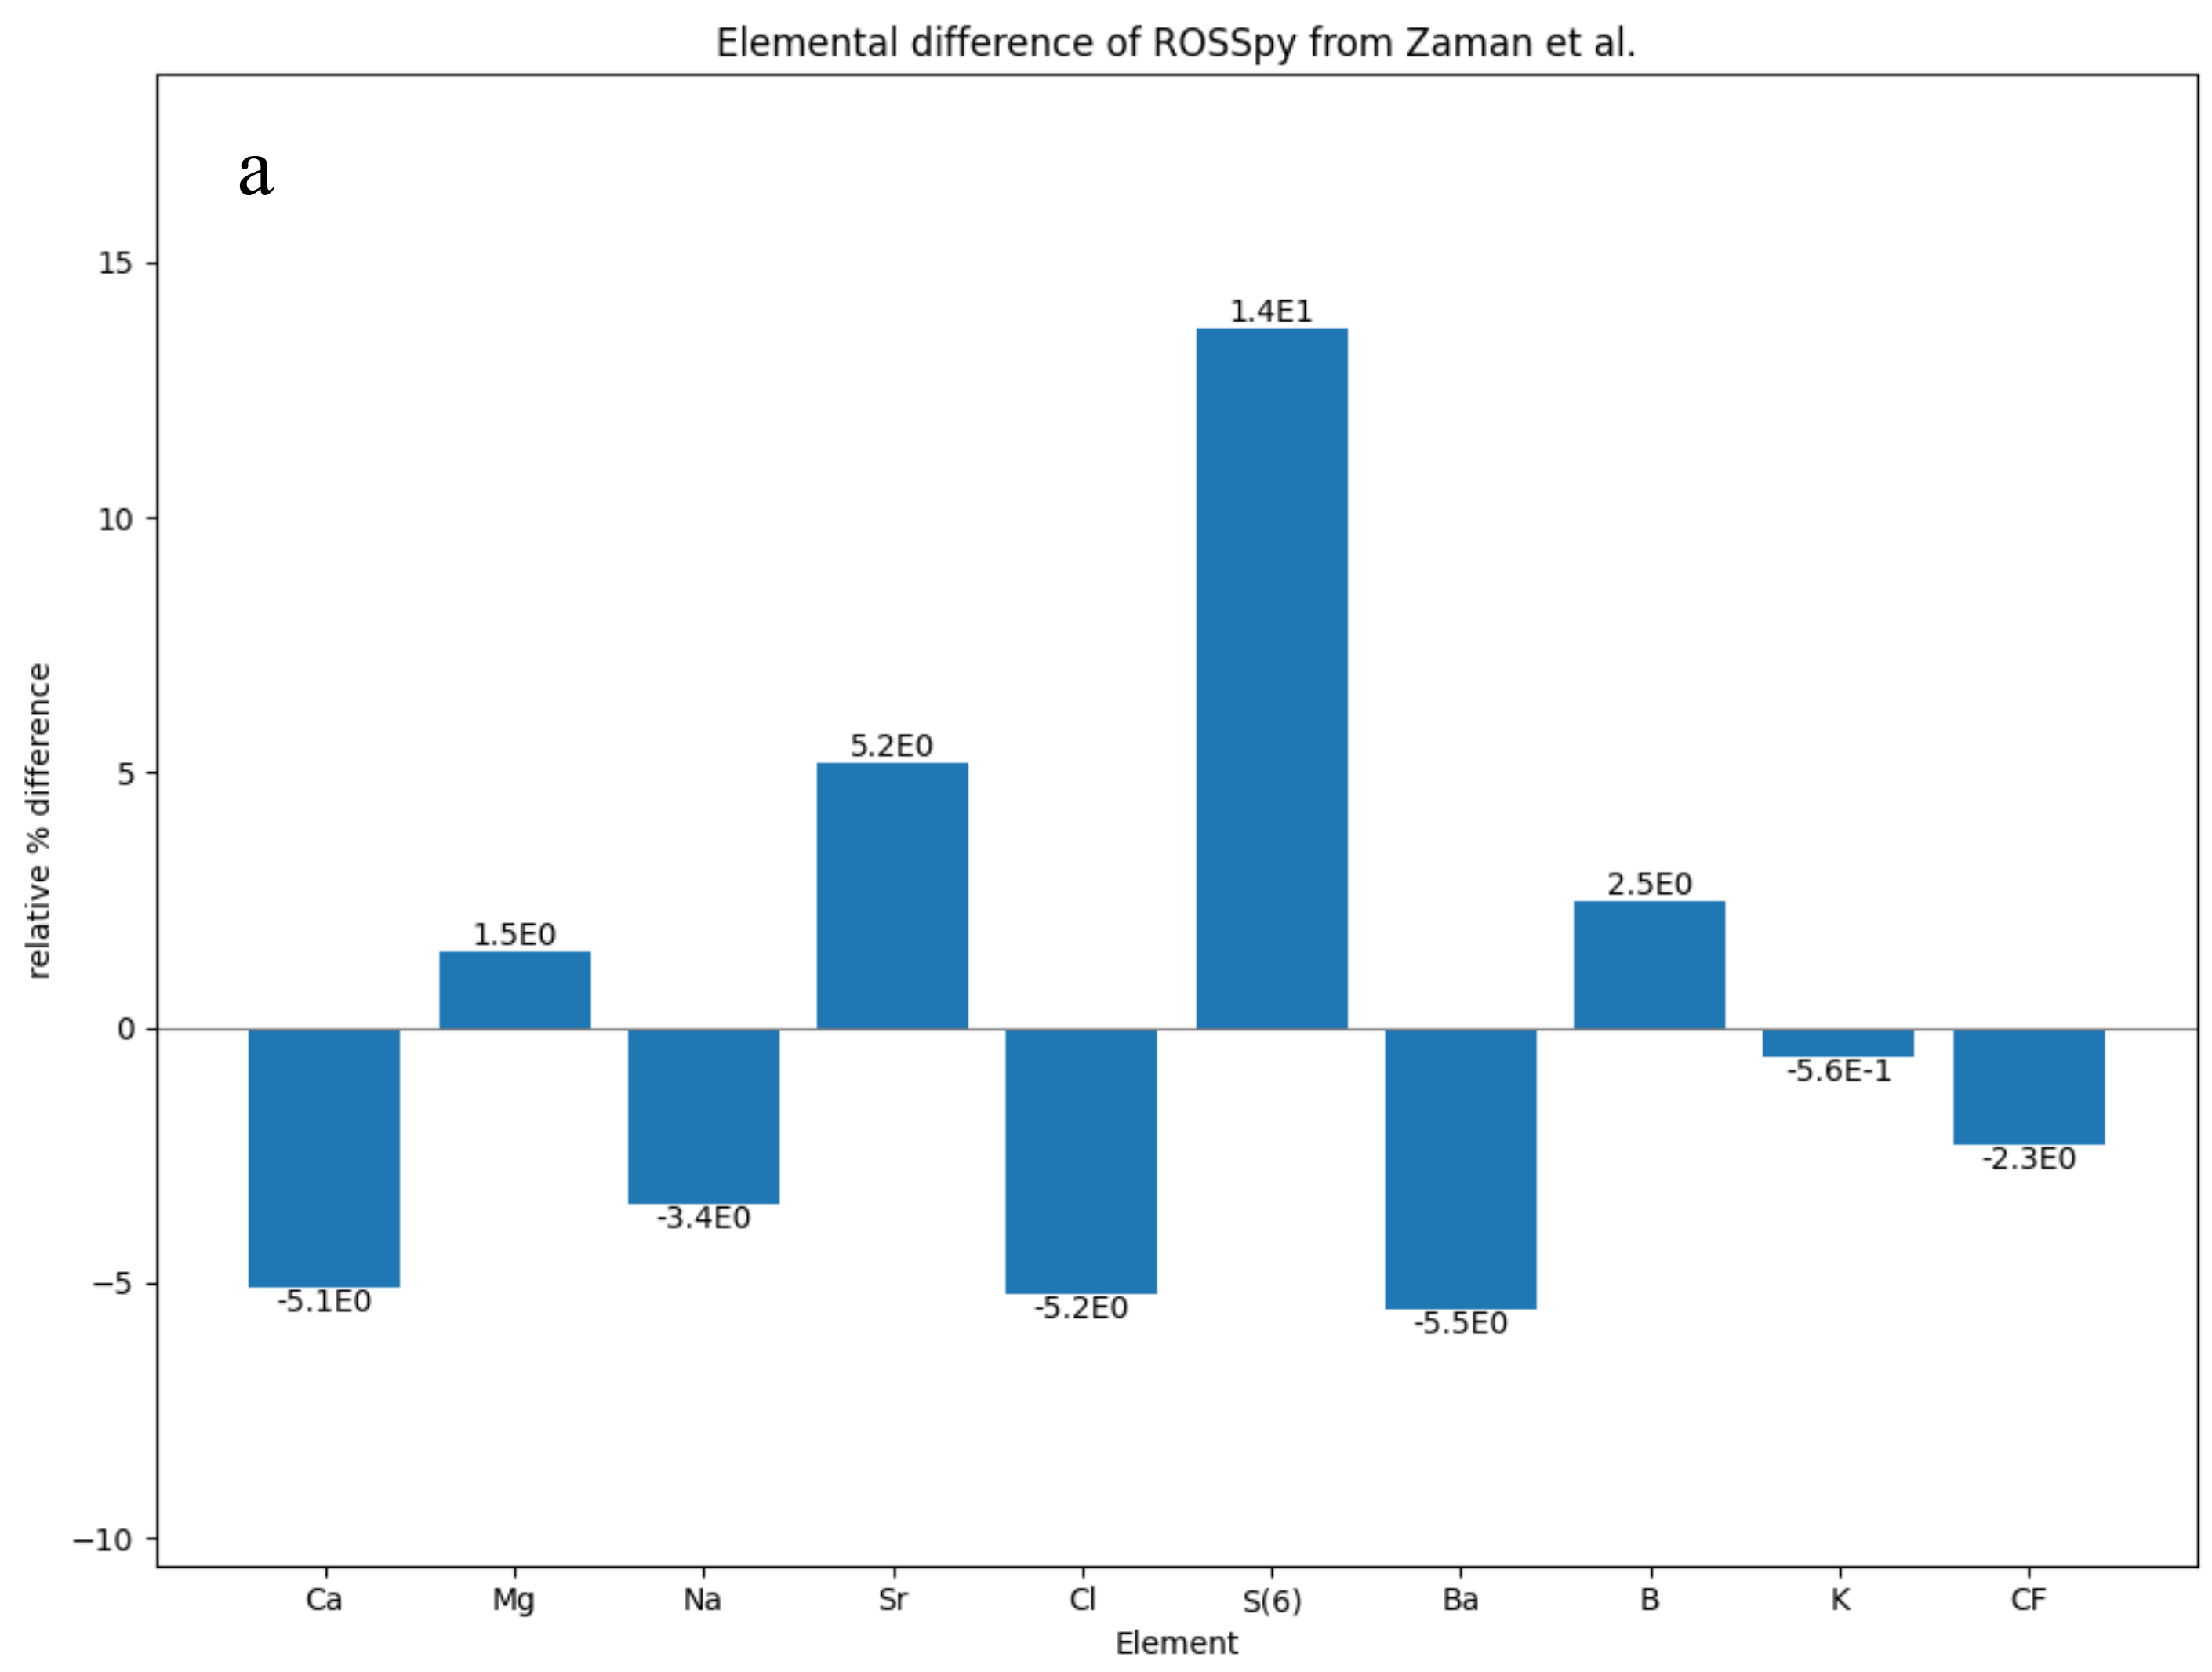
\includegraphics[width=\linewidth]{images/ROSSpy/case_studies/Zaman_comparison.png}} \\ \midrule
        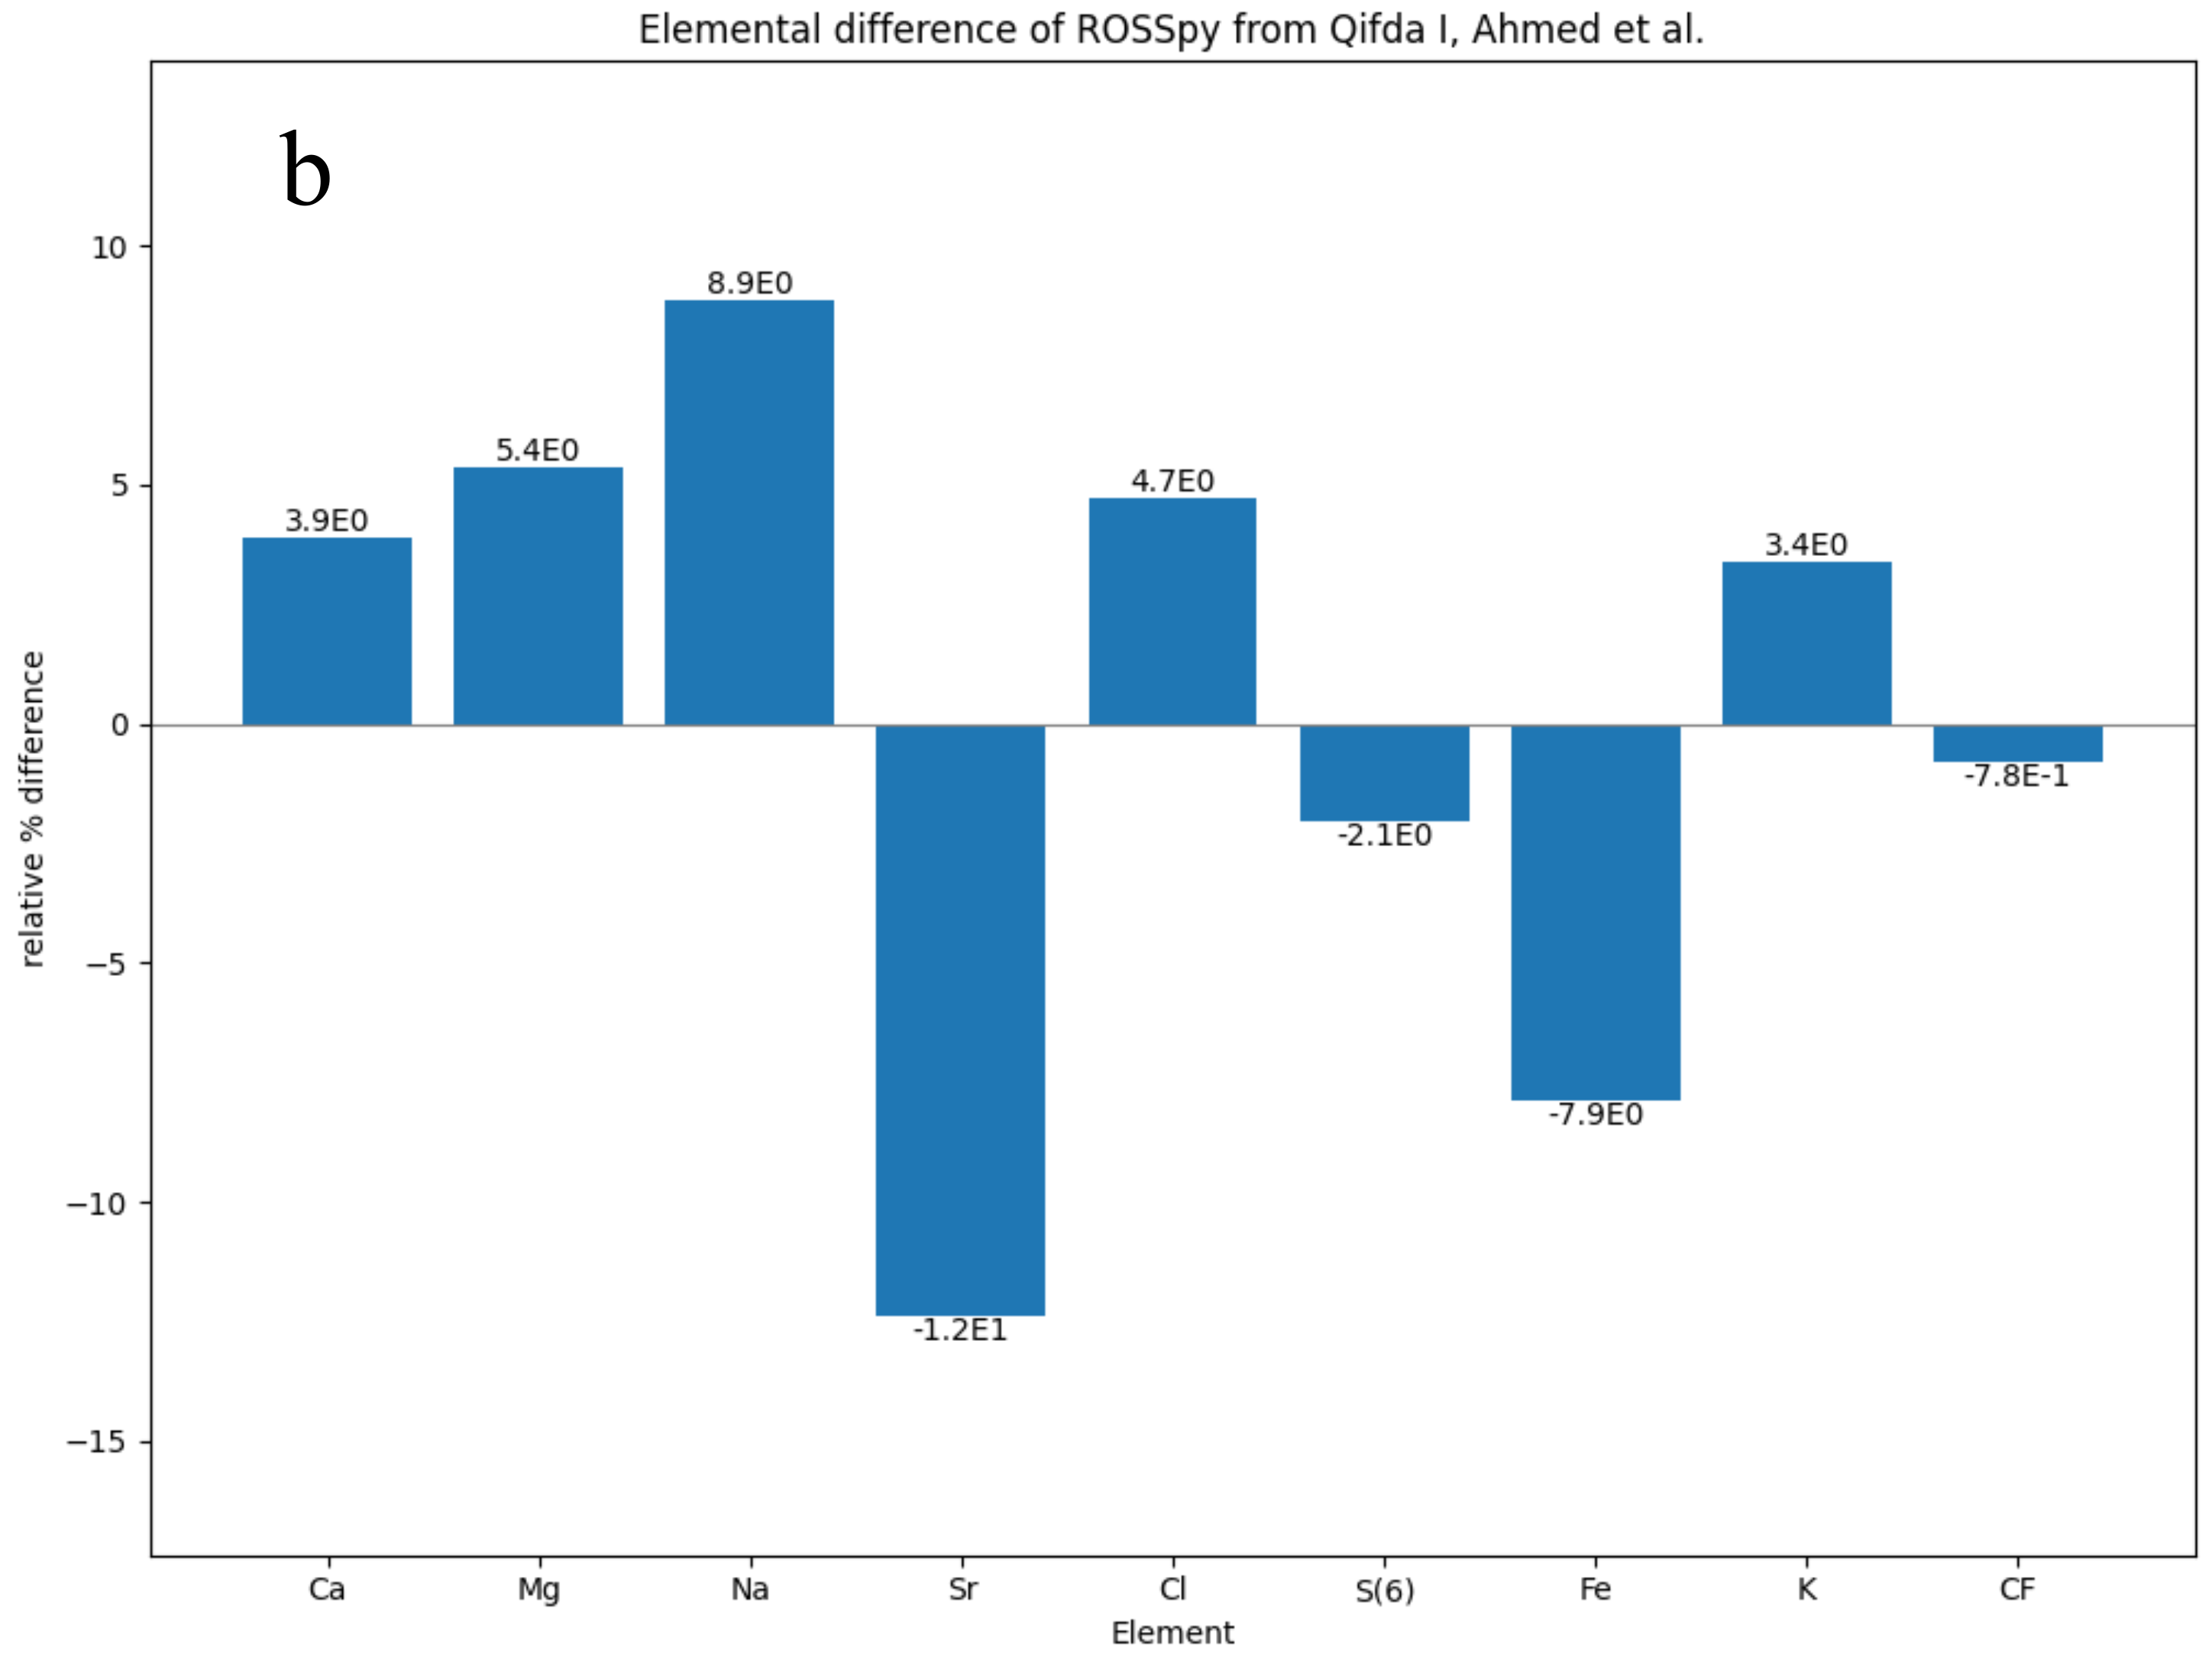
\includegraphics[width=0.49\linewidth]{images/ROSSpy/case_studies/Ahmed_comparison.png} & 
        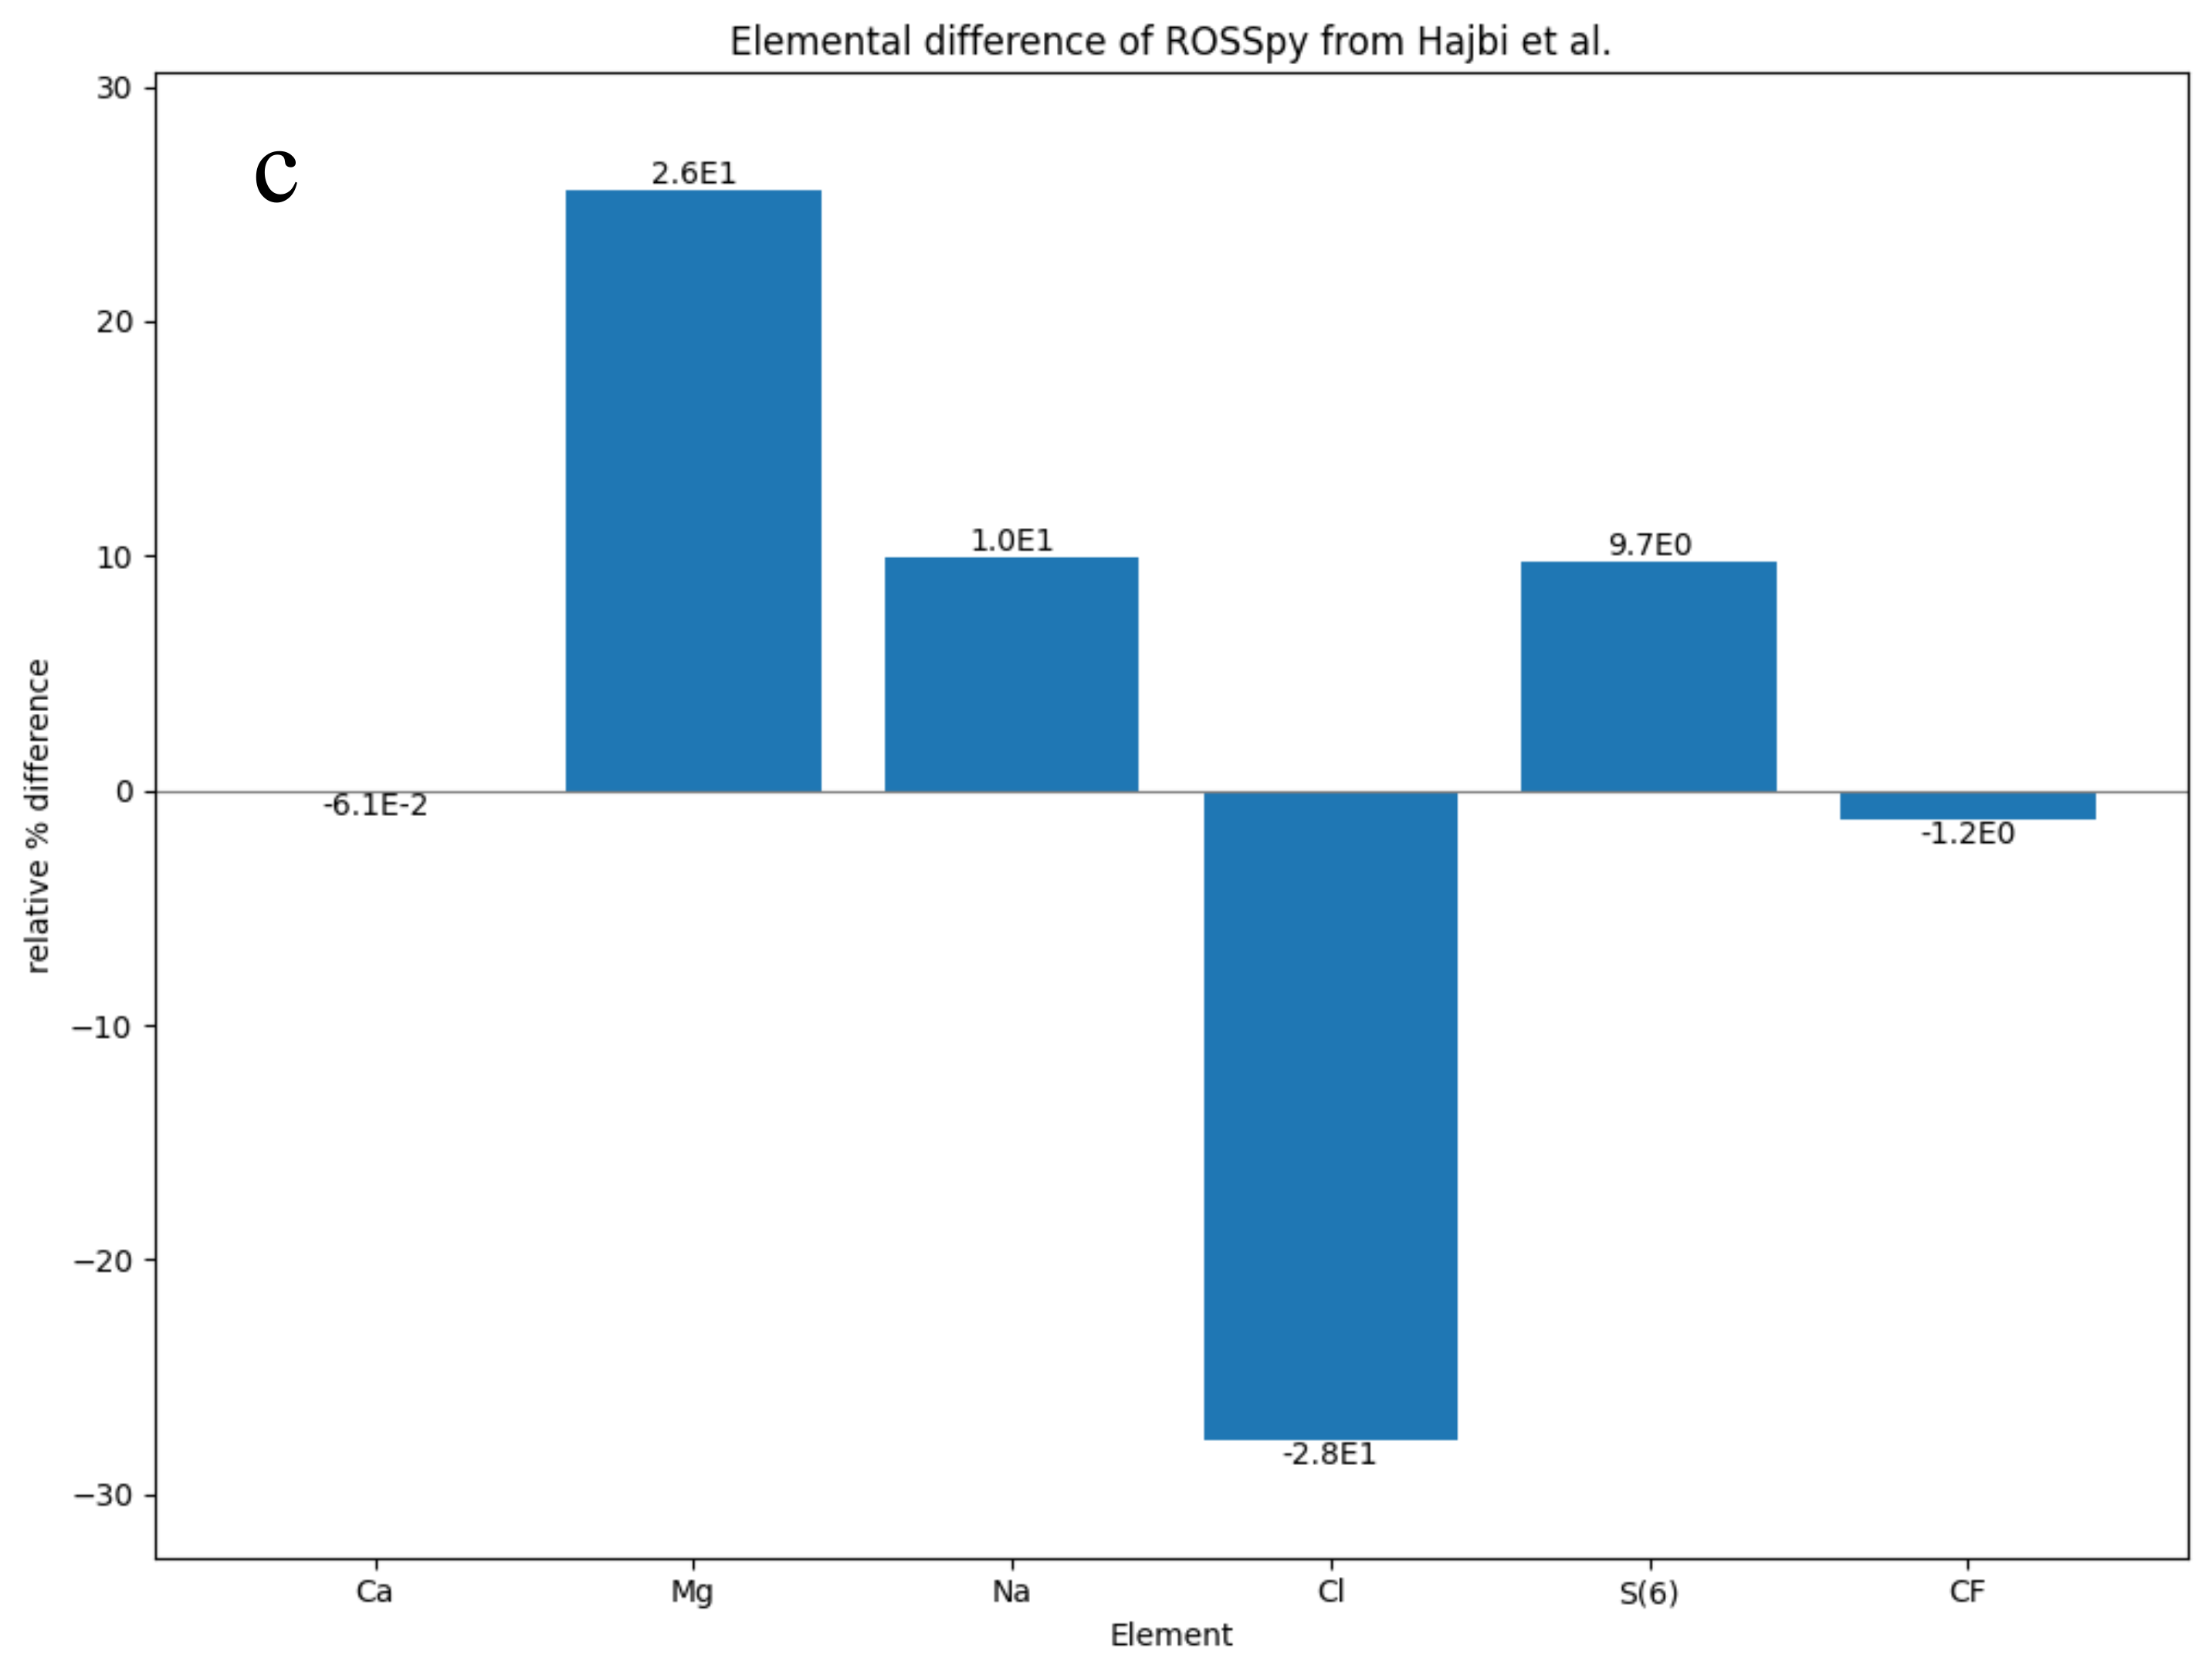
\includegraphics[width=0.49\linewidth]{images/ROSSpy/case_studies/Hajbi_comparison.png} \\ \bottomrule
    \end{tabular}
    \caption{
        The \%-error between predicted and experimental brine concentrations from RO plants. Panels a-c) correspond to comparisons with the Zaman et al. \cite{Zaman2015DownstreamCompounds}, Ahmed et al. \cite{Ahmed2001BrineEmirates}, and Hajbi et al. \cite{Hajbi2010ReuseBrine} studies, respectively, and each possess different y-axis scales to best resolve the bars in each graph. The trend is that prediction accuracy is proportional to the quantity of parameterized ions. 
    }
    \label{bar_graphs}
\end{figure}


\subsection{Scaling}
The scaling predictions were verified qualitatively from experimental literature and quantitatively from theoretical calculations, since experimental literature that quantified scalants with feed geochemistry was not discovered.

\subsubsection{Quantitative}
The quantitative verification consisted of two simple cases of Gypsum precipitation. 1) The first case in Table \ref{gypsum_ice_table} consists of a solution with only $Ca^{2+}$ and $SO_4^{2-}$, where the ionic concentrations decreased by $0.01859$ moles while $0.01961$ moles of Gypsum precipitated. This 5\% discrepancy in mass balance is attributed to the printed PHREEQC values in this calculation neglecting diffusion within the feed solution, yet diffusion is considered in the final output of PHREEQC. 2) The second case in Table S1 evaluates Gypsum precipitation from desalinating the solution from the first case with that from the Red Sea, which only precipitates Gypsum in our model. The simple solution precipitated $0.181$ moles of Gypsum, while the Red Sea precipitated $0.194$ moles. This $+7\%$-error is attributed to ionic interactions within the Red Sea feed that are not present by the simple solution of only $Ca^{2+}$ and $SO_4^{2-}$. These subtle $[5,7]\%$ deviations, even without considering the coarse assumptions in these simple examples, are relatively minor in the context of other sources of error, such as feed measurements, and still elicit quantitative consistency in scaling predictions.

\begin{table}
    \centering
    \begin{tabular}{c|ccccc}
      \toprule
       & $Ca^{2+}$ & $+$ & $SO_4^{2-}$ & $\leftrightharpoons$ & $CaSO_4$ \\
      \midrule
      I & $0.3545$ && $1.816$ && $0$ \\
      C & $-0.01859$ && $-0.01859$ && $+0.01961$ \\
      F & $0.3360$ && $1.797$ && $0.01961$ \\
      \bottomrule
    \end{tabular}
    \caption{
        Gypsum precipitation according to the ICE (Initial, Change, Equilibrium) framework, except that "Equilibrium" (E) is replaced with "Final" (F) since the system does not completely reach equilibrium within the RO module. The $5\%-error$ in row C, between the changes in ionic and Gypsum moles, suggests a subtle discrepancy in mass balance of PHREEQC; however, this is attributed to PHREEQC printing values before diffusion is incorporated in the calculations, per David Parkhurst. 
      }
    \label{gypsum_ice_table}
\end{table}

\subsubsection{Qualitative}
The scaling predictions were qualitatively verified through three experimental studies. 

\paragraph{Karabelas et al., 2020 \cite{Karabelas2020ScalingTools}}
This study inspired features of ROSSpy by reviewing the state-of-the-art, and future directions, for predictive scaling software. The study also, importantly, describes in its Supporting Information scalants that were observed after desalination with defined conditions. Scaling predictions from these conditions in Figure \ref{qualitative_scaling}a, over a few PHREEQC databases, match the reported scalants ("Calcite but not Gypsum" and a "few other salts, such as Barite and Dolomite, could also deposit at downstream...") in numerous aspects: 1) Calcite was the primary scalant; 2) Gypsum was not observed; 3) a few other salts precipitated, including Dolomite and Barite, depending upon the PHREEQC database; and 4) these other salts precipitated primarily in the downstream portion of the module.  

\paragraph{Karabelas et al., 2014 \cite{Karabelas2014IncipientChannels}}
This study elucidates the mechanisms of incipient scaling from RO desalination -- with Gypsum as the archetypal scalant \cite{Lyster2009CoupledModule}. The ID 28SC trial, which was the most thoroughly described trial, was simulated and Gypsum was the only predicted scalant in Figure \ref{qualitative_scaling}b, just as the reported scalant.  

\paragraph{Lee et al., 2009 \cite{Lee2009MembraneWastewater}}
This study evaluates the use of a membrane bioreactor -- a hollow-fiber membrane module design that is mechanistically similar to RO and thus can be represented by our model -- to treat wastewater. The wastewater filtration system was simulated, and the only predicted scalant was Calcite in Figure \ref{qualitative_scaling}c, just as the reported scalant.

\begin{figure}
    \begin{tabular}{c|c}
        \multicolumn{2}{c}{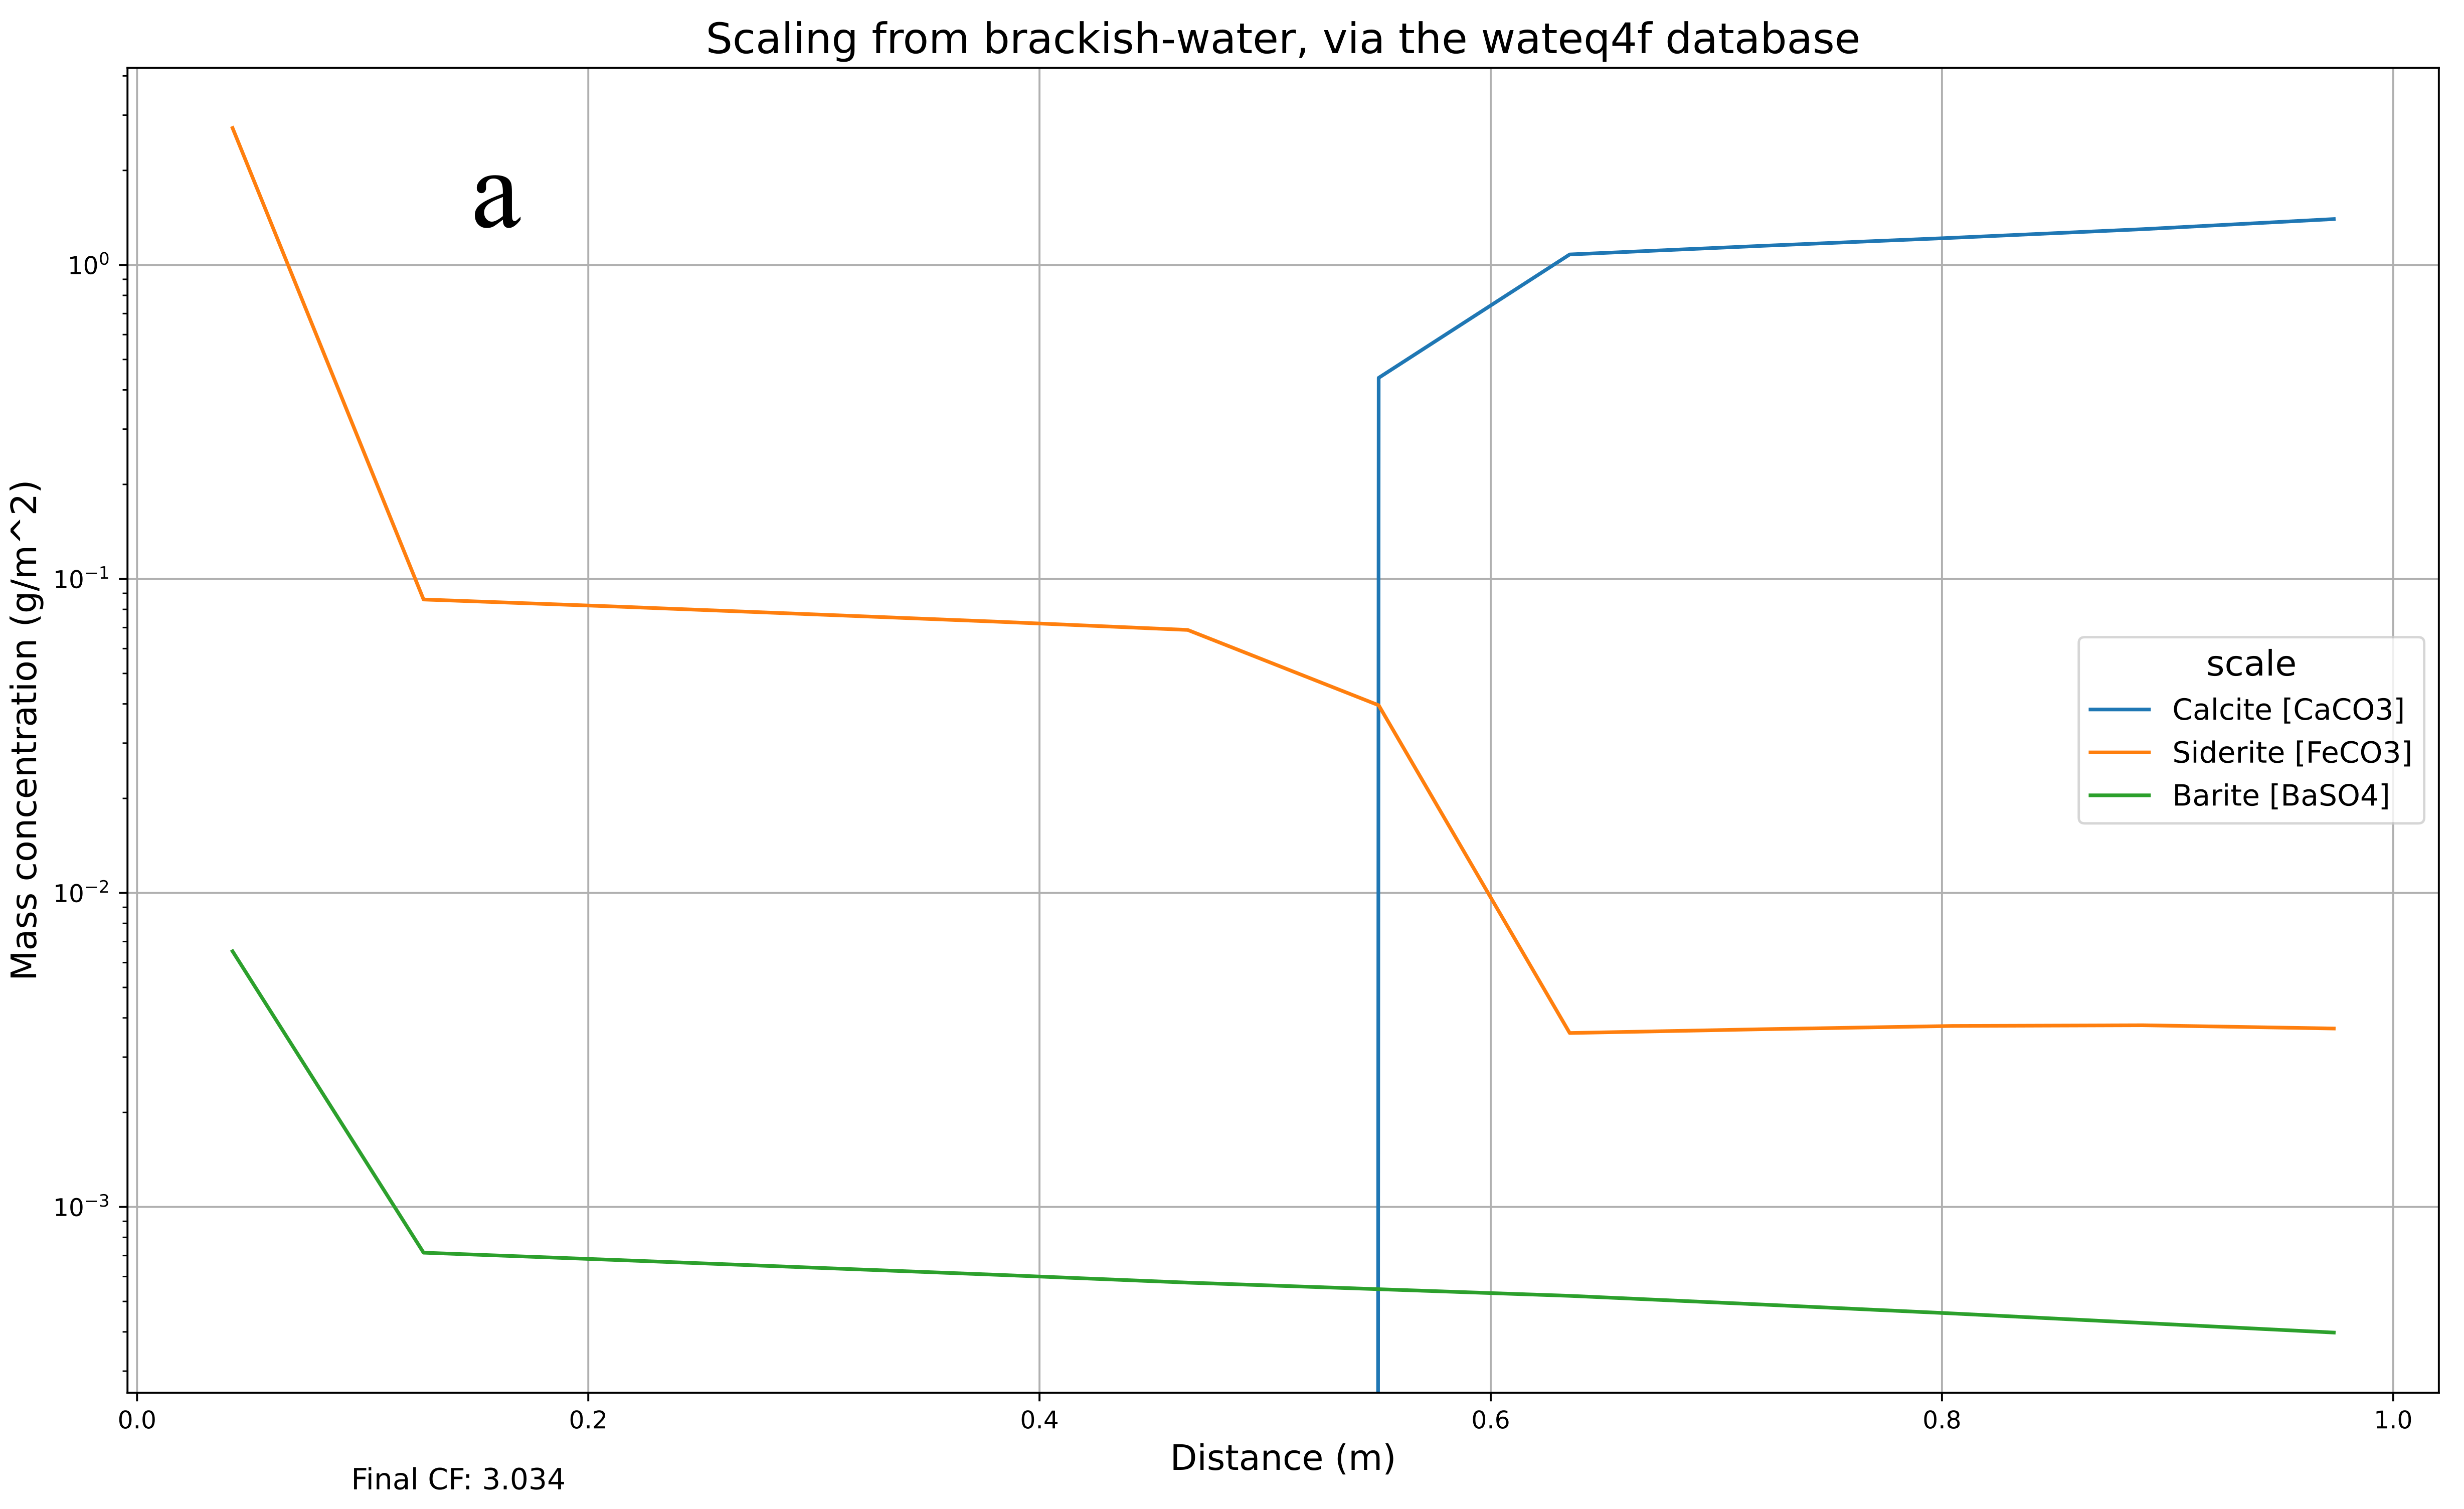
\includegraphics[width=\linewidth]{images/ROSSpy/case_studies/Karabelas_2020_wateq4f.png}} \\
        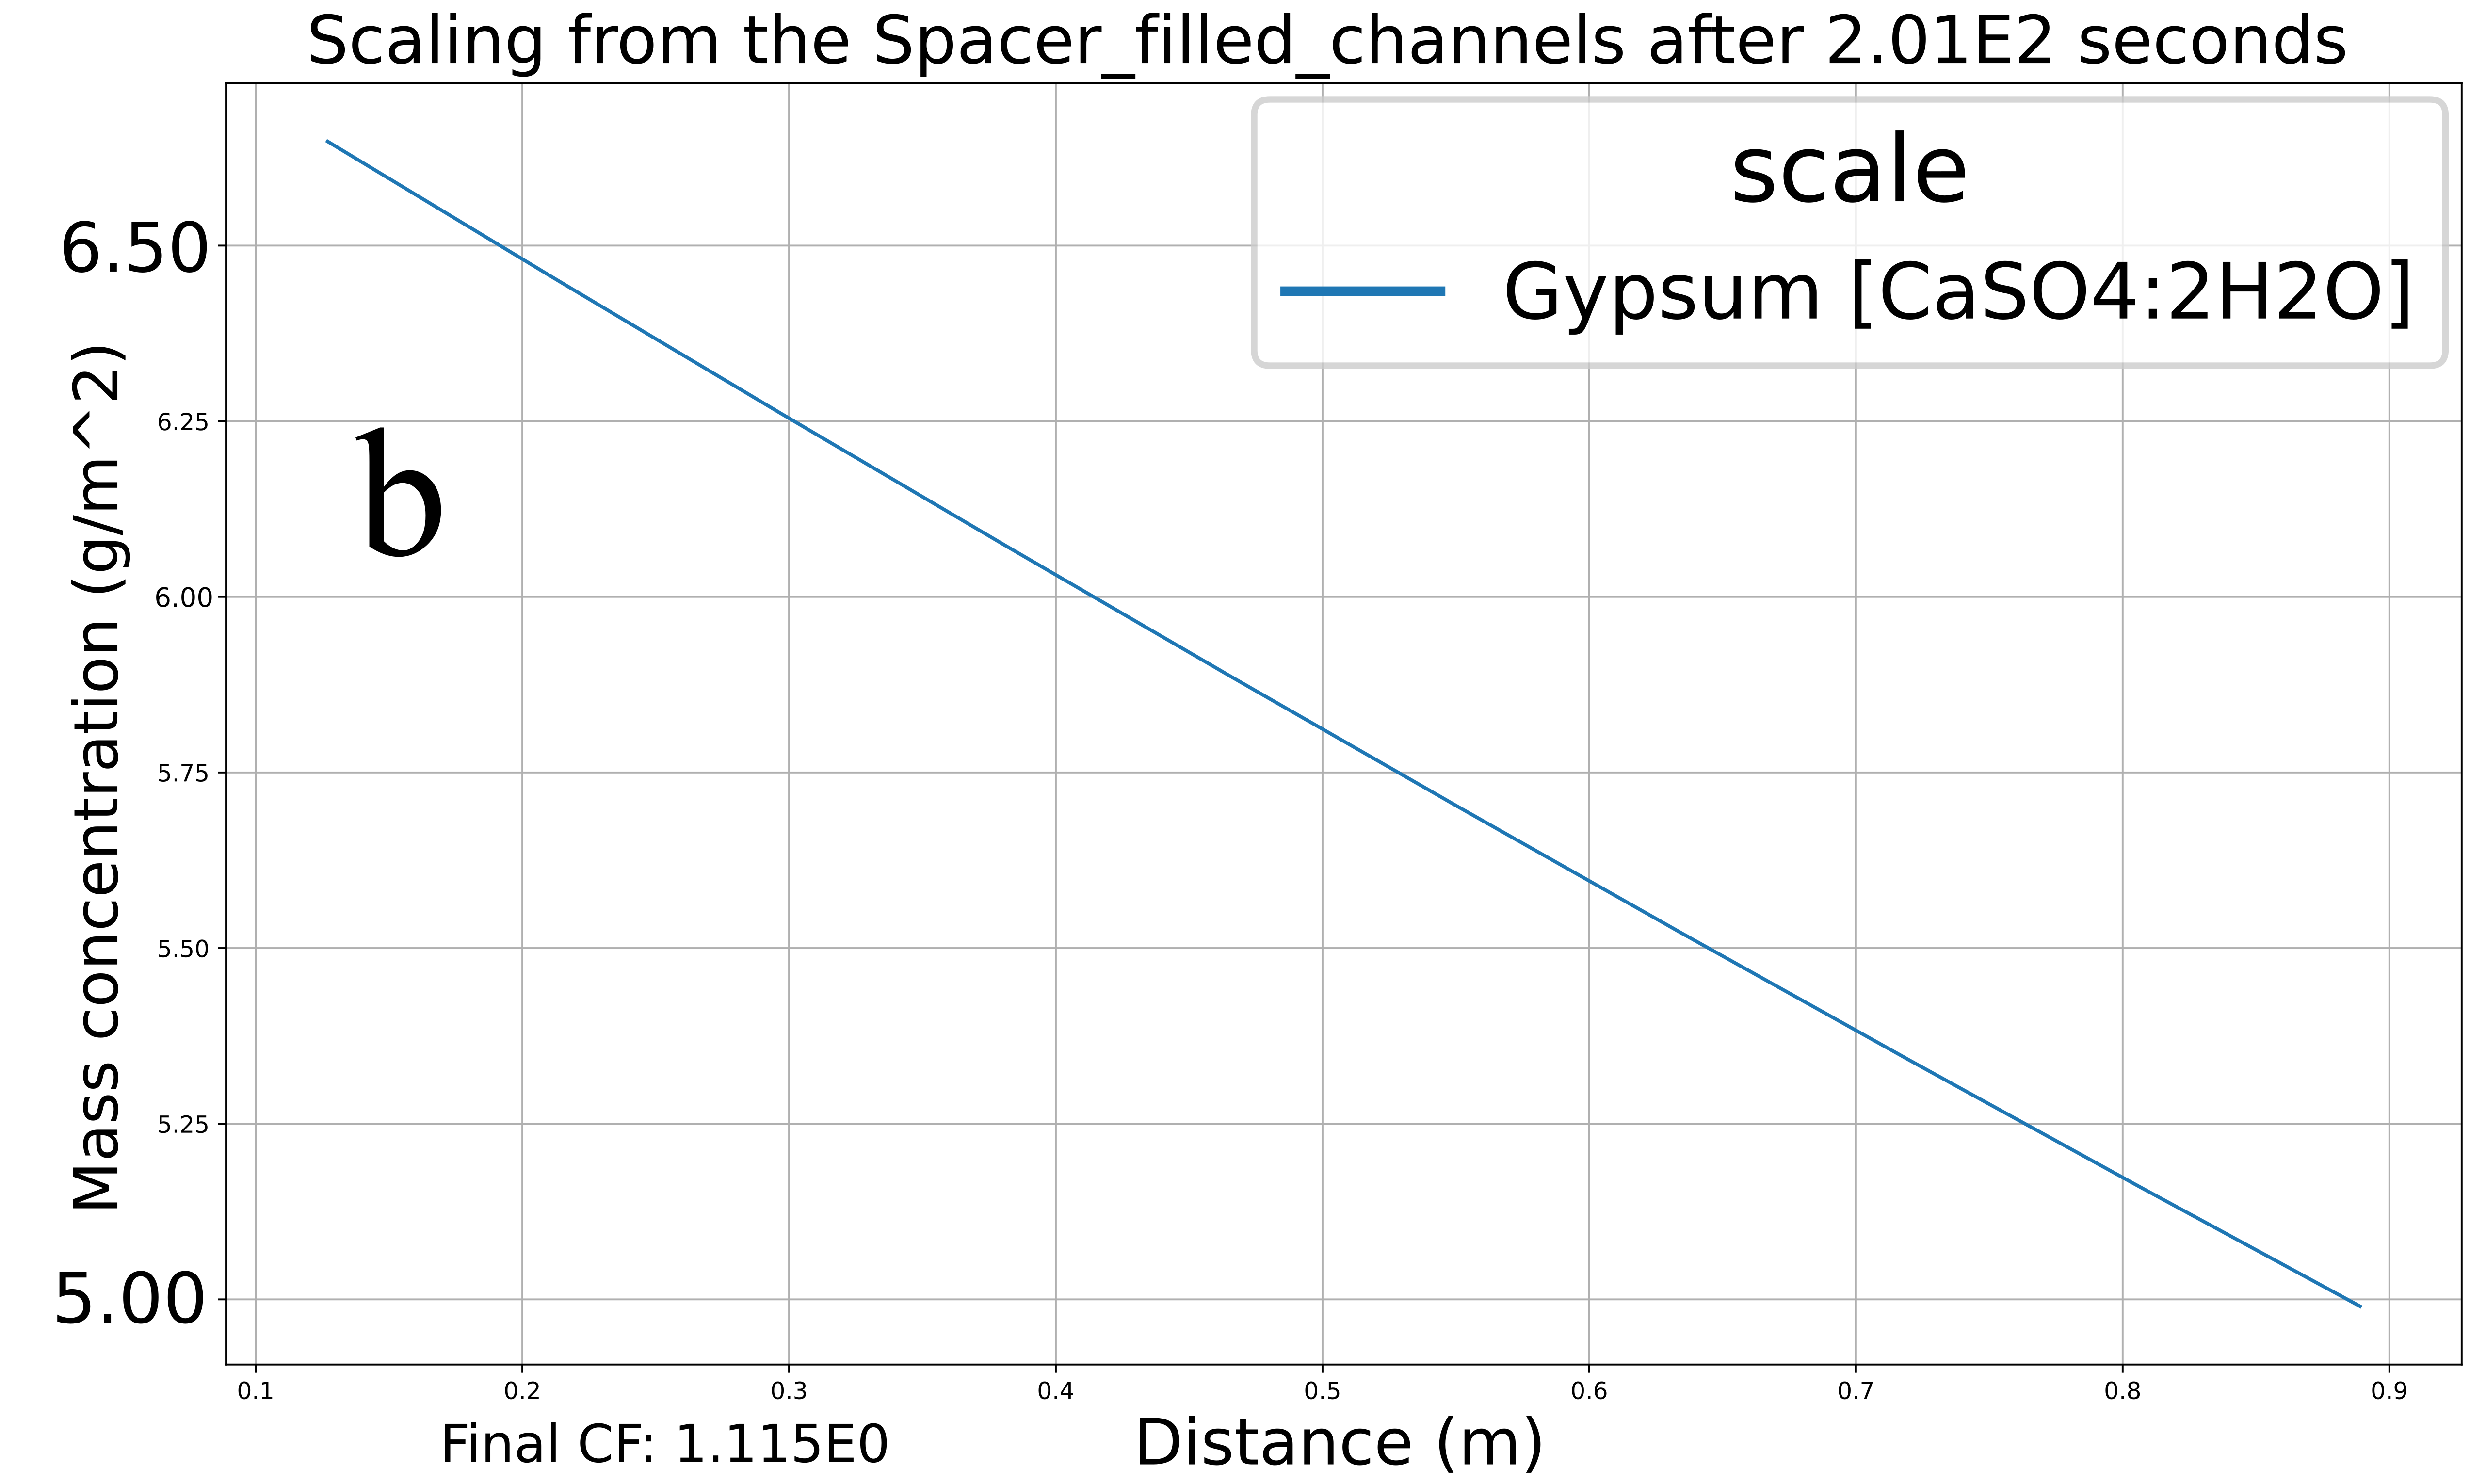
\includegraphics[width=0.49\linewidth]{images/ROSSpy/case_studies/Karabelas_2014_pitzer.png} 
        & 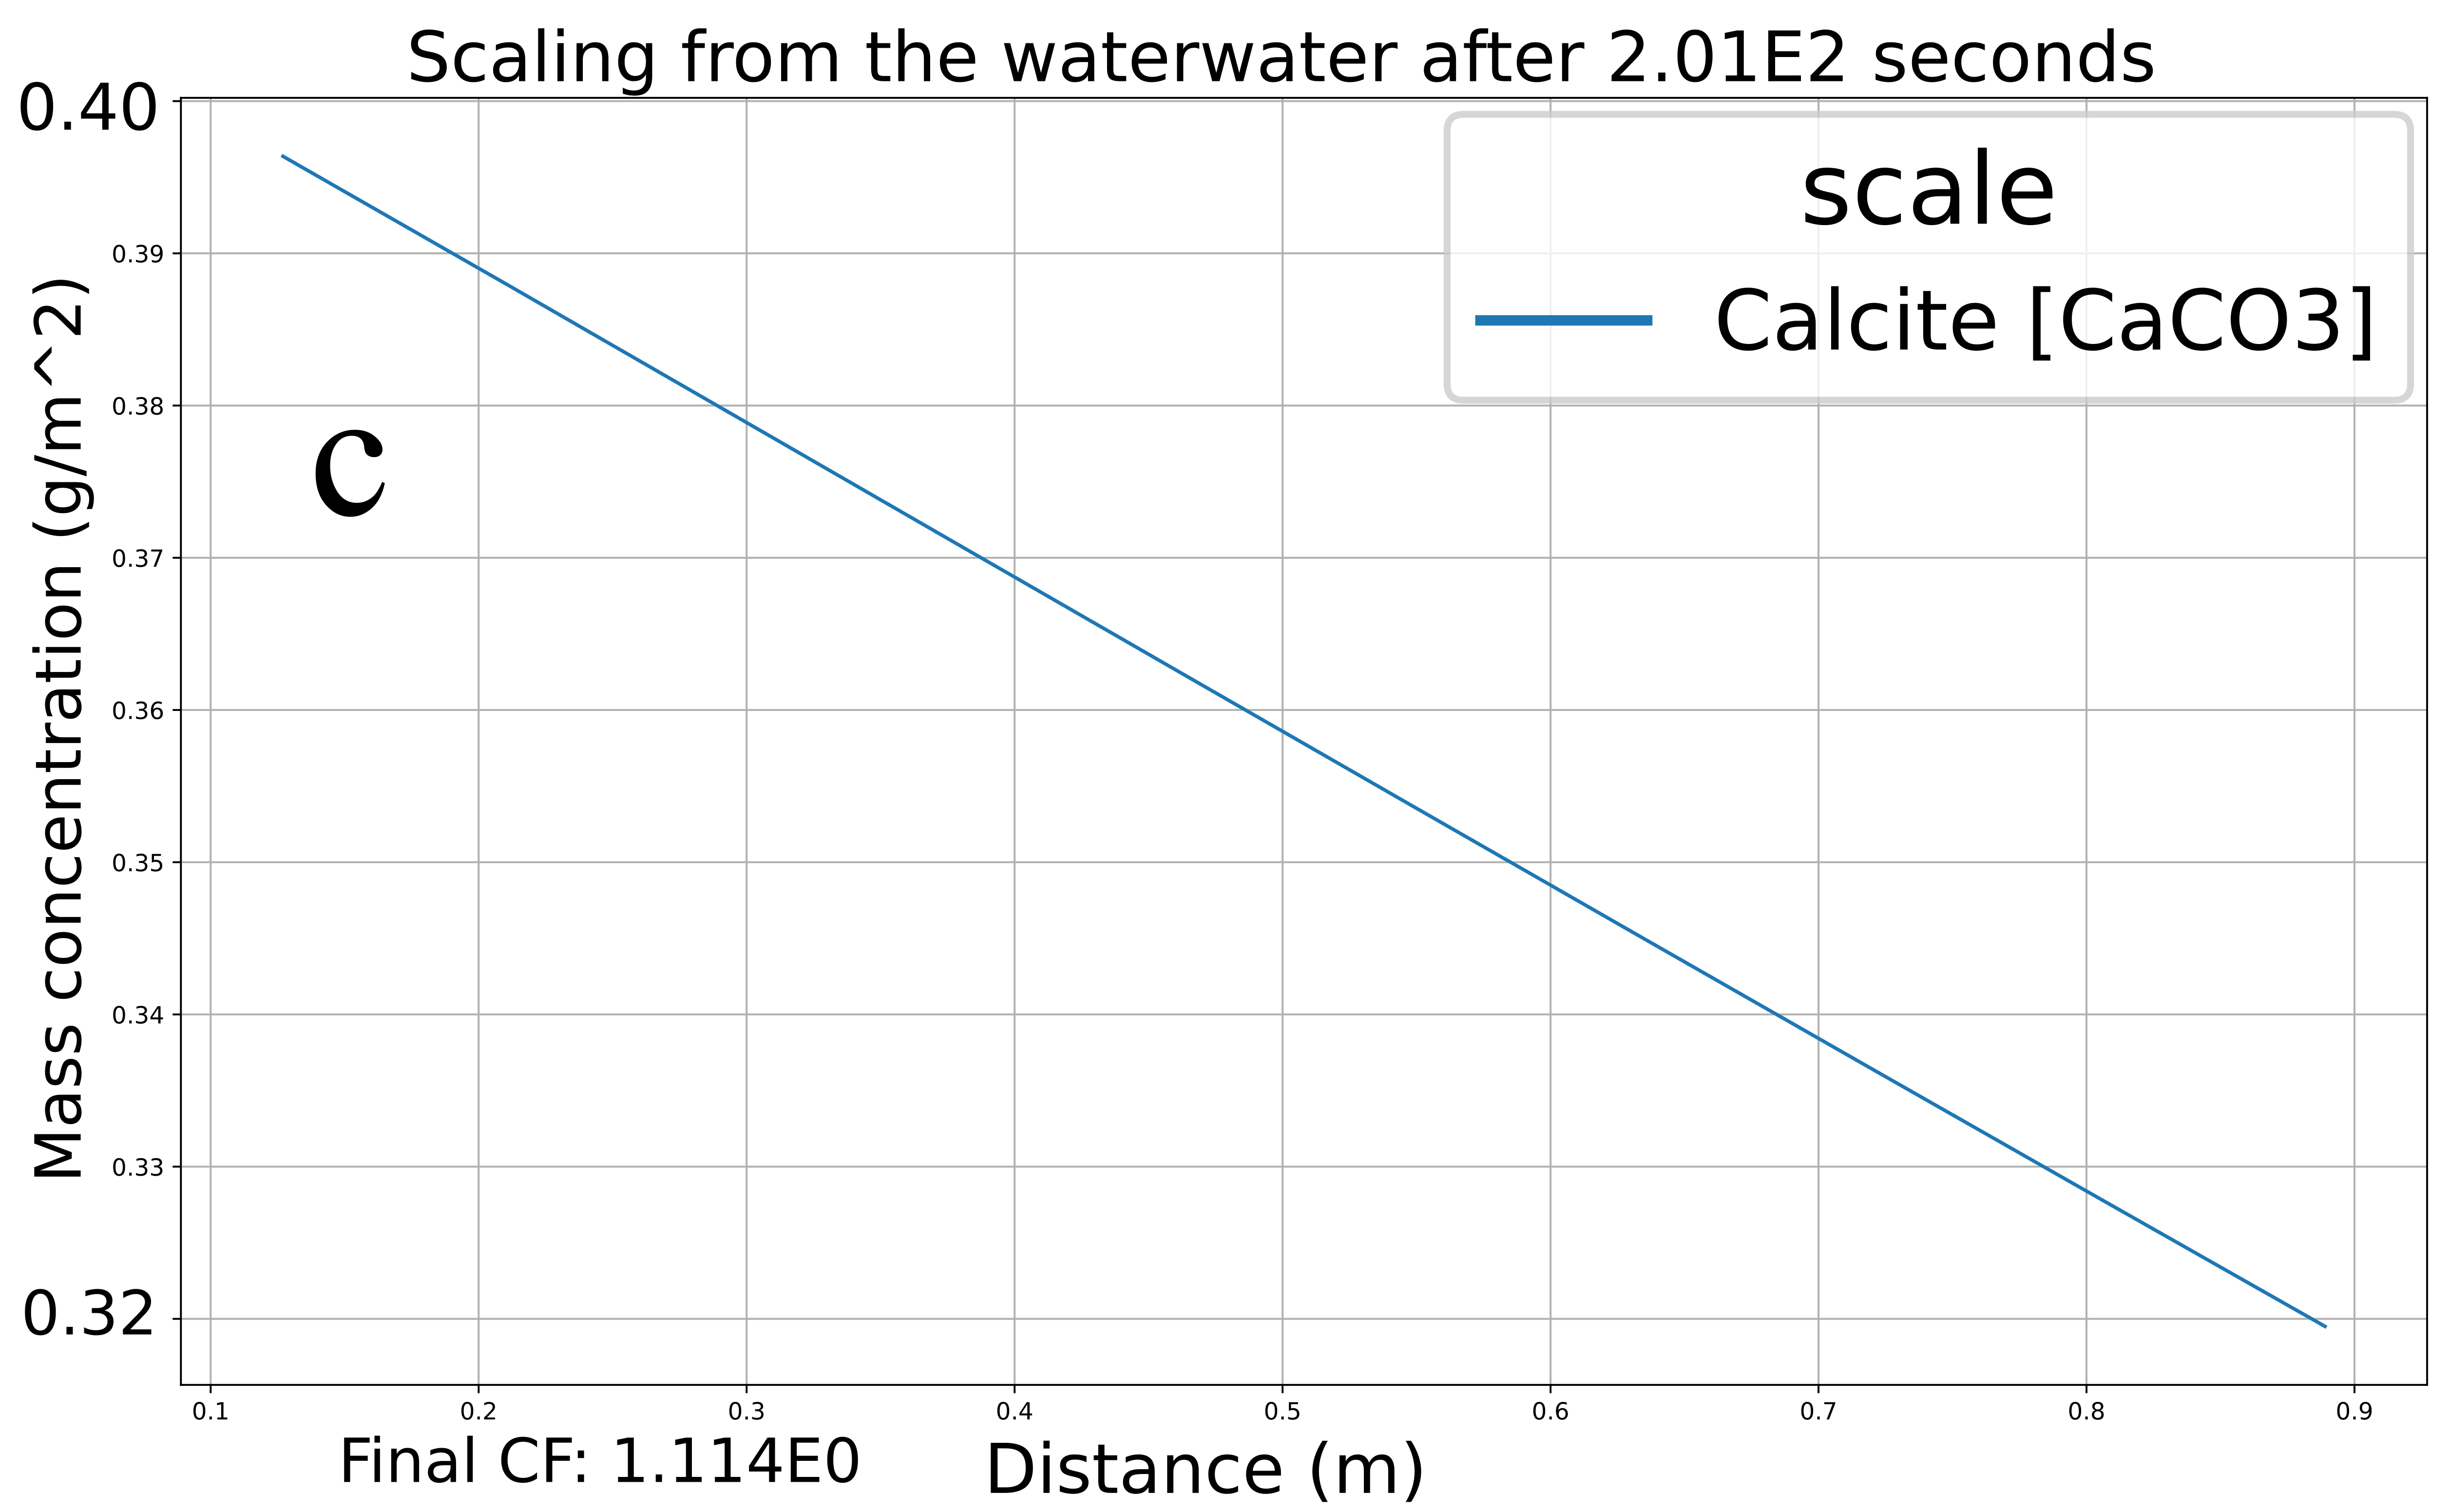
\includegraphics[width=0.49\linewidth]{images/ROSSpy/case_studies/Lee_pitzer.png} \\
    \end{tabular}
    \caption{
        The qualitative validation of scaling for a) multiple minerals from the Karabelas et al., 2020 study; b) Gypsum in the Karabelas et al., 2014 study; and c) Calcite in the Lee et al. study. 
    }
    \label{qualitative_scaling}
\end{figure}


\section{Sensitivity analyses}
A few sensitivity analyses were conducted with major variables in the following subsections. Additional sensitivity analyses of lesser parameters are presented in the Supporting Information.

\subsection{Database section}
The PHREEQC databases crucially 1) determines the set of minerals that can be simulated; 2) contains all of the kinetic, thermodynamic, and stoichiometric information of each mineral; and 3) employs a chemical activity model: e.g. Pitzer, Debye-H\"uckel, and Davies in Section 7 of the Supporting Information. The Pitzer model \cite{Pitzer1973ThermodynamicsEquations,Pitzer1974ThermodynamicsElectrolytes}, which is implemented in the pitzer PHREEQC database, is touted as being supremely accurate in the concentration range of desalination \cite{VandeLisdonk2001PredictionSystems,Sheikholeslami2004AssessmentUnits,Mohammad2007PredictionMembranes}; however, the narrow breadth of accepted ions and minerals may justify using other databases, such as wateq4, for complex or uncommon feed sources. Each of the 13 databases were simulated in desalinating the Red Sea, where the $Amm$, $Core10$, $LLNL$, and $Minteq.v4$ databases failed to numerically converge while the scaling predictions from the other $\frac{9}{13}$ databases are summarized in Figure \ref{database_selection}. The database selection evidently alters scaling predictions; thus, the database must be carefully selected for a given system after reviewing the PHREEQC User Manual or inquirying to the PHREEQC user forum \url{PHREEQCusers.org}.

\begin{figure}
    \centering
    \begin{tabular}{c|c}
        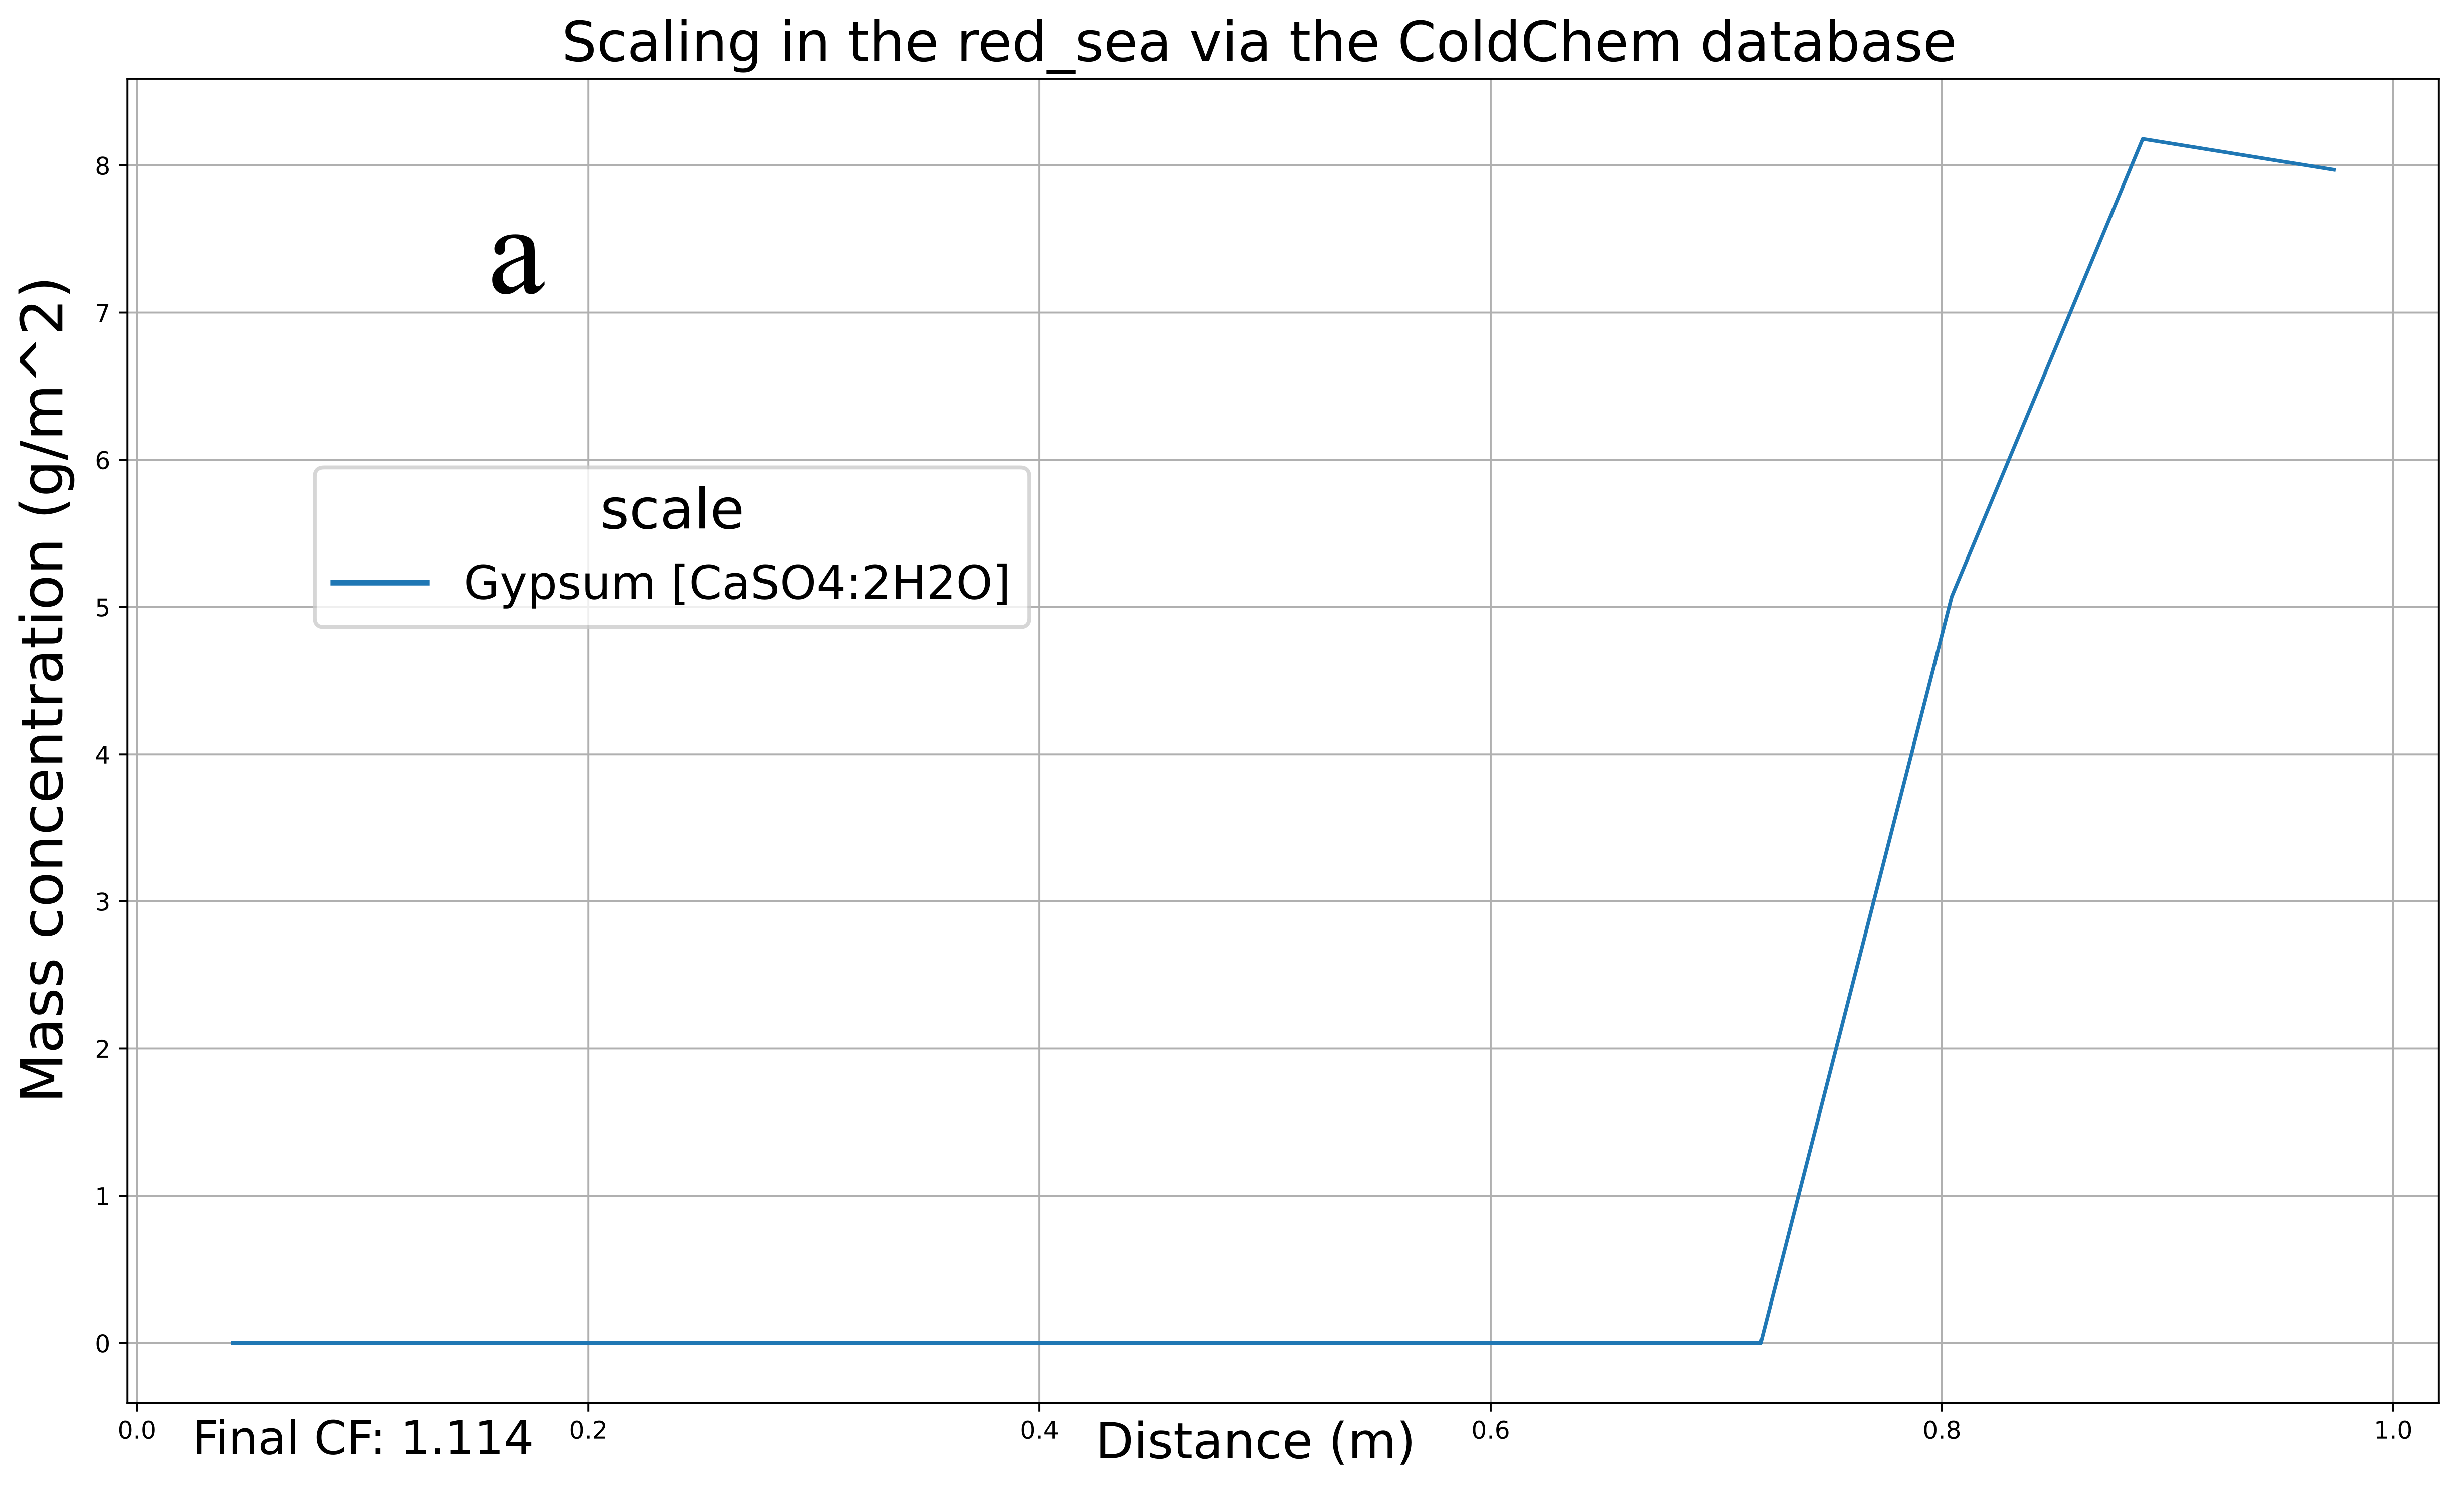
\includegraphics[width=0.49\textwidth]{images/ROSSpy/sensitivity_analyses/databases/ColdChem.png} 
        & 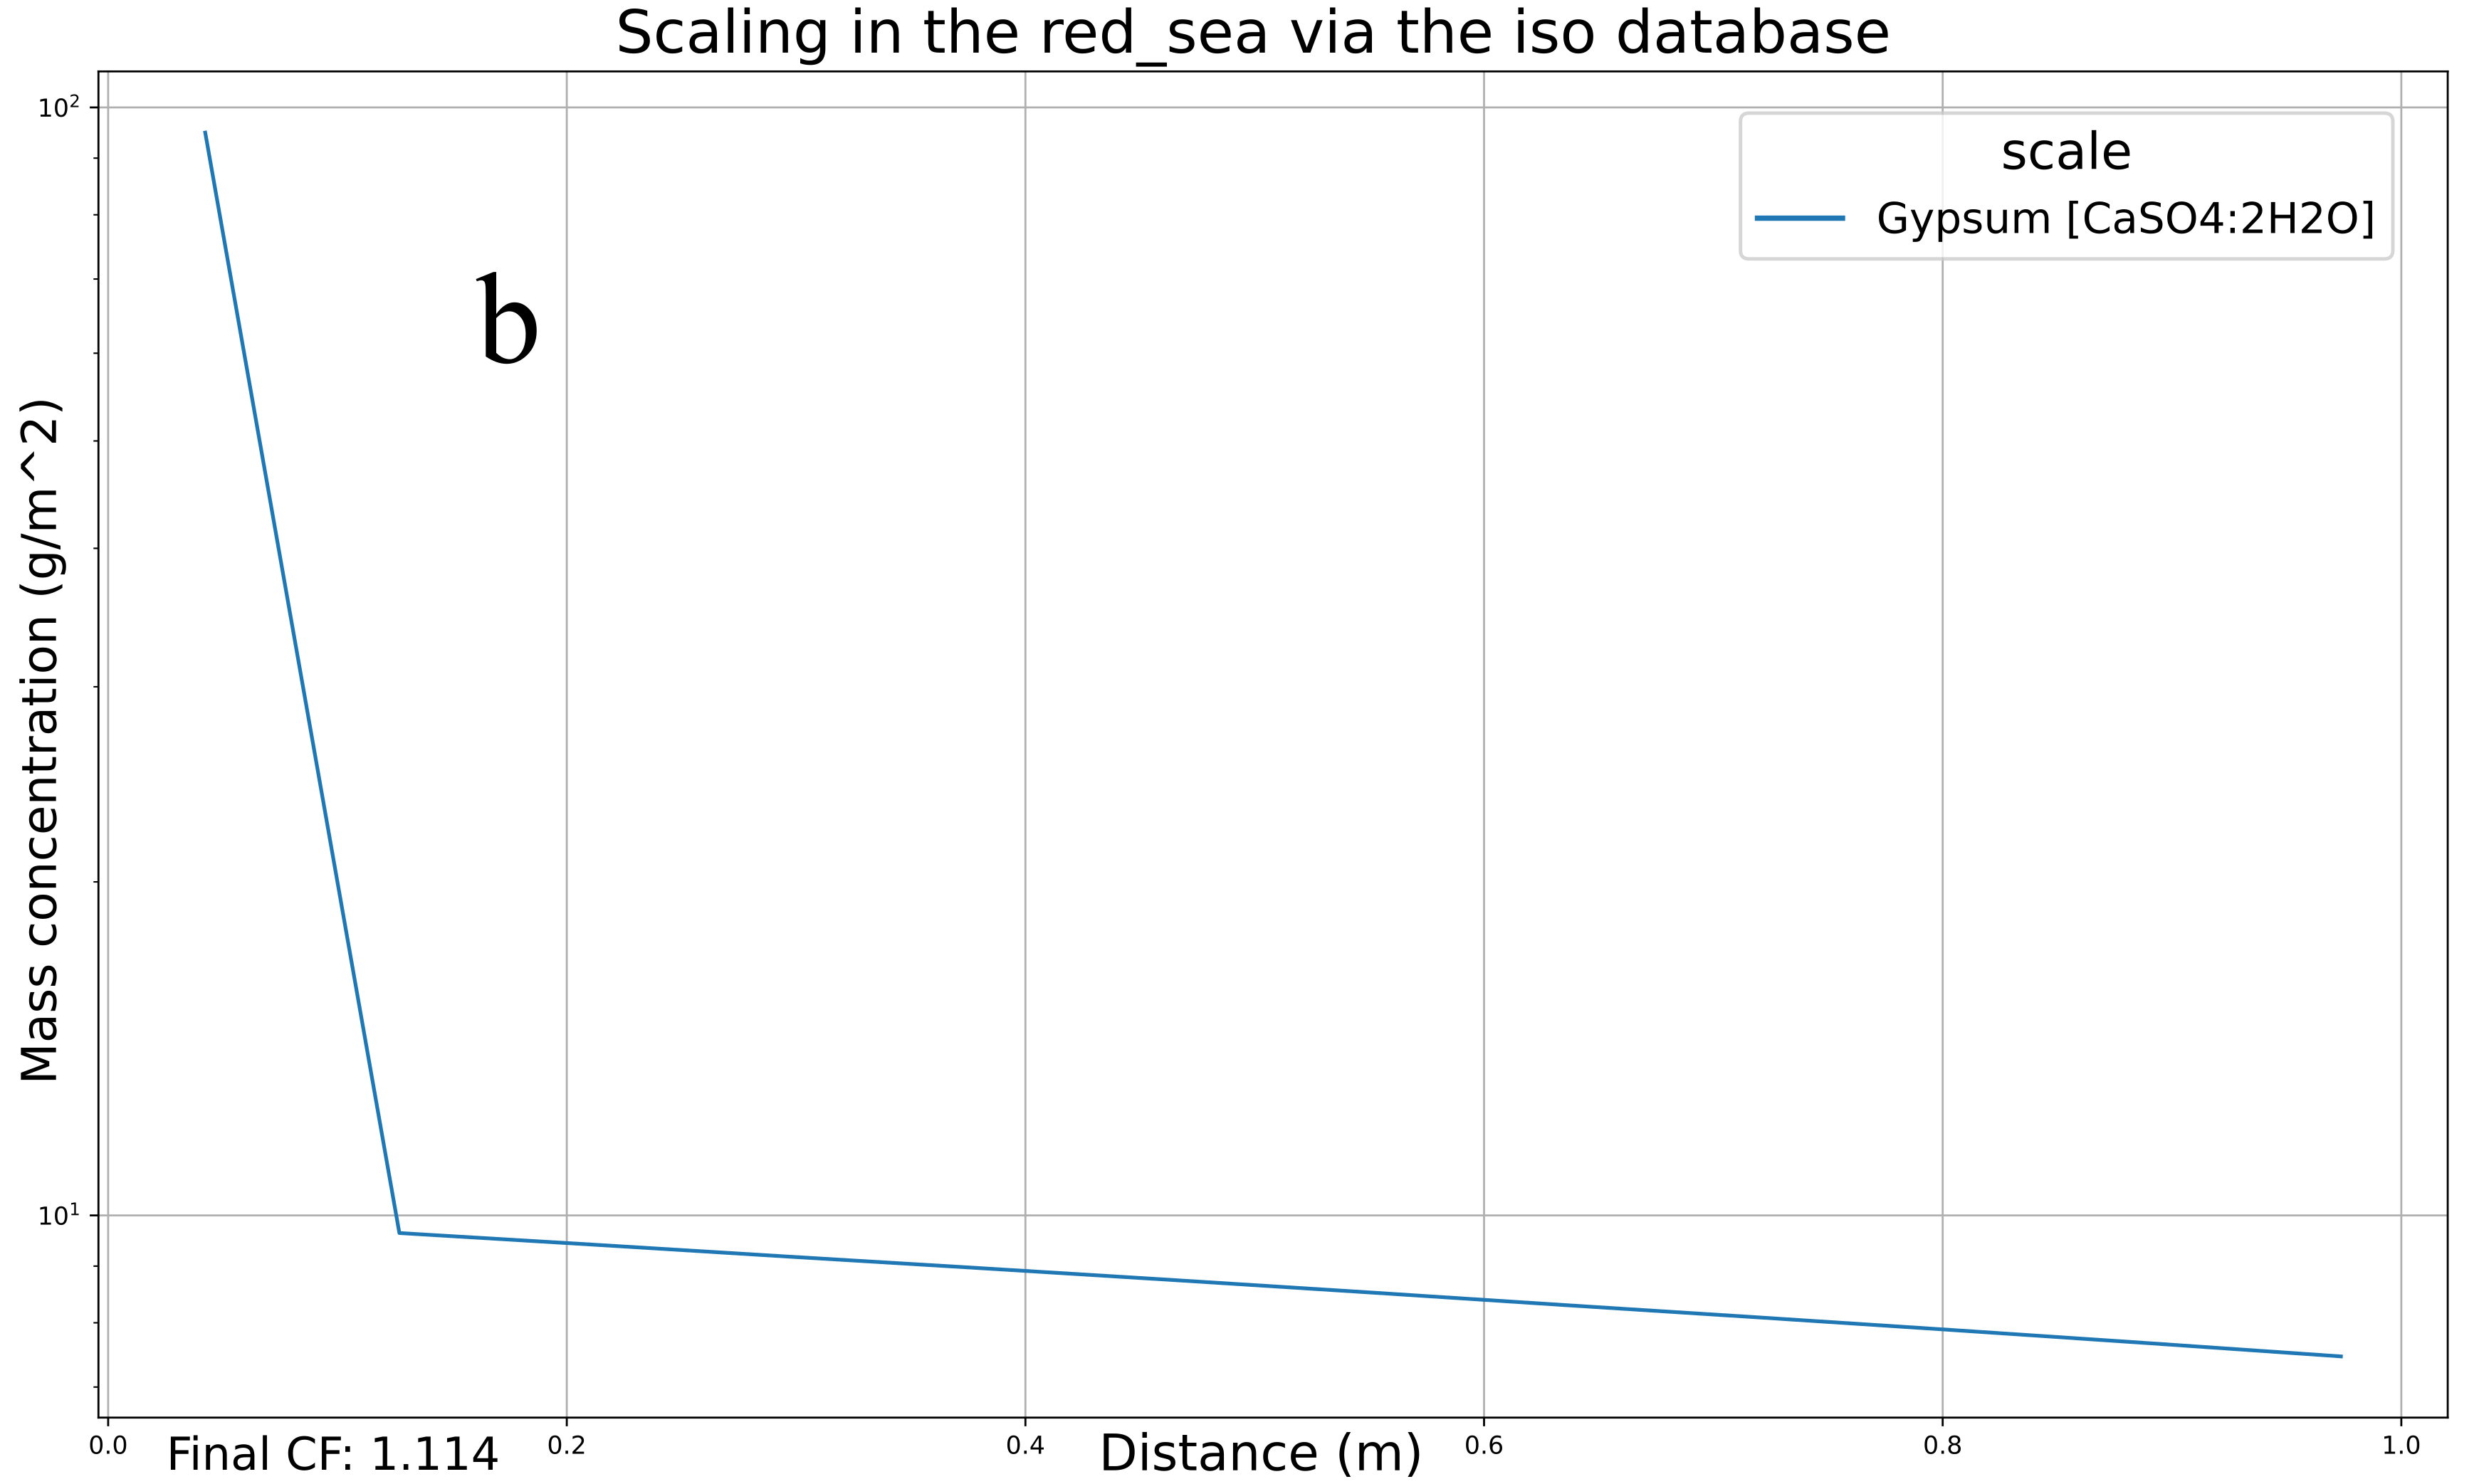
\includegraphics[width=0.49\textwidth]{images/ROSSpy/sensitivity_analyses/databases/Iso.png} \\ \midrule 
        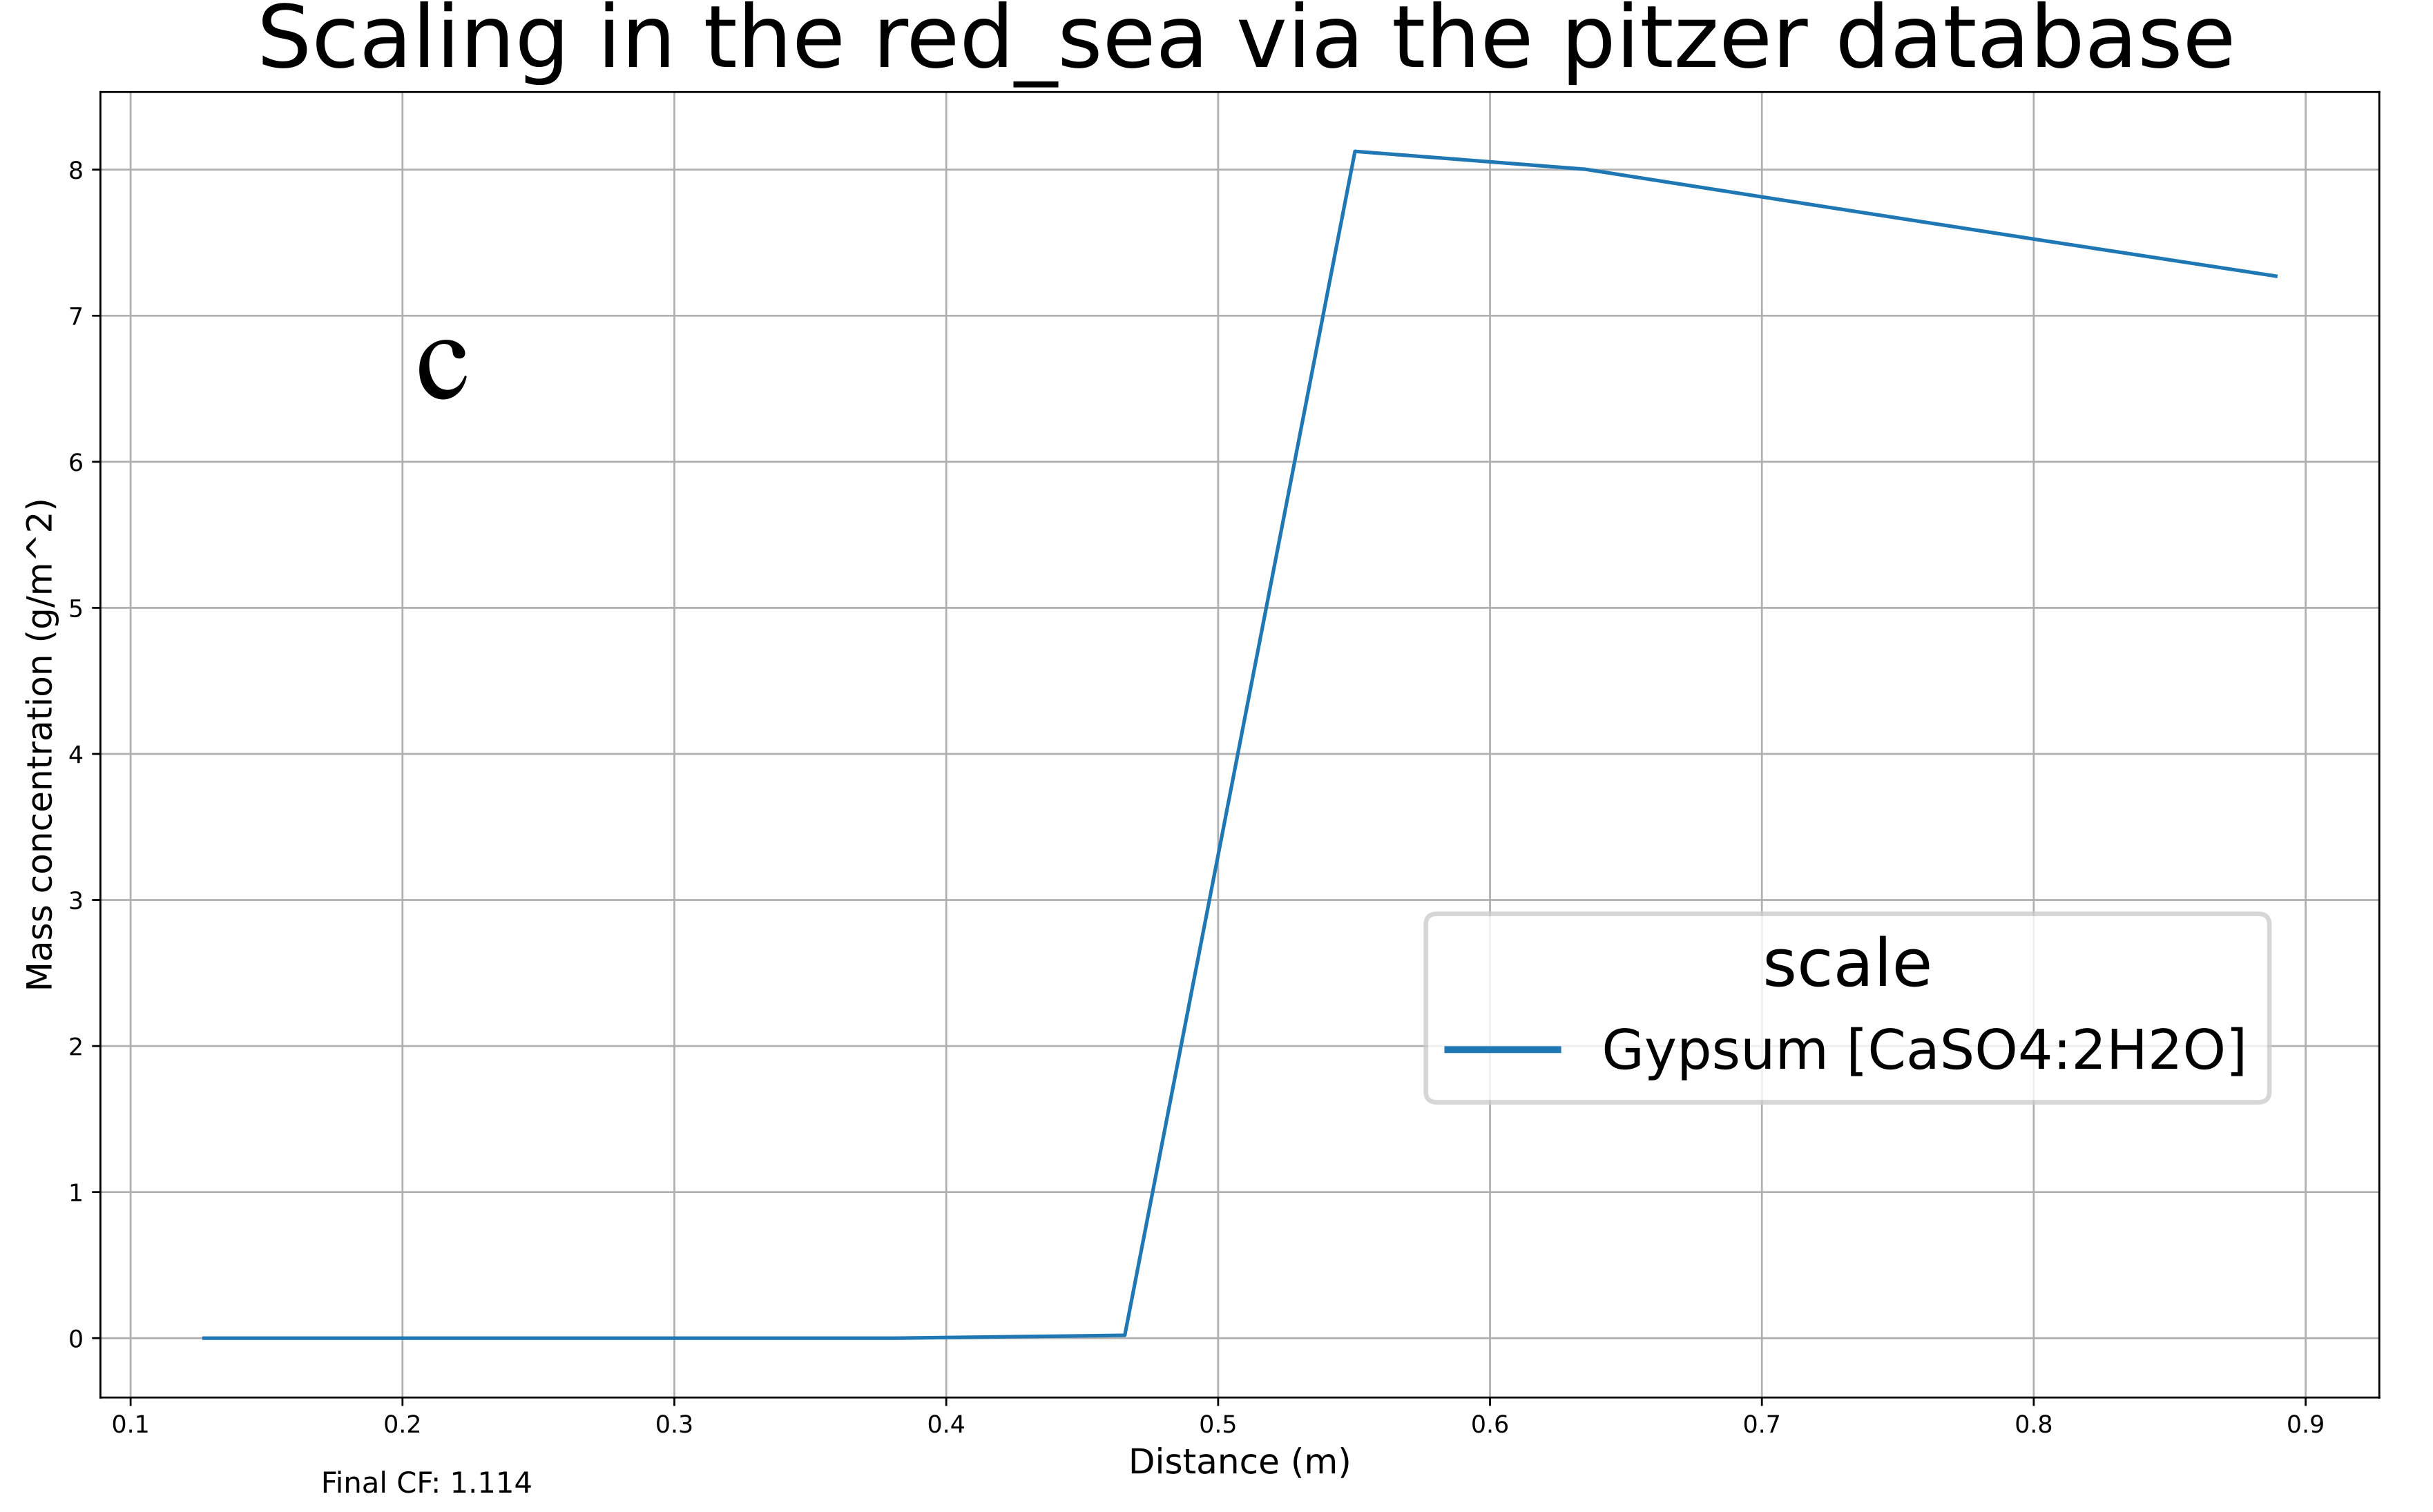
\includegraphics[width=0.49\textwidth]{images/ROSSpy/sensitivity_analyses/databases/Pitzer.png} 
        & 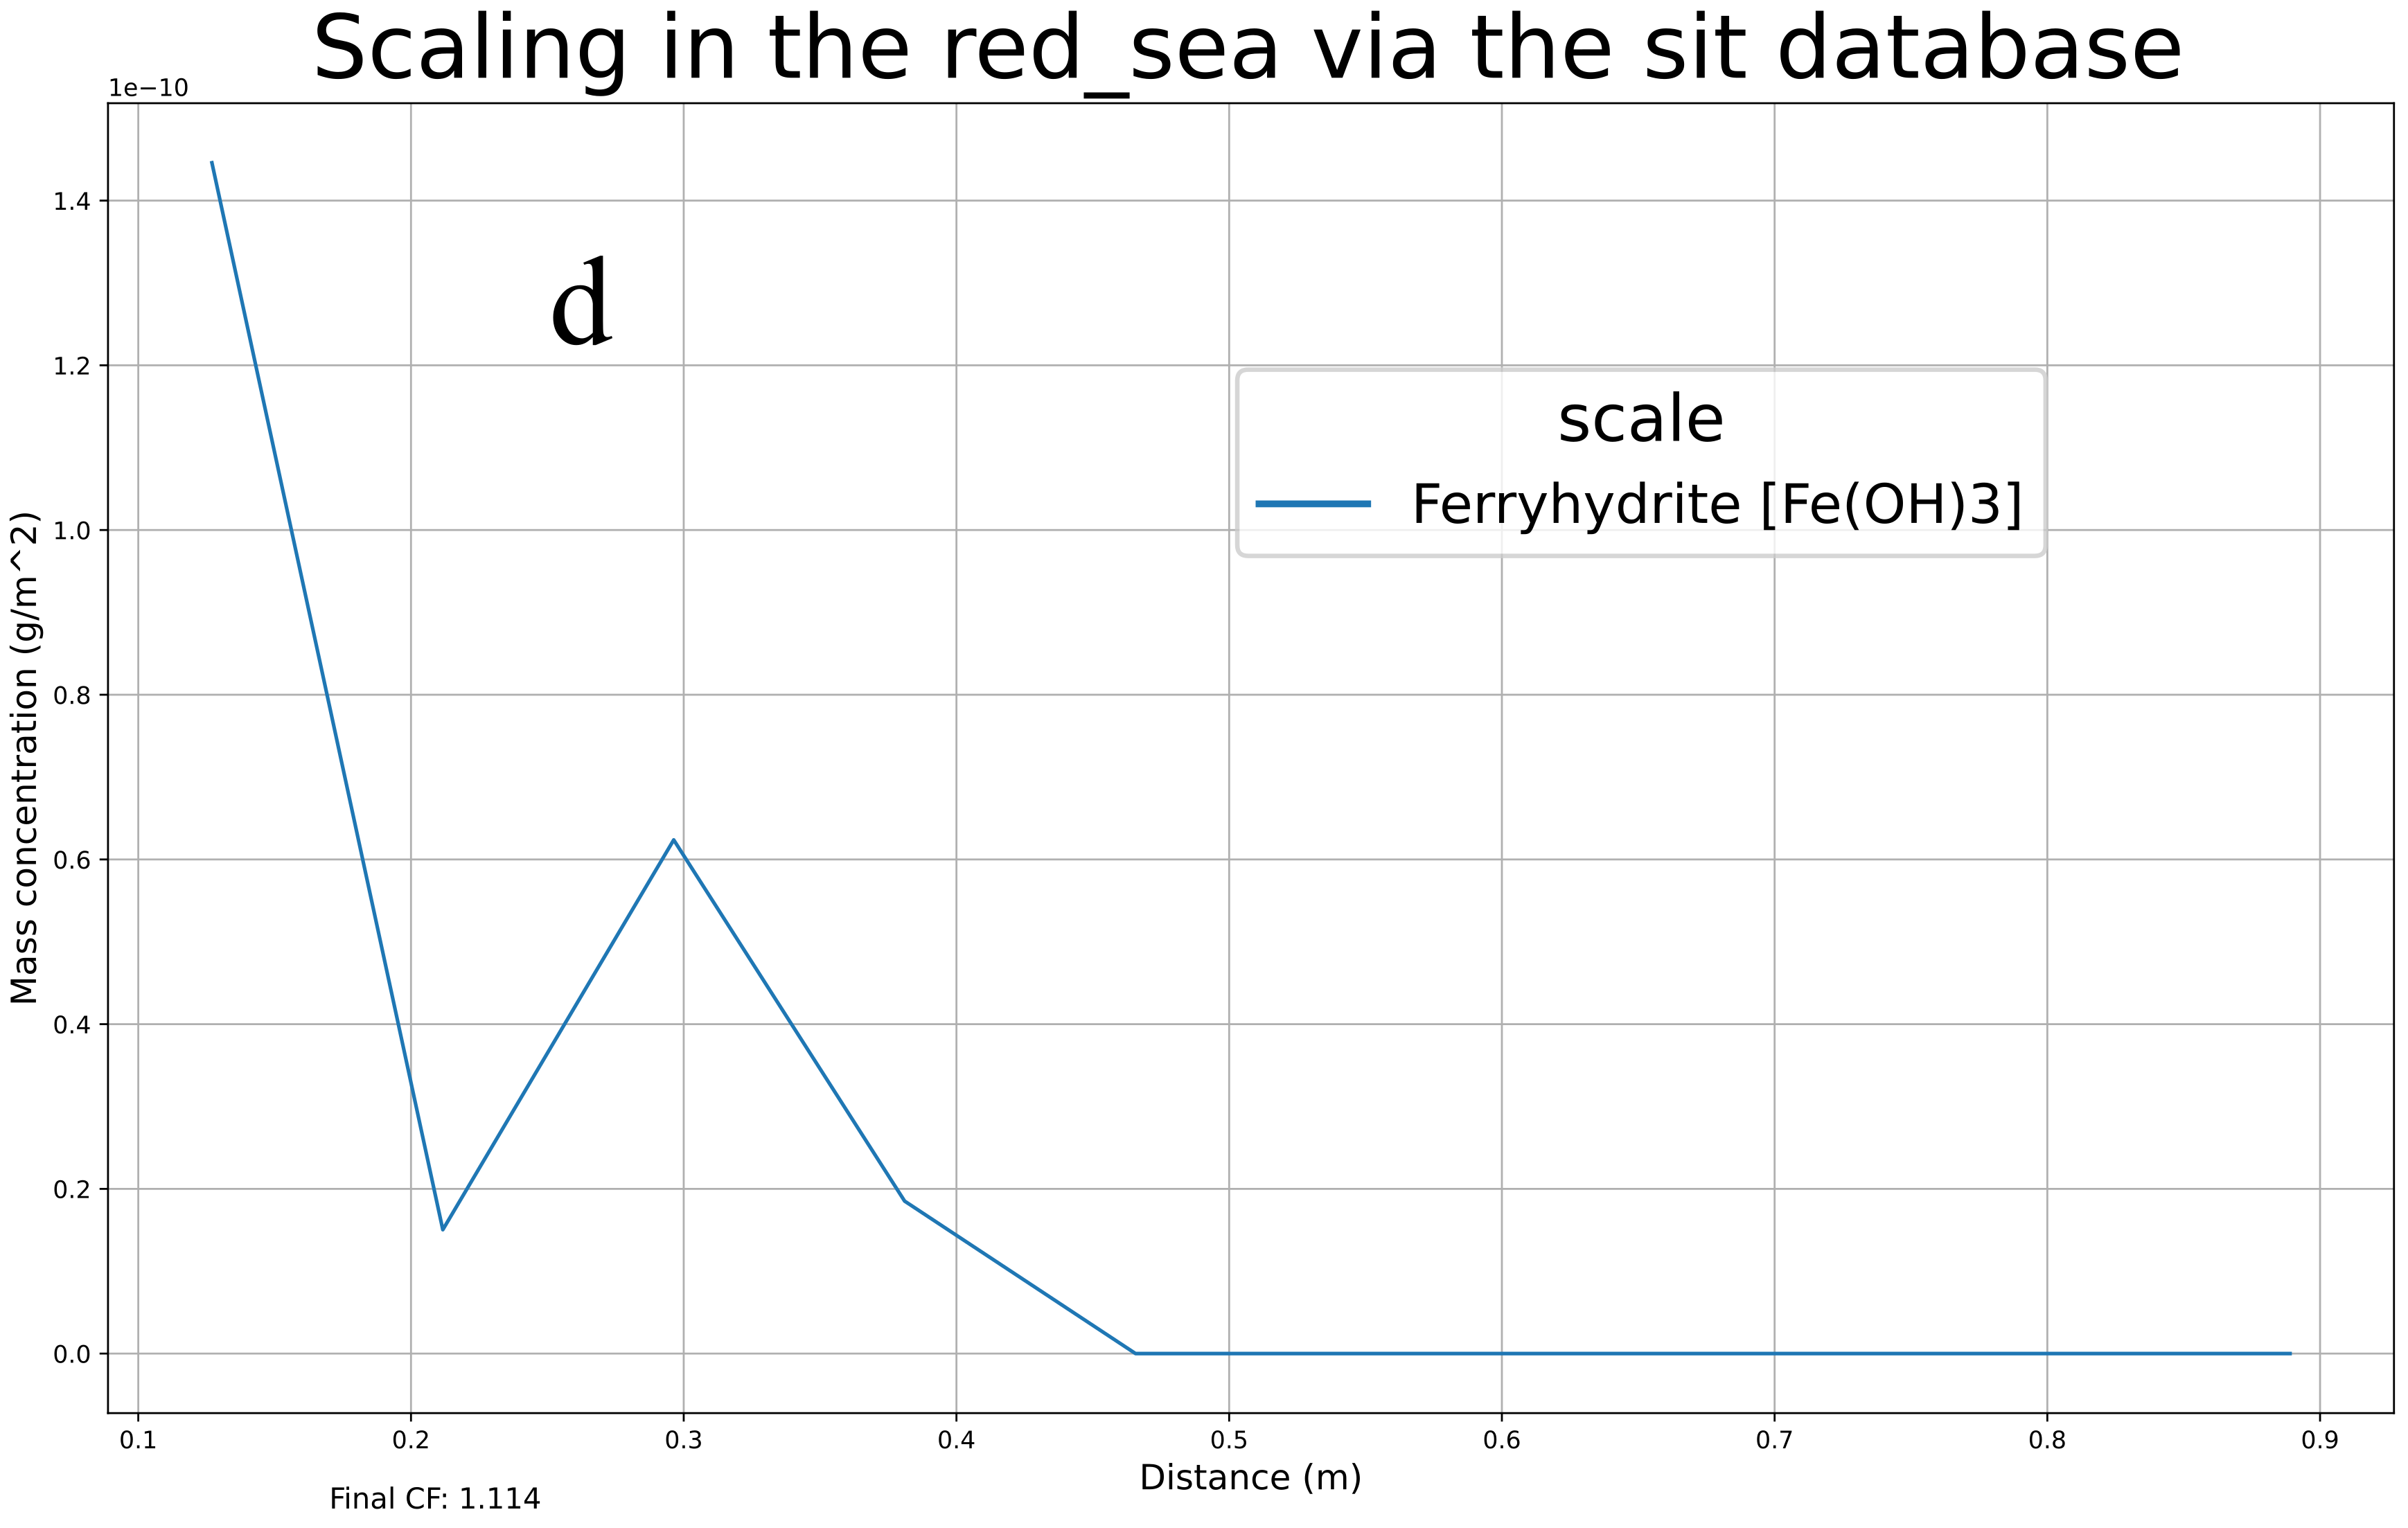
\includegraphics[width=0.49\textwidth]{images/ROSSpy/sensitivity_analyses/databases/Sit.png} 
        \\ \bottomrule
    \end{tabular}
    \caption{
        Scaling predictions from the a) ColdChem, b) Iso, c) Pitzer, and d) Sit databases, with otherwise identical simulation parameters. These subfigures represent the spectrum of similar yet distinct predictions of scaling during the database sensitivity analysis, and exemplify that the PHREEQC database should be deliberately selected after reviewing the PHREEQC documentation to discern which database is most appropriate for the feed geochemistry.
    }
    \label{database_selection}
\end{figure}

\subsection{Feed geochemistry}
The default feed waters were constructed from experimental geochemical literature into parameter files that are provided with ROSSpy. Users of ROSSpy are encouraged to simulate their own feed water while emulating the syntax of the default parameter files. We propose experimental data of numerous other water sources in Section 5 of the Supporting Information that can predicate feed water files; although, direct measurement of the simulated feed water is preferable to avoid significant influences of anthropogenic pollution \cite{Chen2008SourcesSea} and seasonality \cite{Sarthou2001SeasonalSea} in reported measurements. Thee default water sources, which include both natural seas and produced waters from oil wells, were contrasted in Figure \ref{feed_sources}, where the scaling and brine predictions differed significantly amongst these feed water sources. 

\begin{figure}
    \centering
    \begin{tabular}{c|c}
        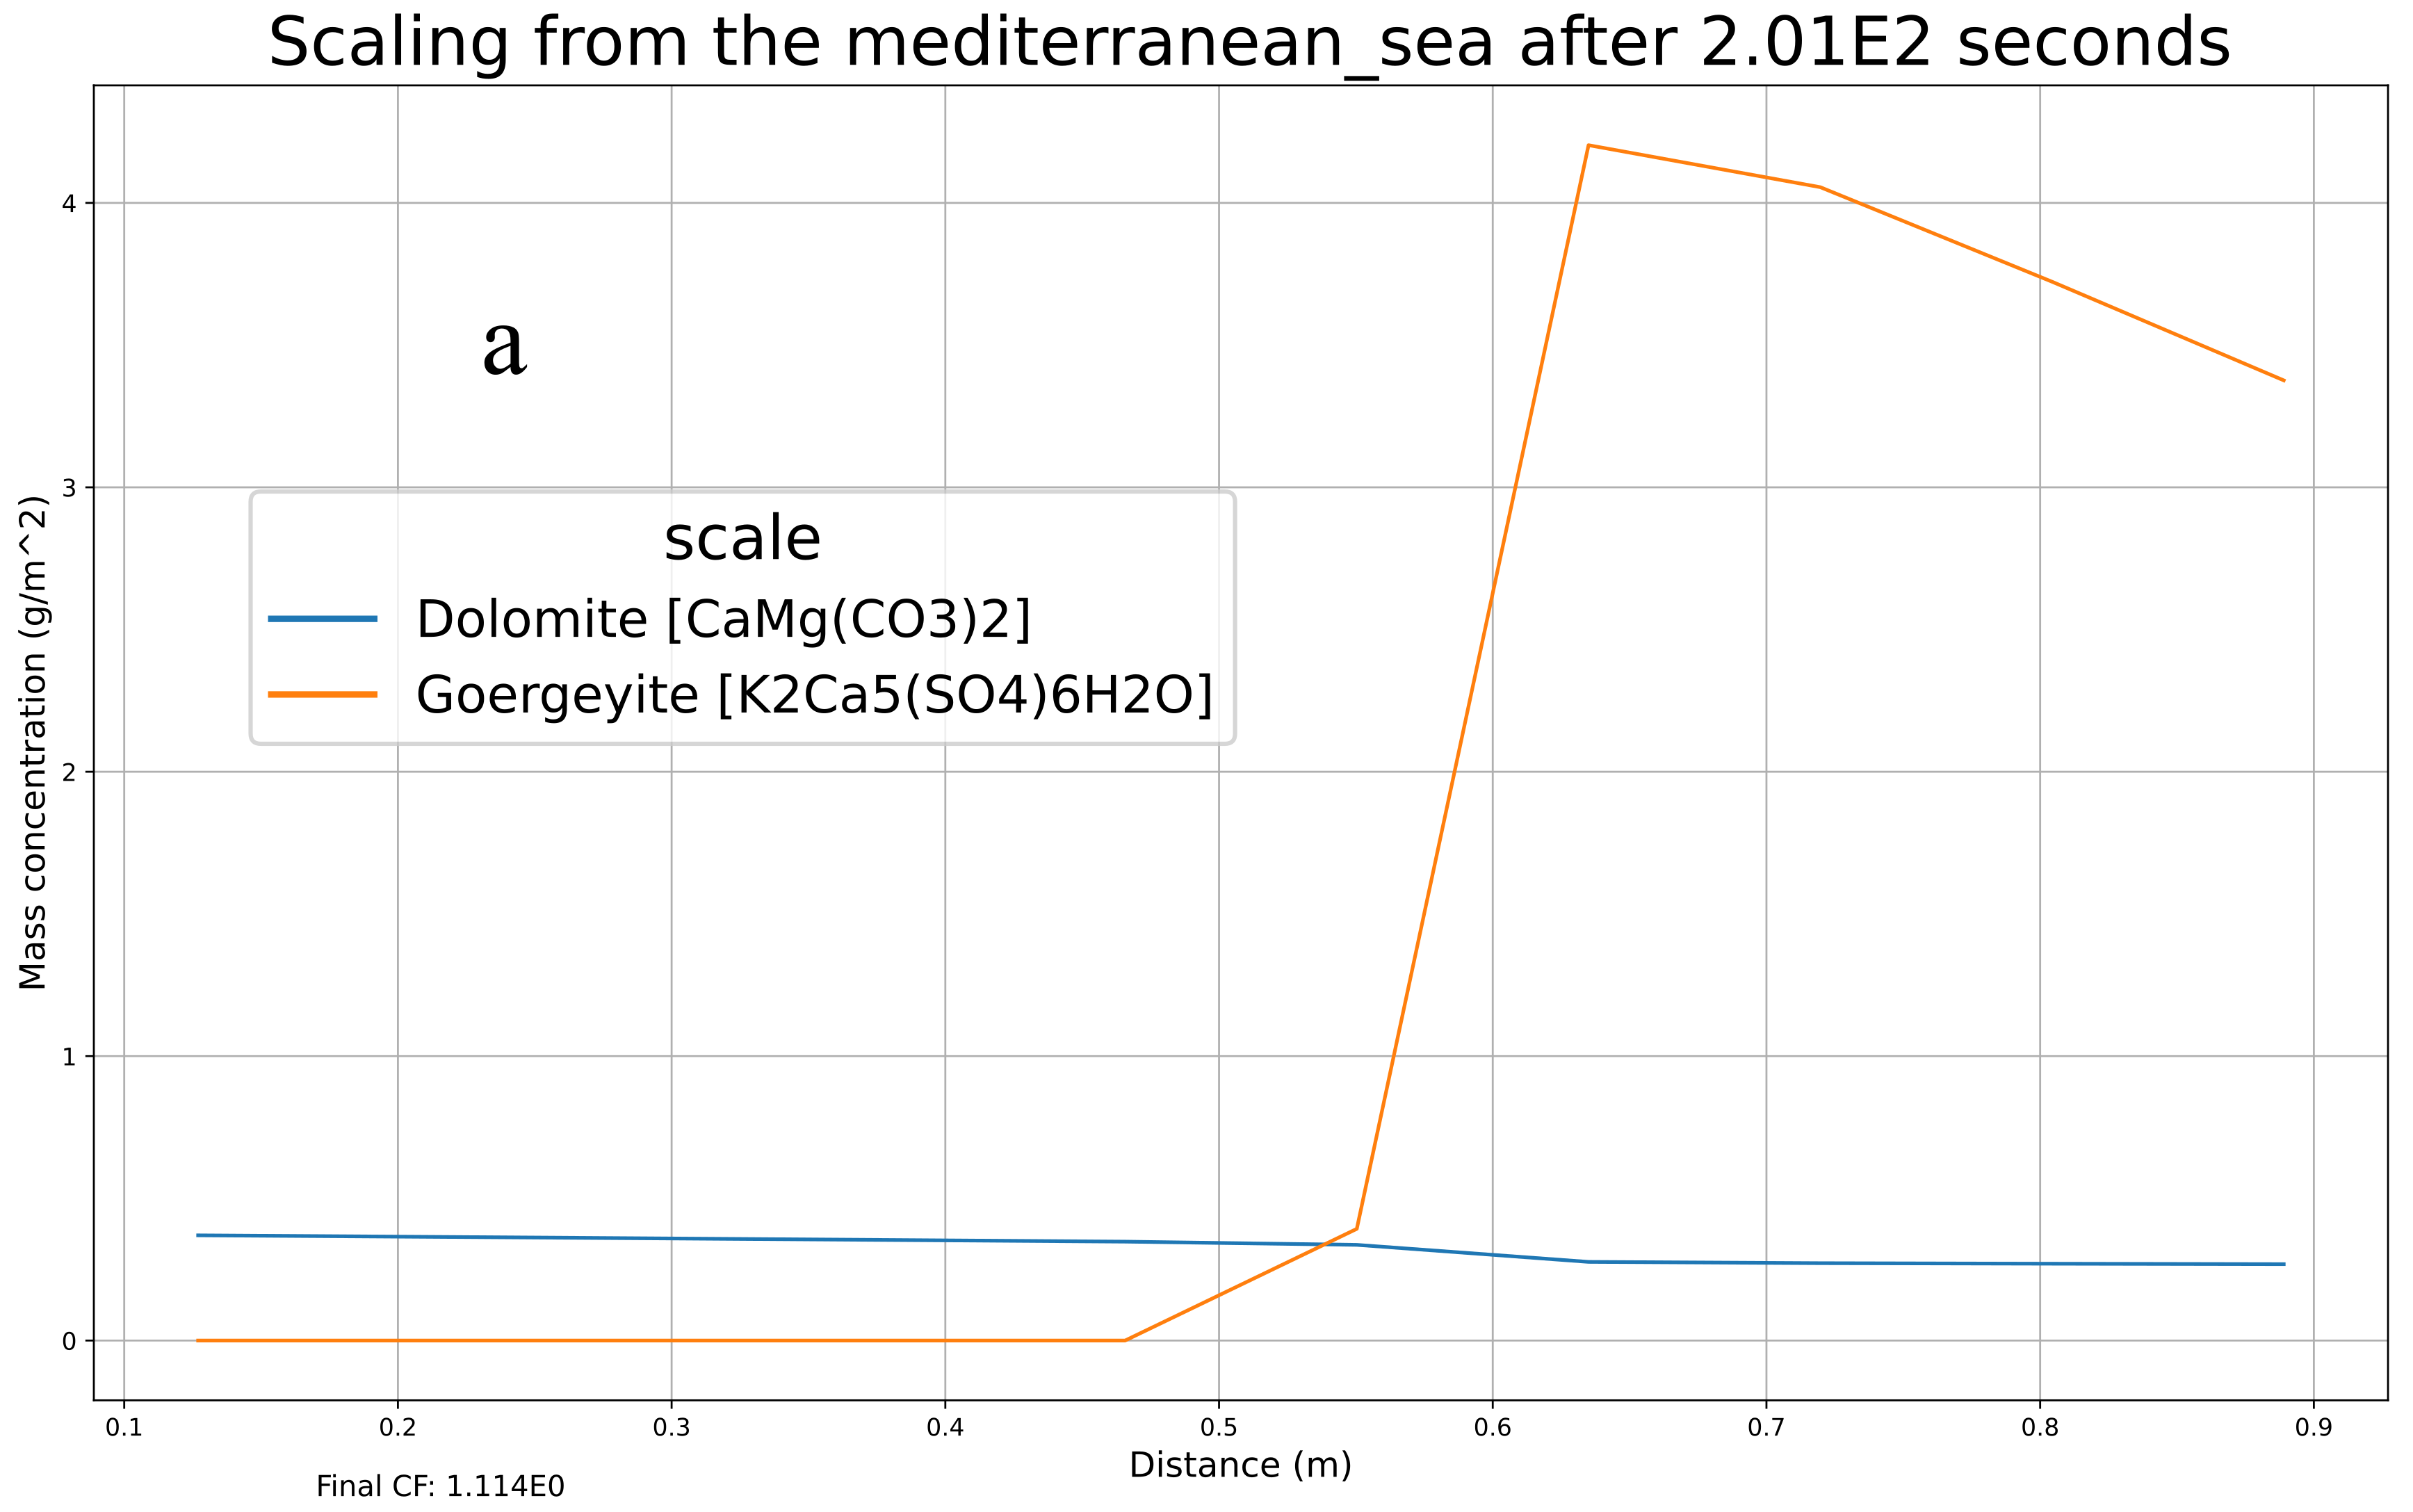
\includegraphics[width=0.49\textwidth]{images/ROSSpy/sensitivity_analyses/feed_source/Mediterranean.png} &
        \includegraphics[width=0.49\textwidth]{images/ROSSpy/sensitivity_analyses/feed_source/Palo_Duro_basin.png} \\ \midrule
        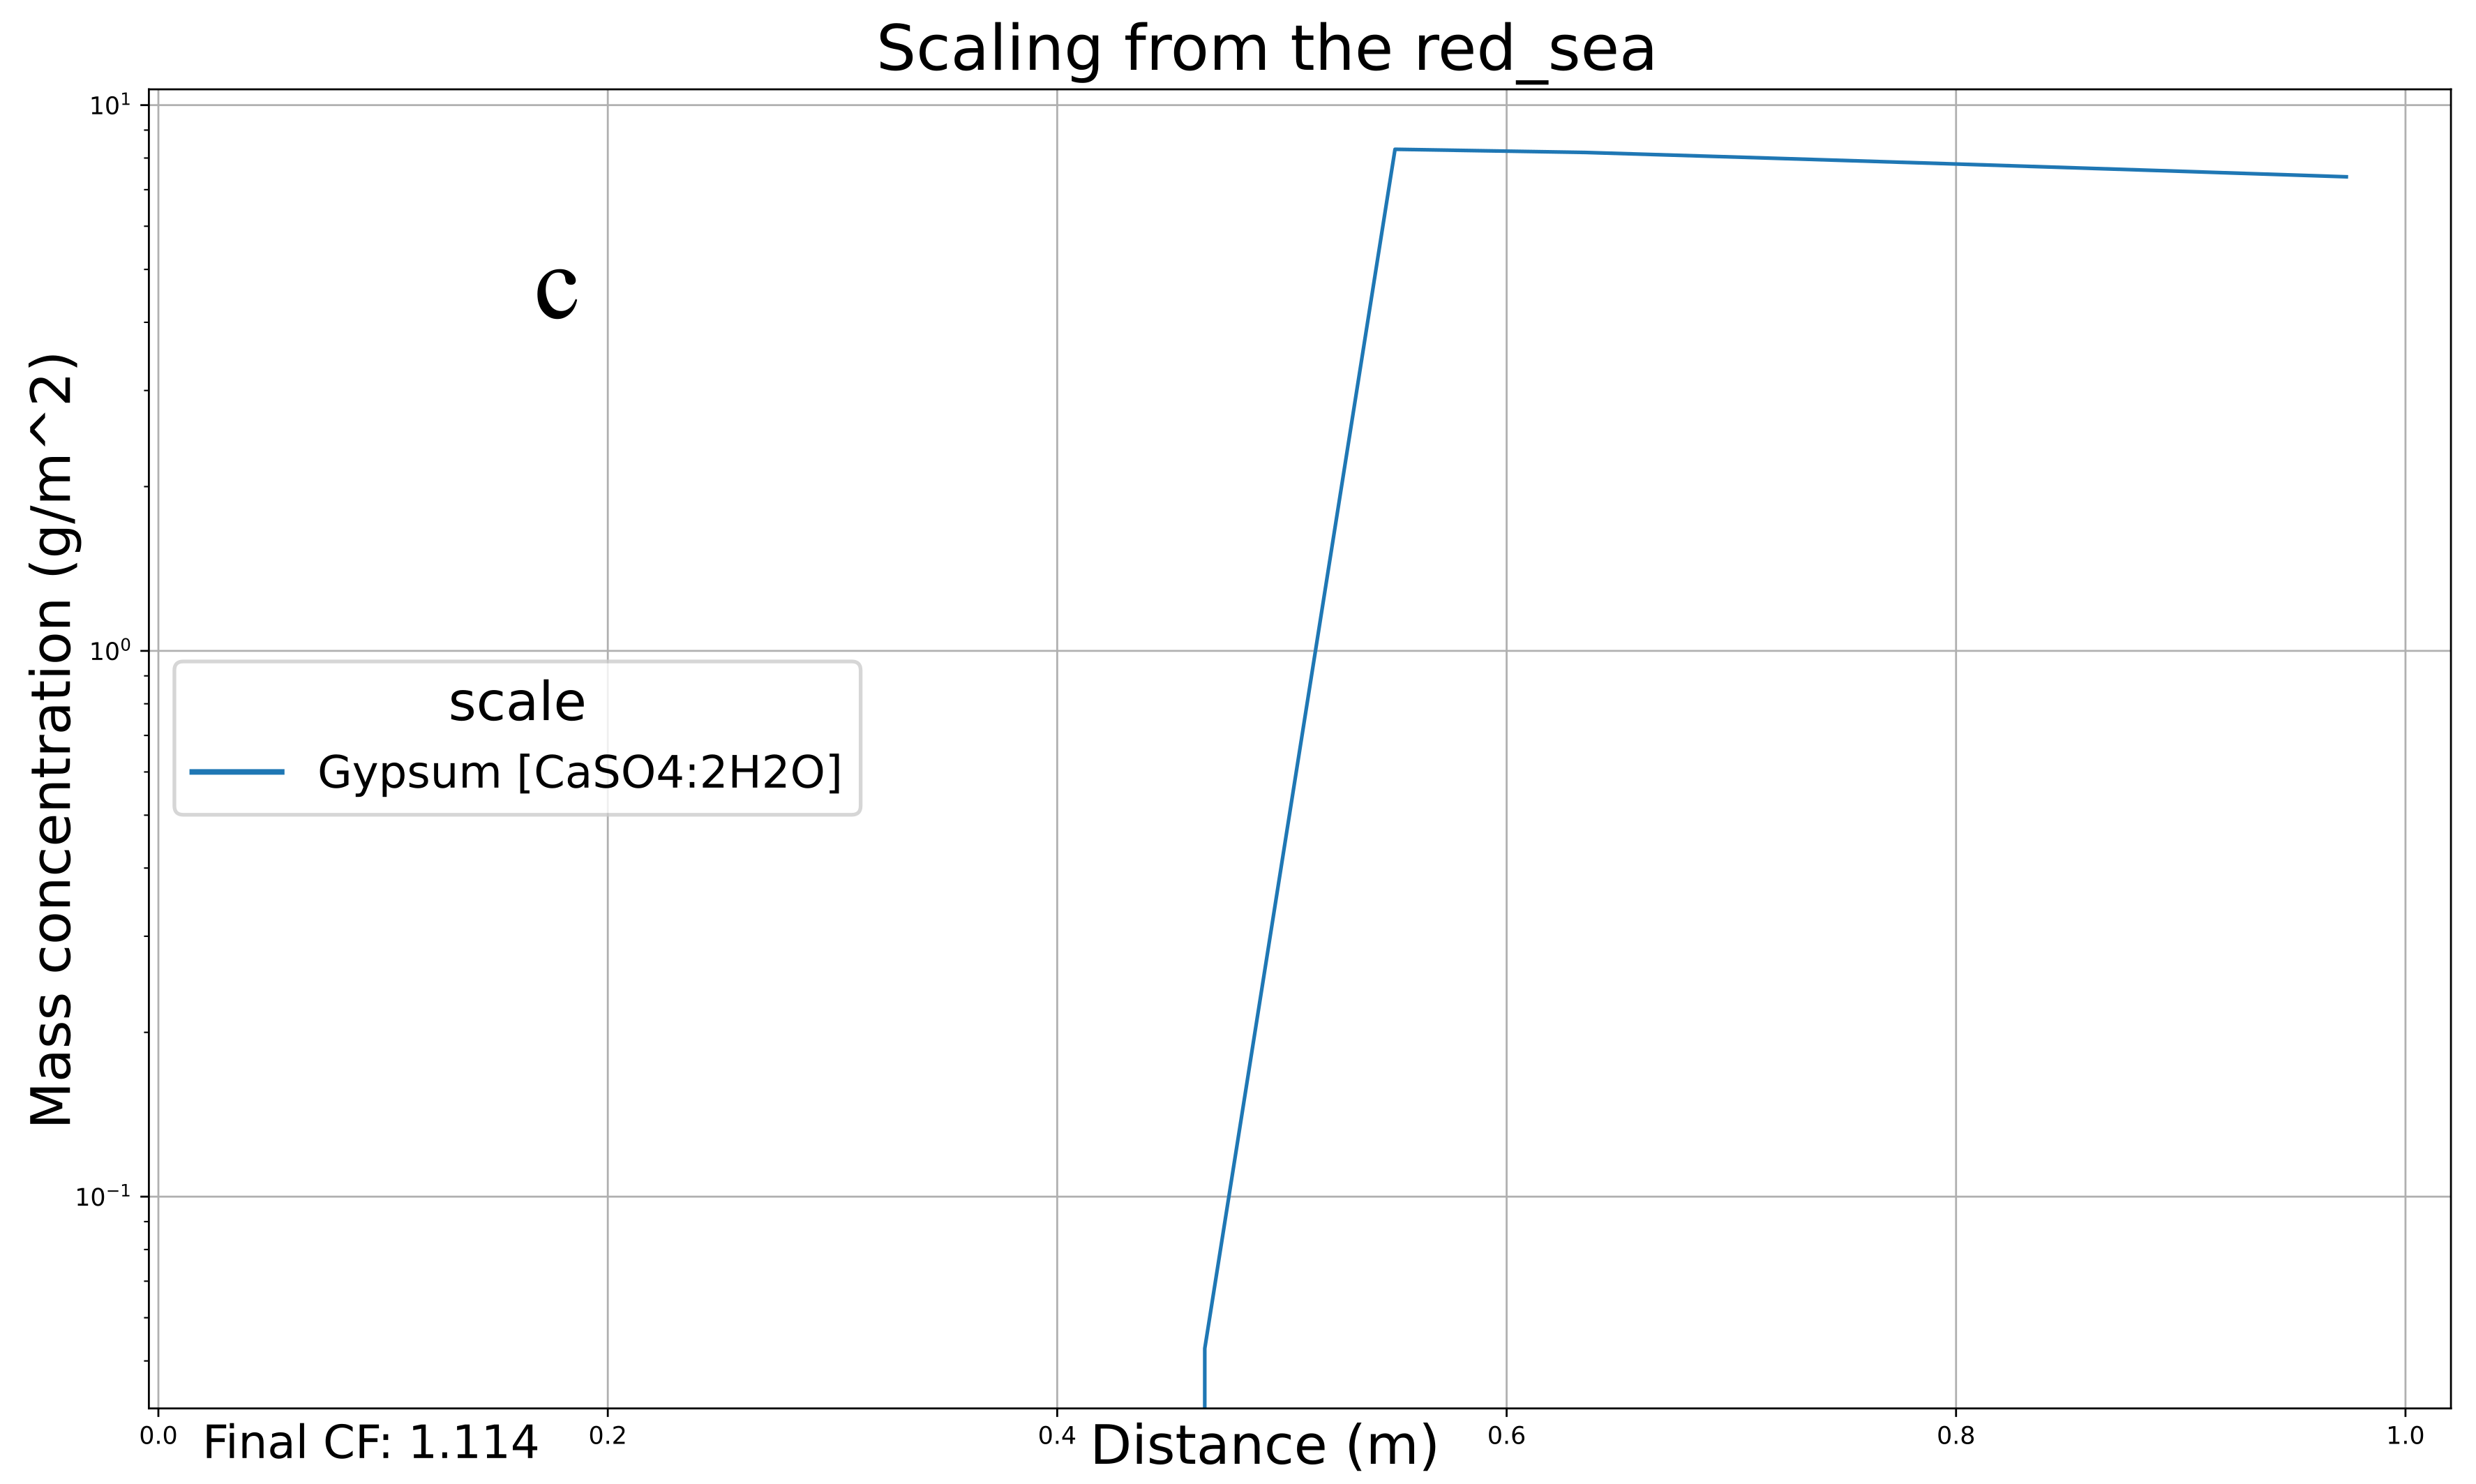
\includegraphics[width=0.49\textwidth]{images/ROSSpy/sensitivity_analyses/feed_source/Red_Sea.png} & 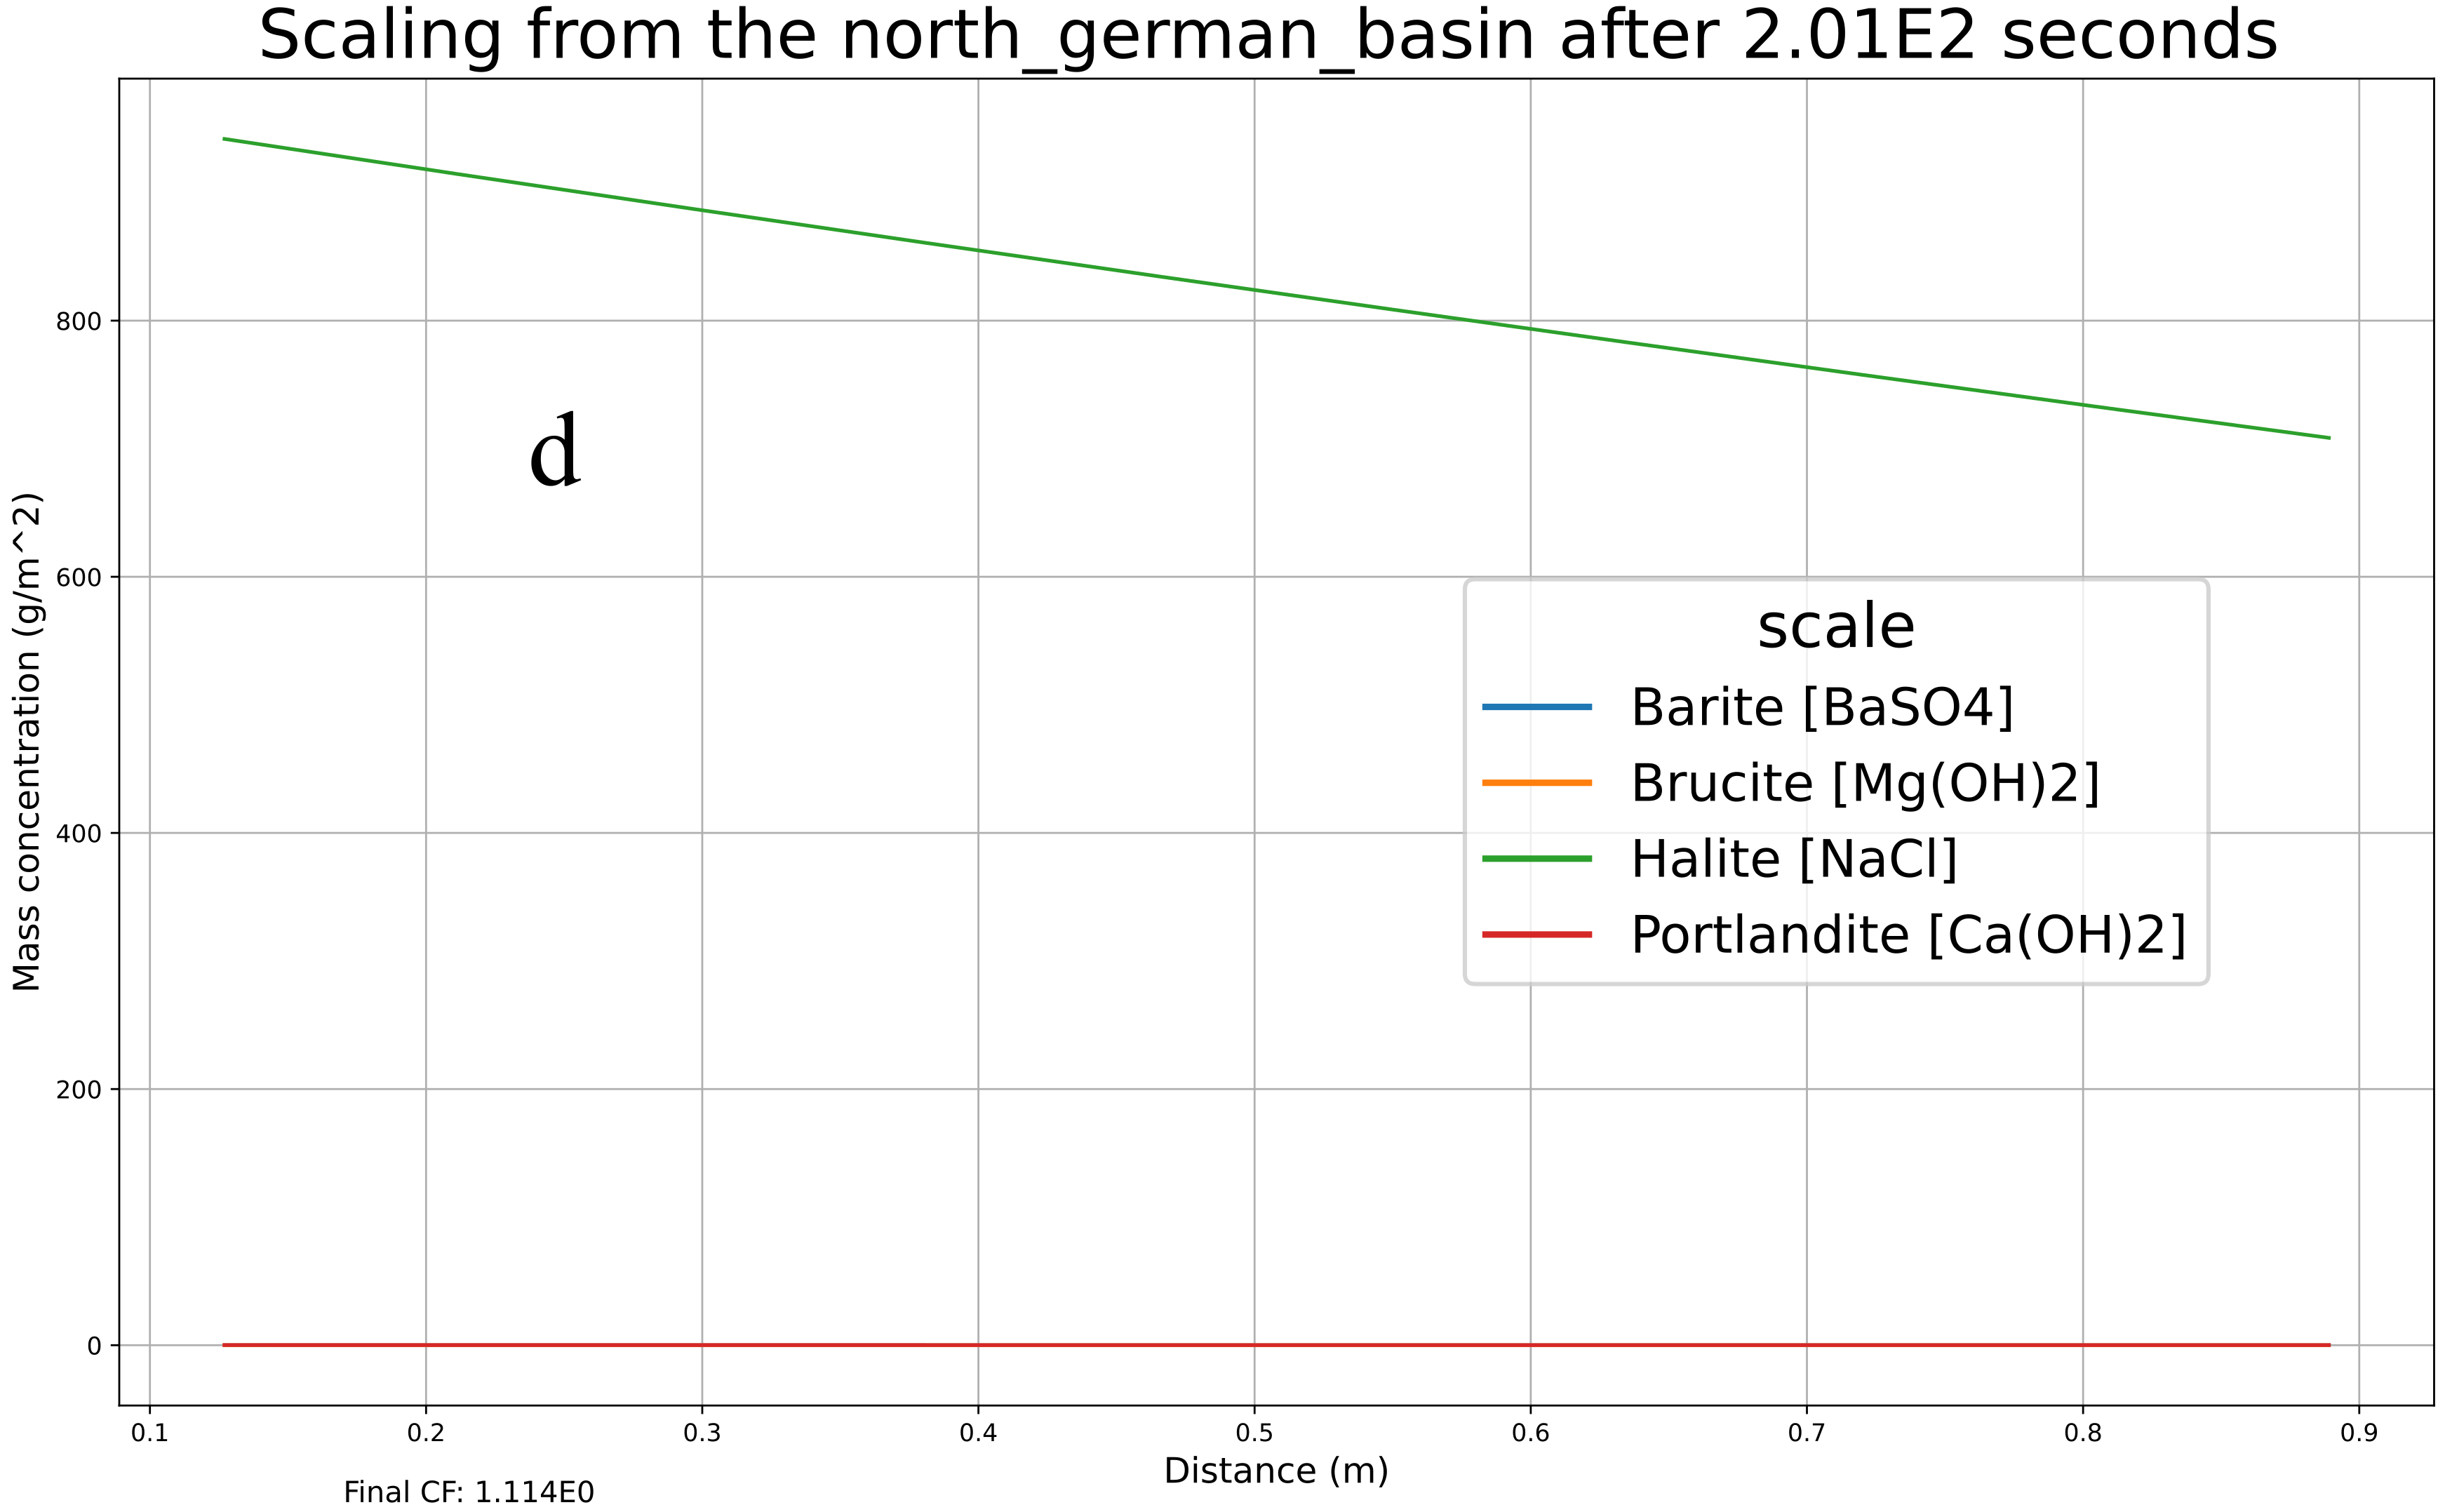
\includegraphics[width=0.49\textwidth]{images/ROSSpy/sensitivity_analyses/feed_source/German_Basin.png} \\ \bottomrule
    \end{tabular}
    \caption{
        Scaling predictions of a) the Mediterranean Sea, b) produced waters from the Palo Duro oil basin, c) the Red Sea, d) produced waters from the North German oil basin, with otherwise identical simulation parameters. These subfigures represent the spectrum of scaling predictions from the variety of different feed sources, which exhibits a high sensitivity of scale predictions to the feed geochemistry. 
    }
    \label{feed_sources}
\end{figure}

\section{Software}
ROSSpy, which is conceptualized by Figure \ref{workflow}, combines our one-dimensional RO model with post-processing operations that facilitate interpretation of the simulation results. The software a) translates parameters into a PHREEQ input file; b) executes that input file via PHREEQpy; c) processes the simulation results into figures and data tables via Matplotlib \cite{Hunter2007Matplotlib:Environment} and Pandas \cite{McKinney2011Pandas:Statistics} Python packages, respectively; and d) exports all of the simulation content -- e.g. the PHREEQ input file, SVG data figures, and CSV files of parameters, variables, data, and brine predictions -- into a specified folder and directory. The simulation data may be sliced into one-dimensional sets of distance or time that can be plotted against either scaling density or brine concentrations (Figures S2-S3) (see ROSSpy documentation).


\begin{figure}
    \centering
    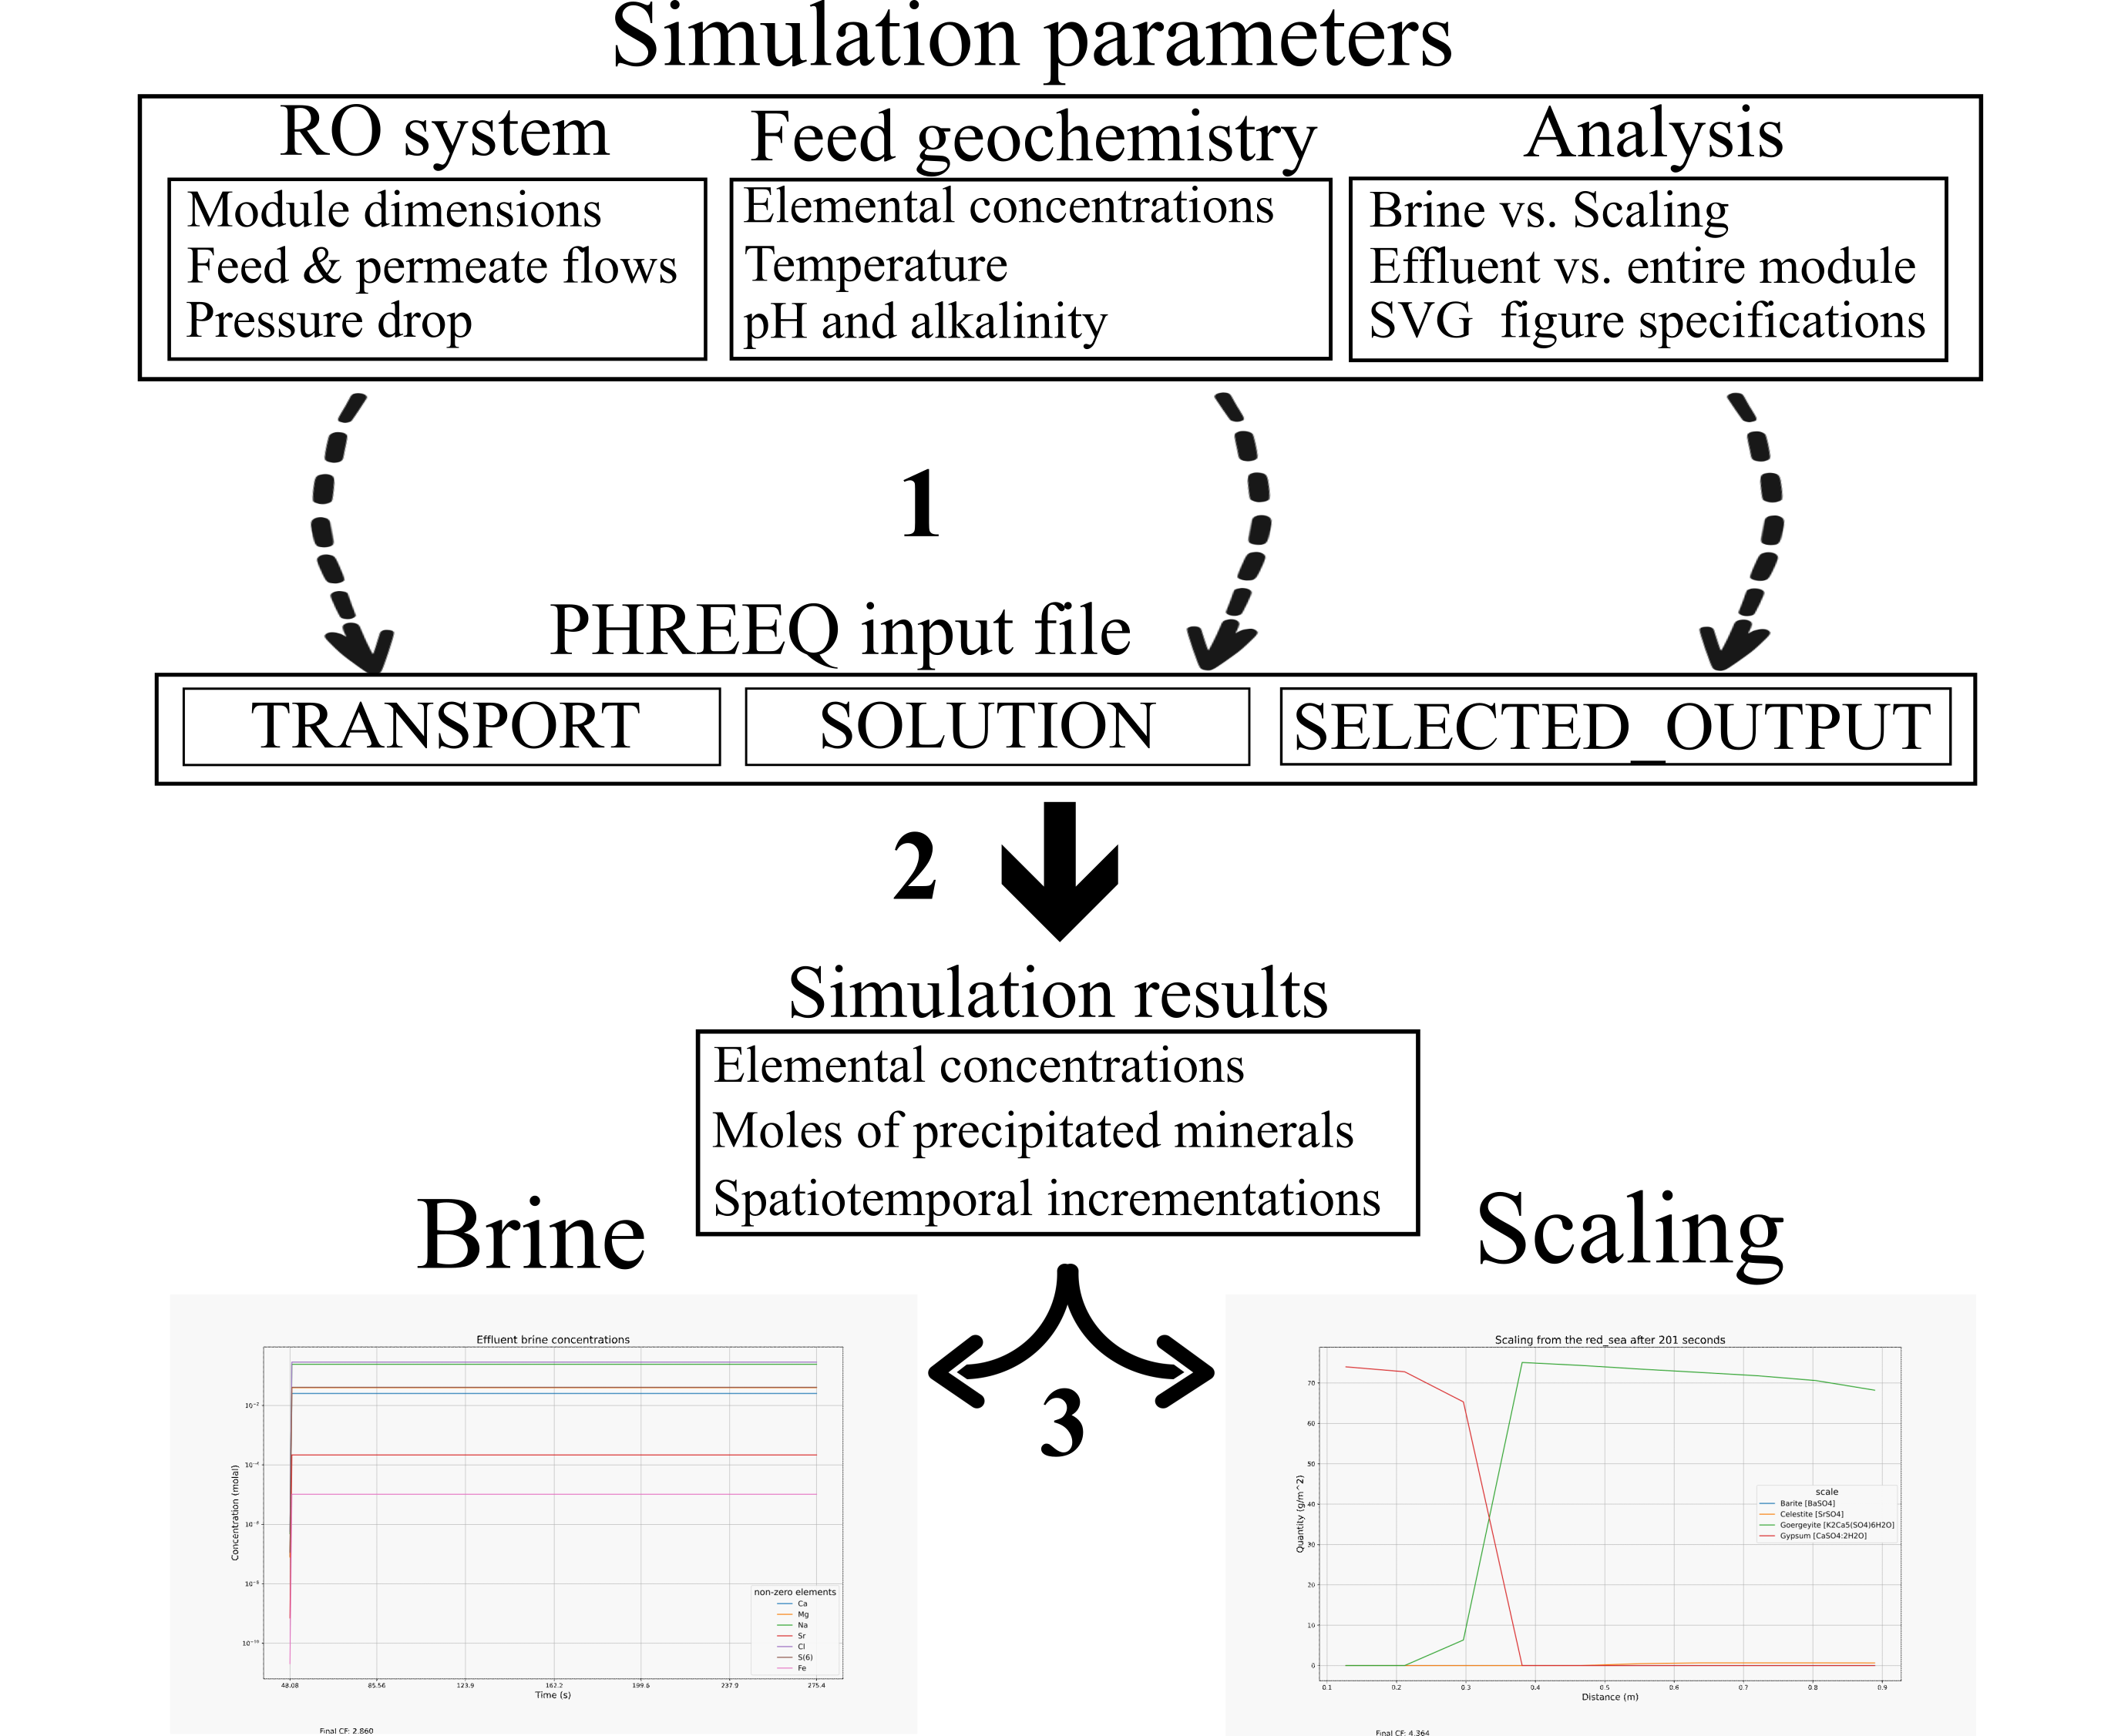
\includegraphics[width = \linewidth]{images/ROSSpy/rosspy_workflow_1.PNG}
    \caption{
        The ROSSpy workflow. Step 1 describes the translation of parameters -- i.e. module specifications, feed geochemistry, and simulation analysis -- into the corresponding code blocks of a PHREEQ input file. Step 2 describes executing the PHREEQ input file via either PHREEQpy in ROSSpy, or via the PHREEQC batch software in the interactive version of ROSSpy (iROSSpy) that is under development. Step 3 describes processing the predictions of brine concentrations or scaling quantities into representative figures and datatables, which are ultimately exported.
    }
    \label{workflow}
\end{figure}

\section{Conclusion}

A one-dimensional approximation of RO reactive transport geochemistry, executed in PHREEQC, is a practical and accurate representation of mineral scaling during desalination. The simulation predictions of this model were quantitatively and qualitatively verified for a few use cases, with both theoretical expectations and experimental data where it was available. The API implementation of this model (ROSSpy) furthermore meets identified needs of the community -- e.g. rapidly designing, executing, processing, and exporting simulations of RO scaling -- while maintaining accessibility through its light-weight design and its open-source code. We expect that this one-dimensional model and the unique attributes of ROSSpy  will facilitate scaling research and ultimately improve the efficiency of RO desalination towards alleviating chronic water insecurities in the world. 

\section{Funding}
This work was prepared in partial fulfillment of the requirements of the Berkeley Lab Undergraduate Research (BLUR) Program, managed by Workforce Development \& Education at the Berkeley Lab. The project was also partly funded by NSERC Discovery, MITACS Accelerate, CEWIL, and Canada Summer Jobs. 

% Acknowledgements section
\section{Acknowledgement}
The authors thank Ethan Sean Chan for his technical assistance in developing a graphical interface of ROSSpy (iROSSpy) that will be released in a future version. 

\appendix
\startappendix{Additional Information}
\label{chapter:appendix}

This is a good place to put tables, lots of results, perhaps all the data compiled in the experiments. By avoiding putting all the results inside the chapters themselves, the whole thing may become much more readable and the various tables can be linked to appropriately.

The main purpose of an Appendix however should be to take care of the future readers and researchers. This implies listing all the housekeeping facts needed to continue the research. For example: where is the raw data stored? where is the software used? which version of which operating system or library or experimental equipment was used and where can it be accessed again?

Ask yourself: if you were given this thesis to read with the goal that you will be expanding the research presented here, what would you like to have as housekeeping information and what do you need? Be kind to the future graduate students and to your supervisor who will be the one stuck in the middle trying to find where all the stuff was left!



% The style of bibliography exemplified here is the "plain",
% normally used in science theses. This is shown
% by the entry {plain} below. Substitute the
% appropriate bibliography style. See also the
% PDF file "InformationOnBibliographyStyles" in this
% directory for more choices.

% The Bibliography file is a BibTex file named
% UVicThesis.bib and called below

	\TOCadd{Bibliography}
	\bibliographystyle{plain}
	\bibliography{UvicThesis}

\end{document}
